\documentclass{article}

  % packages
    % basic stuff for rendering math
    \usepackage[letterpaper, top=1in, bottom=1in, left=1in, right=1in]{geometry}
    \usepackage[utf8]{inputenc}
    \usepackage[english]{babel}
    \usepackage{amsmath} 
    \usepackage{amssymb}

    % extra math symbols and utilities
    \usepackage{mathtools}        % for extra stuff like \coloneqq
    \usepackage{mathrsfs}         % for extra stuff like \mathsrc{}
    \usepackage{centernot}        % for the centernot arrow 
    \usepackage{bm}               % for better boldsymbol/mathbf 
    \usepackage{enumitem}         % better control over enumerate, itemize
    \usepackage{hyperref}         % for hypertext linking
    \usepackage{xr-hyper}
    \usepackage{fancyvrb}          % for better verbatim environments
    \usepackage{newverbs}         % for texttt{}
    \usepackage{xcolor}           % for colored text 
    \usepackage{listings}
    \usepackage{lstautogobble}
    \usepackage{parcolumns}

    \usepackage[T1]{fontenc}

    % page layout
    \usepackage{fancyhdr}         % for headers and footers 
    \usepackage{lastpage}         % to include last page number in footer 
    \usepackage{parskip}          % for no indentation and space between paragraphs    


    % for custom environments
    \usepackage{tcolorbox}        % for better colored boxes in custom environments
    \tcbuselibrary{breakable}     % to allow tcolorboxes to break across pages

    % figures
    \usepackage{pgfplots}
    \pgfplotsset{compat=1.18}
    \usepackage{float}            % for [H] figure placement
    \usepackage{tikz}
    \usepackage{tikz-cd}
    \usepackage{circuitikz}
    \usetikzlibrary{shapes.geometric}
    \usetikzlibrary{circuits.logic.US}
    \tikzset{every logic gate/.style={logic gate US}}
    \usetikzlibrary{arrows}
    \usetikzlibrary{positioning}
    \usetikzlibrary{calc}
    \usepackage{graphicx}
    \usepackage{caption} 
    \usepackage{subcaption}
    \captionsetup{font=small}

    % for tabular stuff 
    \usepackage{dcolumn}
    \usepackage{multirow}

    \usepackage[nottoc]{tocbibind}
    \pdfsuppresswarningpagegroup=1
    \hfuzz=5.002pt                % ignore overfull hbox badness warnings below this limit

  % New and replaced operators
    \DeclareMathOperator{\NOT}{NOT}
    \DeclareMathOperator{\AND}{AND}
    \DeclareMathOperator{\OR}{OR}
    \DeclareMathOperator{\NOR}{NOR}
    \DeclareMathOperator{\NAND}{NAND}
    \DeclareMathOperator{\XOR}{XOR}
    \DeclareMathOperator{\MUX}{MUX}
    \DeclareMathOperator{\DEMUX}{DEMUX}
    \newcommand{\qed}{\hfill$\blacksquare$}     % I like QED squares to be black

  % Custom Environments
    \newtcolorbox[auto counter, number within=section]{exercise}[1][]
    {
      colframe = teal!25,
      colback  = teal!10,
      coltitle = teal!20!black,  
      breakable, 
      title = \textbf{Exercise \thetcbcounter ~(#1)}
    }
    \newtcolorbox[auto counter, number within=section]{solution}[1][]
    {
      colframe = violet!25,
      colback  = violet!10,
      coltitle = violet!20!black,  
      breakable, 
      title = \textbf{Solution \thetcbcounter}
    }
    \newtcolorbox[auto counter, number within=section]{lemma}[1][]
    {
      colframe = red!25,
      colback  = red!10,
      coltitle = red!20!black,  
      breakable, 
      title = \textbf{Lemma \thetcbcounter ~(#1)}
    }
    \newtcolorbox[auto counter, number within=section]{theorem}[1][]
    {
      colframe = red!25,
      colback  = red!10,
      coltitle = red!20!black,  
      breakable, 
      title = \textbf{Theorem \thetcbcounter ~(#1)}
    } 
    \newtcolorbox[auto counter, number within=section]{corollary}[1][]
    {
      colframe = red!25,
      colback  = red!10,
      coltitle = red!20!black,  
      breakable, 
      title = \textbf{Corollary \thetcbcounter ~(#1)}
    } 
    \newtcolorbox[auto counter, number within=section]{proof}[1][]
    {
      colframe = orange!25,
      colback  = orange!10,
      coltitle = orange!20!black,  
      breakable, 
      title = \textbf{Proof. }
    } 
    \newtcolorbox[auto counter, number within=section]{definition}[1][]
    {
      colframe = yellow!25,
      colback  = yellow!10,
      coltitle = yellow!20!black,  
      breakable, 
      title = \textbf{Definition \thetcbcounter ~(#1)}
    } 
    \newtcolorbox[auto counter, number within=section]{example}[1][]
    {
      colframe = blue!25,
      colback  = blue!10,
      coltitle = blue!20!black,  
      breakable, 
      title = \textbf{Example \thetcbcounter ~(#1)}
    } 
    \newtcolorbox[auto counter, number within=section]{imp}[1][]
    {
      colframe = green!25,
      colback  = green!10,
      coltitle = green!20!black,  
      breakable, 
      title = \textbf{Implementation \thetcbcounter ~(#1)}
    } 
    \definecolor{dkgreen}{rgb}{0,0.6,0}
    \definecolor{gray}{rgb}{0.5,0.5,0.5}
    \definecolor{mauve}{rgb}{0.58,0,0.82}
    \definecolor{lightgray}{gray}{0.93}
    \lstset{
      autogobble,
      frame=ltbr,
      language=Verilog,
      aboveskip=3mm,
      belowskip=3mm,
      showstringspaces=false,
      columns=fullflexible,
      keepspaces=true,
      basicstyle={\small\ttfamily},
      numbers=left,
      firstnumber=1, 
      numberstyle=\tiny\color{gray},
      keywordstyle=\color{blue},
      commentstyle=\color{dkgreen},
      stringstyle=\color{mauve},
      backgroundcolor=\color{lightgray}, 
      breaklines=true,
      breakatwhitespace=true,
      tabsize=3, 
      xleftmargin=2em, 
      framexleftmargin=1.5em, 
      stepnumber=1
    }

  % Page style
    \pagestyle{fancy}
    \fancyhead[L]{Computer Architecture}
    \fancyhead[C]{Muchang Bahng}
    \fancyhead[R]{Spring 2024} 
    \fancyfoot[C]{\thepage / \pageref{LastPage}}
    \renewcommand{\footrulewidth}{0.4pt}          % the footer line should be 0.4pt wide
    \renewcommand{\thispagestyle}[1]{}  % needed to include headers in title page

    \externaldocument[th-]{../Theory/paper}[../Theory/paper.pdf] 
    \externaldocument[dsa-]{../DSA/paper}[../DSA/paper.pdf] 
    \externaldocument[set-]{../../Math/Set_Theory/paper}[../../Math/Set_Theory/paper.pdf]

\begin{document}

\title{Computer Architecture}
\author{Muchang Bahng}
\date{Spring 2024}

\maketitle
\tableofcontents
\pagebreak

This covers computability theory, complexity theory, and automata theory. 
Alphabet. Boolean logic


\section{Transistors}

  Note that \textit{computation} is an abstract notion (a process) that is distinct from its physical \textit{implementations} (how the progress is run). While most modern computing devices are obtained by mapping logical gates to semiconductor-based transistors, throughout history people have computed using a huge variety of mechanisms, including mechanical systems, gas and liquid (known as fluidics), biological and chemical processes, and even living creatures. 

  \begin{example}[Biological Computing]
    Computation can be based on biological or chemical systems. For example the lac-operon produces the enzymes needed to digest lactose only if the conditions $x \wedge (\lnot y)$ hold, where $x$ is ``lactose is present'' and $y$ is ``glucose is present.''
  \end{example}

  \begin{example}[Cellular Automata and the Game of Life]
    Cellular automata is a model of a system composed of a sequence of cells, each of which can have a finite state. At each step, a cell updates its state based on the states of its neighboring cells and some simple rules. As we will discuss later in this book, cellular automata such as Conway’s \textit{Game of Life} can be used to simulate computation gates.
  \end{example}

  \begin{example}[Neural Network]
    Another computation device is the brain. Even though the exact working of the brain is still not fully understood, one common mathematical model for it is a (very large) \textbf{neural network}. A neural network can be thought of as a circuit that---instead of AND/OR/NOT---uses other gates as the basic basis. One particular basis we can use are \textbf{threshold gates}, which exist through action potentials n neurons. Approximations of this simulation have been made through artificial netural networks: For every vector $w \in \mathbb{R}^k, t \in \mathbb{Z}$, the threshold function corresponding to $w, t$ is the function 
    \begin{equation}
      T_{w, t} :\{0,1\}^k \longrightarrow \{0,1\}, \qquad T_{w, t}(x) = 1 \text{ iff } \langle w, x \rangle \geq t
    \end{equation}
    where $\langle \cdot, \cdot \rangle$ represents the dot product. To a first approximation, a neuron has $k$ inputs and a single output, and the neurons “fires” or “turns on” its output when those signals pass some threshold. 
  \end{example}

  A transistor can be thought of as an electric circuit with two inputs, known as the source and the gate and an output, known as the sink. The gate controls whether current flows from the source to the sink. In a standard transistor, if the gate is “ON” then current can flow from the source to the sink and if it is “OFF” then it can’t. In a complementary transistor this is reversed: if the gate is “OFF” then current can flow from the source to the sink and if it is “ON” then it can’t. 

  We can use transistors to implement various Boolean functions such as and AND, OR, and NOT. For each a two-input gate $G: \{0,1\}^2 \longrightarrow \{0,1\}$, such an implementation would be a system with two input wires $x, y$ and one output wire $z$, such that if we identify high---as in passes a \textbf{threshold voltage}---voltage with $1$ and low voltage with $0$, then the wire $z$ will equal to $1$ if and only if applying $G$ to the values of the wires $x$ and $y$ is $1$. 

\subsection{Semiconductors}

  Okay, basic electronic construction and physics. Some substances are able to easily gain or lose electrons. These allow electricity to flow well, as electrical current is simply electrons moving around. These are "conductors." Other substances are highly resistant to gaining or losing electrons, which means they do not allow electricity to flow well. These are called "insulators."

  There is a third kind of substance that falls in between them, that holds on to its electrons harder than conductors but not as hard as insulators. They are called "semiconductors," of which silicon is the most important one. 

  Since everything that happens here is on the atomic level, it is very easy to make transistors on the small scale. A mechanical switch with copper contacts would have to be much larger than a transistor. Copper is a conductor, one of the best ones we have, so electrons can jump from one contact to another over a "decent distance." A gap of a couple millimeters is enough to break the circuit, but compared to transistors, that's a massive gulf. Plus, you need something to mechanically move the contacts. Usually an electromagnet is used. Put an electromagnet in a formation that it will cause contacts to open or close when the magnet is energized, and you have a "relay." That's what we used before transistors, and are often used today, though we no longer use them for "thinking" in electronics.

  But with semiconductors, they can change from being a conductor to being an insulator very easily. The trick is to add just the right amount of impurities in just the right structure. This is called "doping," and in the world of electronics, it's a good thing. All it takes is a single atom to switch a properly doped piece of silicon from an insulator to conductor and back again. Plus the process is purely electronic. There are no moving parts, so no mechanical components are needed. All you need to do is apply an electrical current to the third leg of a transistor, and the other two legs will go from "open" to "closed." Once the current on the third leg stops, the transistor "opens" again and electricity can't pass through. 

  You want semiconductors since. 

  You first make silicon wafers. 

\subsection{Doping}



\section{Sequential Chips}

  Now that we know how the NAND gate---and therefore every other fundamental gate---works, and we have constructed the clock, the next natural step is to be able to store a string of bits.\footnote{Most courses teach combinational logic first and then sequential, but this may not be the most optimal dependency sequence for two reasons. We can indeed do arithmetic without memory by directly applying an electric current to the input wires in a circuit, but this severely limits the computation that we can do. We would essentially have to do everything in ``one shot'' and immediately collect the results. While this is fine for addition, I cannot introduce an efficient schema of multiplication without knowing how to bit-shift, which is dependent on some form of memory. On a broader scale, almost all algorithms we worked with require some memory at some point, so memory may be more fundamental than computation. Thanks the Phillip Williams for talking with me on this!} Computers must be equipped with memory elements that can preserve data over time. These memory elements are built from \textit{sequential chips}. 

\subsection{Latches}

  Ideally, we would like a way to store a bit in memory, and this can be done by cross-coupling gates with each other, forming a sort of positive feedback.\footnote{Note that unlike combinational logic, this now deviates from straight-line programming.} Therefore, given a certain signal into our circuit which we call a \textit{latch}, the outputs remain locked---or ``latched''---into a state. 

  \begin{definition}[SR Latch]
    The \textbf{set-reset (SR) latch} is a circuit that stores 1-bit memory. This is based on \textit{pulses} and we do not care about the duration of a signal. That is, if we activate a signal to inputs $S, R$ at \textit{any} point in time, then the output $Q$ will remain locked in some state, even \textit{after} the input signal disappears. 
  \end{definition}

  The SR latch---like all electronic circuits---require power to work, labeled with $S$ and $R$. The output is really just $Q$, but we can add redundancy by making the inverse $\overline{Q}$ available as well. There are two implementations of an SRlatch, which have symmetric behaviors. 

  \begin{theorem}[Active High SR Latch]
    A NOR SR latch can be implemented in the following circuit below, with its corresponding truth table. 

    \begin{figure}[H]
      \centering
      \begin{subfigure}[b]{0.48\textwidth}
        \centering
        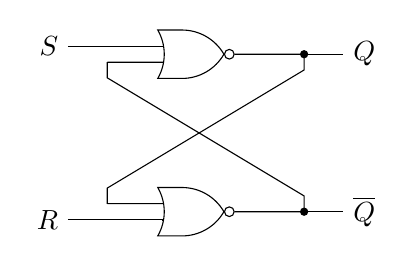
\begin{tikzpicture}[circuit logic US]
          \node[nor gate] (nor1) at (0, 1) {}; 
          \node[nor gate] (nor2) at (0, -1) {}; 

          \node[left] at (-1.5, 1.1) {$S$}; 
          \node[left] at (-1.5, -1.1) {$R$}; 
          \node[right] at (2, 1) {$Q$};
          \node[right] at (2, -1) {$\overline{Q}$};

          \draw (-1.5, 1.1) -| (nor1.input 1);
          \draw (-1.5, -1.1) -| (nor2.input 2);
          \draw (nor1.output) |- (2, 1); 
          \draw (nor2.output) |- (2, -1); 

          \draw (nor1.output) |- (1.5, 1) -- (1.5, 0.8) -- (-1, -0.7) -- (-1, -0.9) |- (nor2.input 1);
          \draw (nor2.output) |- (1.5, -1) -- (1.5, -0.8) -- (-1, 0.7) -- (-1, 0.9) |- (nor1.input 2);
          \fill (1.5,1) circle (1.5pt);
          \fill (1.5,-1) circle (1.5pt);
        \end{tikzpicture} 
        \caption{Circuit diagram.}
      \end{subfigure}
      \hfill 
      \begin{subfigure}[b]{0.48\textwidth}
        \centering
        \begin{tabular}{|c|c|c|c|}
          \hline
          \textbf{S} & \textbf{R} & \textbf{Q} & \textbf{$\overline{Q}$} \\
          \hline
          0 & 0 & 1 & 0 \\
            &   & 0 & 1 \\
          \hline
          0 & 1 & 0 & 1 \\
          \hline
          1 & 0 & 1 & 0 \\
          \hline
          1 & 1 & 0 & 0 \\
          \hline
        \end{tabular} 
        \caption{Truth table.}
      \end{subfigure}
      \caption{XOR SR Latch. This is }
    \end{figure}

    Setting both $R = S = 1$ would result in an invalid state since they would attempt to turn $Q$ back and forth between $0$ and $1$, giving us a race condition. 

    \begin{figure}[H]
      \centering
      \begin{subfigure}[b]{0.48\textwidth}
        \centering
        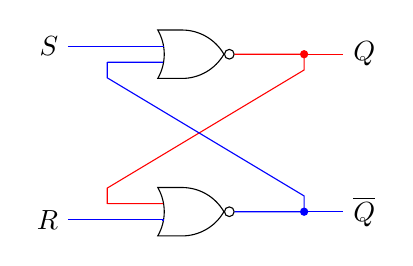
\begin{tikzpicture}[circuit logic US]
          \node[nor gate] (nor1) at (0, 1) {}; 
          \node[nor gate] (nor2) at (0, -1) {}; 

          \node[left] at (-1.5, 1.1) {$S$}; 
          \node[left] at (-1.5, -1.1) {$R$}; 
          \node[right] at (2, 1) {$Q$};
          \node[right] at (2, -1) {$\overline{Q}$};

          \draw[blue] (-1.5, 1.1) -| (nor1.input 1);
          \draw[blue] (-1.5, -1.1) -| (nor2.input 2);
          \draw[red] (nor1.output) |- (2, 1); 
          \draw[blue] (nor2.output) |- (2, -1); 

          \draw[red] (nor1.output) |- (1.5, 1) -- (1.5, 0.8) -- (-1, -0.7) -- (-1, -0.9) |- (nor2.input 1);
          \draw[blue] (nor2.output) |- (1.5, -1) -- (1.5, -0.8) -- (-1, 0.7) -- (-1, 0.9) |- (nor1.input 2);
          \fill[red] (1.5,1) circle (1.5pt);
          \fill[blue] (1.5,-1) circle (1.5pt);
        \end{tikzpicture} 
        \caption{}
      \end{subfigure}
      \hfill 
      \begin{subfigure}[b]{0.48\textwidth}
        \centering
        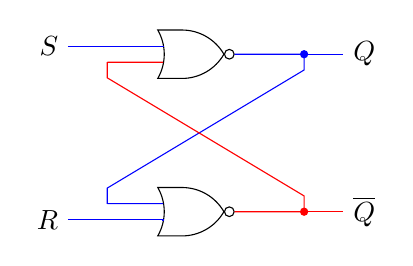
\begin{tikzpicture}[circuit logic US]
          \node[nor gate] (nor1) at (0, 1) {}; 
          \node[nor gate] (nor2) at (0, -1) {}; 

          \node[left] at (-1.5, 1.1) {$S$}; 
          \node[left] at (-1.5, -1.1) {$R$}; 
          \node[right] at (2, 1) {$Q$};
          \node[right] at (2, -1) {$\overline{Q}$};

          \draw[blue] (-1.5, 1.1) -| (nor1.input 1);
          \draw[blue] (-1.5, -1.1) -| (nor2.input 2);
          \draw[blue] (nor1.output) |- (2, 1); 
          \draw[red] (nor2.output) |- (2, -1); 

          \draw[blue] (nor1.output) |- (1.5, 1) -- (1.5, 0.8) -- (-1, -0.7) -- (-1, -0.9) |- (nor2.input 1);
          \draw[red] (nor2.output) |- (1.5, -1) -- (1.5, -0.8) -- (-1, 0.7) -- (-1, 0.9) |- (nor1.input 2);
          \fill[blue] (1.5,1) circle (1.5pt);
          \fill[red] (1.5,-1) circle (1.5pt);
        \end{tikzpicture} 
        \caption{}
      \end{subfigure}
      \caption{Two possible initial states. The default state is $R = 0, S = 0$, which are both \textit{low states}, and $Q$ may be either $0$ or $1$. }
    \end{figure}

    If one of $R$ or $S$ is set to a high state, the latch is activated, and hence this is called an \textbf{active high SR latch}. Note that regardless of what the previous state the latch was in, the output signals are completely determined. 

    \begin{figure}[H]
      \centering
      \begin{subfigure}[b]{0.48\textwidth}
        \centering
        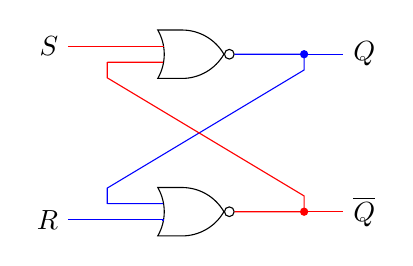
\begin{tikzpicture}[circuit logic US]
          \node[nor gate] (nor1) at (0, 1) {}; 
          \node[nor gate] (nor2) at (0, -1) {}; 

          \node[left] at (-1.5, 1.1) {$S$}; 
          \node[left] at (-1.5, -1.1) {$R$}; 
          \node[right] at (2, 1) {$Q$};
          \node[right] at (2, -1) {$\overline{Q}$};

          \draw[red] (-1.5, 1.1) -| (nor1.input 1);
          \draw[blue] (-1.5, -1.1) -| (nor2.input 2);
          \draw[blue] (nor1.output) |- (2, 1); 
          \draw[red] (nor2.output) |- (2, -1); 

          \draw[blue] (nor1.output) |- (1.5, 1) -- (1.5, 0.8) -- (-1, -0.7) -- (-1, -0.9) |- (nor2.input 1);
          \draw[red] (nor2.output) |- (1.5, -1) -- (1.5, -0.8) -- (-1, 0.7) -- (-1, 0.9) |- (nor1.input 2);
          \fill[blue] (1.5,1) circle (1.5pt);
          \fill[red] (1.5,-1) circle (1.5pt);
        \end{tikzpicture} 
        \caption{If we send a signal $R = 1$, then $Q = 0$, and even if we reset $R = 0$, $Q$ is still locked at $0$. }
      \end{subfigure}
      \hfill 
      \begin{subfigure}[b]{0.48\textwidth}
        \centering
        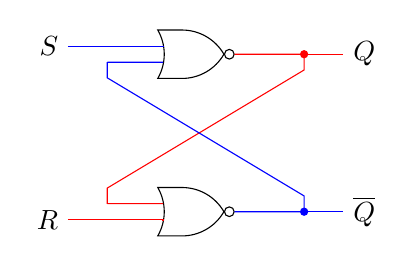
\begin{tikzpicture}[circuit logic US]
          \node[nor gate] (nor1) at (0, 1) {}; 
          \node[nor gate] (nor2) at (0, -1) {}; 

          \node[left] at (-1.5, 1.1) {$S$}; 
          \node[left] at (-1.5, -1.1) {$R$}; 
          \node[right] at (2, 1) {$Q$};
          \node[right] at (2, -1) {$\overline{Q}$};

          \draw[blue] (-1.5, 1.1) -| (nor1.input 1);
          \draw[red] (-1.5, -1.1) -| (nor2.input 2);
          \draw[red] (nor1.output) |- (2, 1); 
          \draw[blue] (nor2.output) |- (2, -1); 

          \draw[red] (nor1.output) |- (1.5, 1) -- (1.5, 0.8) -- (-1, -0.7) -- (-1, -0.9) |- (nor2.input 1);
          \draw[blue] (nor2.output) |- (1.5, -1) -- (1.5, -0.8) -- (-1, 0.7) -- (-1, 0.9) |- (nor1.input 2);
          \fill[red] (1.5,1) circle (1.5pt);
          \fill[blue] (1.5,-1) circle (1.5pt);
        \end{tikzpicture} 
        \caption{If we send a signal $S = 1$, then $Q = 1$, and even if reset $S = 0$, $Q$ is still locked at $1$. }
      \end{subfigure}
      \caption{}
    \end{figure}
  \end{theorem}

  Now unlike the active high latches which are activated when the current is $1$, active low latches are activated when the current is $0$. 

  \begin{theorem}[Active Low SR Latch]
    A NAND SR latch can be implemented in the following circuit below, with its corresponding truth table. 
    
    \begin{figure}[H]
      \centering
      \begin{subfigure}[b]{0.48\textwidth}
        \centering
        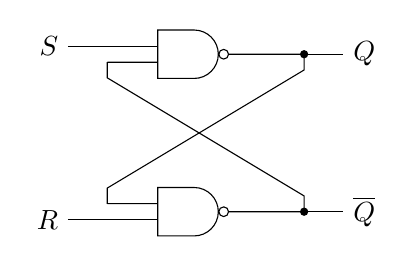
\begin{tikzpicture}[circuit logic US]
          \node[nand gate] (nor1) at (0, 1) {}; 
          \node[nand gate] (nor2) at (0, -1) {}; 
          \node[left] at (-1.5, 1.1) {$S$}; 
          \node[left] at (-1.5, -1.1) {$R$}; 
          \node[right] at (2, 1) {$Q$};
          \node[right] at (2, -1) {$\overline{Q}$};

          \draw (-1.5, 1.1) -| (nor1.input 1);
          \draw (-1.5, -1.1) -| (nor2.input 2);
          \draw (nor1.output) |- (2, 1); 
          \draw (nor2.output) |- (2, -1); 

          \draw (nor1.output) |- (1.5, 1) -- (1.5, 0.8) -- (-1, -0.7) -- (-1, -0.9) |- (nor2.input 1);
          \draw (nor2.output) |- (1.5, -1) -- (1.5, -0.8) -- (-1, 0.7) -- (-1, 0.9) |- (nor1.input 2);
          \fill (1.5,1) circle (1.5pt);
          \fill (1.5,-1) circle (1.5pt);
        \end{tikzpicture} 
        \caption{Circuit diagram.}
      \end{subfigure}
      \hfill 
      \begin{subfigure}[b]{0.48\textwidth}
        \centering
        \begin{tabular}{|c|c|c|c|}
          \hline
          \textbf{S} & \textbf{R} & \textbf{Q} & \textbf{$\overline{Q}$} \\
          \hline
          0 & 0 & 1 & 1 \\
          \hline
          0 & 1 & 1 & 0 \\
          \hline
          1 & 0 & 0 & 1 \\
          \hline
          1 & 1 & 0 & 1 \\
            &   & 1 & 0 \\
          \hline
        \end{tabular}
        \caption{Truth table.}
      \end{subfigure}
      \caption{NAND SR Latch}
    \end{figure}

    Setting both $R = S = 0$ would result in an invalid state since they would attempt to turn $Q$ back and forth between $0$ and $1$, giving us a race condition. 

    \begin{figure}[H]
      \centering
      \begin{subfigure}[b]{0.48\textwidth}
        \centering
        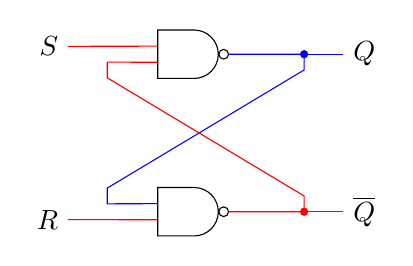
\begin{tikzpicture}[circuit logic US]
          \node[nand gate] (nor1) at (0, 1) {}; 
          \node[nand gate] (nor2) at (0, -1) {}; 
          \node[left] at (-1.5, 1.1) {$S$}; 
          \node[left] at (-1.5, -1.1) {$R$}; 
          \node[right] at (2, 1) {$Q$};
          \node[right] at (2, -1) {$\overline{Q}$};

          \draw[red] (-1.5, 1.1) -- (nor1.input 1);
          \draw[red] (-1.5, -1.1) -- (nor2.input 2);
          \draw[blue] (nor1.output) -- (2, 1); 
          \draw[red] (nor2.output) -- (2, -1); 

          \draw[blue] (nor1.output) -- (1.5, 1) -- (1.5, 0.8) -- (-1, -0.7) -- (-1, -0.9) -- (nor2.input 1);
          \draw[red] (nor2.output) -- (1.5, -1) -- (1.5, -0.8) -- (-1, 0.7) -- (-1, 0.9) -- (nor1.input 2);
          \fill[blue] (1.5,1) circle (1.5pt);
          \fill[red] (1.5,-1) circle (1.5pt);
        \end{tikzpicture} 
        \caption{}
      \end{subfigure}
      \hfill 
      \begin{subfigure}[b]{0.48\textwidth}
        \centering
        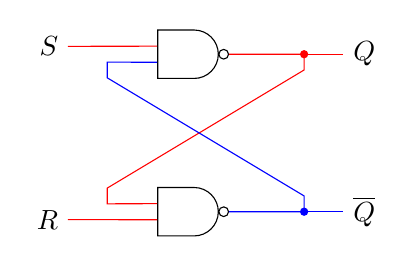
\begin{tikzpicture}[circuit logic US]
          \node[nand gate] (nor1) at (0, 1) {}; 
          \node[nand gate] (nor2) at (0, -1) {}; 
          \node[left] at (-1.5, 1.1) {$S$}; 
          \node[left] at (-1.5, -1.1) {$R$}; 
          \node[right] at (2, 1) {$Q$};
          \node[right] at (2, -1) {$\overline{Q}$};

          \draw[red] (-1.5, 1.1) -- (nor1.input 1);
          \draw[red] (-1.5, -1.1) -- (nor2.input 2);
          \draw[red] (nor1.output) -- (2, 1); 
          \draw[blue] (nor2.output) -- (2, -1); 

          \draw[red] (nor1.output) -- (1.5, 1) -- (1.5, 0.8) -- (-1, -0.7) -- (-1, -0.9) -- (nor2.input 1);
          \draw[blue] (nor2.output) -- (1.5, -1) -- (1.5, -0.8) -- (-1, 0.7) -- (-1, 0.9) -- (nor1.input 2);
          \fill[red] (1.5,1) circle (1.5pt);
          \fill[blue] (1.5,-1) circle (1.5pt);
        \end{tikzpicture} 
        \caption{}
      \end{subfigure}
      \caption{The default state is $R = 1, S = 1$, i.e. they are both \textit{high states}, and $Q$ may be either $0$ or $1$. This is known as an \textbf{active low SR latch}. }
    \end{figure}

    If one of $R$ or $S$ is set to a low state, the latch is activated, and hence this is called an \textbf{active low SR latch}. Note that regardless of what the previous state the latch was in, the output signals are completely determined. 

    \begin{figure}[H]
      \centering
      \begin{subfigure}[b]{0.48\textwidth}
        \centering
        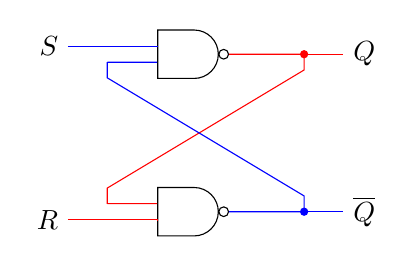
\begin{tikzpicture}[circuit logic US]
          \node[nand gate] (nor1) at (0, 1) {}; 
          \node[nand gate] (nor2) at (0, -1) {}; 
          \node[left] at (-1.5, 1.1) {$S$}; 
          \node[left] at (-1.5, -1.1) {$R$}; 
          \node[right] at (2, 1) {$Q$};
          \node[right] at (2, -1) {$\overline{Q}$};

          \draw[blue] (-1.5, 1.1) -| (nor1.input 1);
          \draw[red] (-1.5, -1.1) -| (nor2.input 2);
          \draw[red] (nor1.output) |- (2, 1); 
          \draw[blue] (nor2.output) |- (2, -1); 

          \draw[red] (nor1.output) |- (1.5, 1) -- (1.5, 0.8) -- (-1, -0.7) -- (-1, -0.9) |- (nor2.input 1);
          \draw[blue] (nor2.output) |- (1.5, -1) -- (1.5, -0.8) -- (-1, 0.7) -- (-1, 0.9) |- (nor1.input 2);
          \fill[red] (1.5,1) circle (1.5pt);
          \fill[blue] (1.5,-1) circle (1.5pt);
        \end{tikzpicture} 
        \caption{}
      \end{subfigure}
      \hfill 
      \begin{subfigure}[b]{0.48\textwidth}
        \centering
        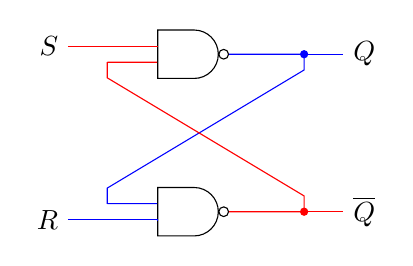
\begin{tikzpicture}[circuit logic US]
          \node[nand gate] (nor1) at (0, 1) {}; 
          \node[nand gate] (nor2) at (0, -1) {}; 
          \node[left] at (-1.5, 1.1) {$S$}; 
          \node[left] at (-1.5, -1.1) {$R$}; 
          \node[right] at (2, 1) {$Q$};
          \node[right] at (2, -1) {$\overline{Q}$};

          \draw[red] (-1.5, 1.1) -| (nor1.input 1);
          \draw[blue] (-1.5, -1.1) -| (nor2.input 2);
          \draw[blue] (nor1.output) |- (2, 1); 
          \draw[red] (nor2.output) |- (2, -1); 

          \draw[blue] (nor1.output) |- (1.5, 1) -- (1.5, 0.8) -- (-1, -0.7) -- (-1, -0.9) |- (nor2.input 1);
          \draw[red] (nor2.output) |- (1.5, -1) -- (1.5, -0.8) -- (-1, 0.7) -- (-1, 0.9) |- (nor1.input 2);
          \fill[blue] (1.5,1) circle (1.5pt);
          \fill[red] (1.5,-1) circle (1.5pt);
        \end{tikzpicture} 
        \caption{}
      \end{subfigure}
      \caption{If we send a signal $S = 0$, then $Q = 0$, and even if reset $S = 1$, $Q$ is still locked at $0$. }
    \end{figure}
  \end{theorem}

  These signals may be noisy, and we might want more control over whether a latch can change states, i.e its \textit{transparency}. This is done by adding an extra \textit{gate} that explicitly tells us when the latch can change states. 

  \begin{definition}[Gated SR Latch]
    A \textbf{gated SR latch} is an SR latch that can only change state when it is enabled. This enabling is done with an additional 2 NAND gates, and so the SR latch is enabled only when $E = 1$. 

    \begin{figure}[H]
      \centering
      \begin{subfigure}[b]{0.48\textwidth}
        \centering
        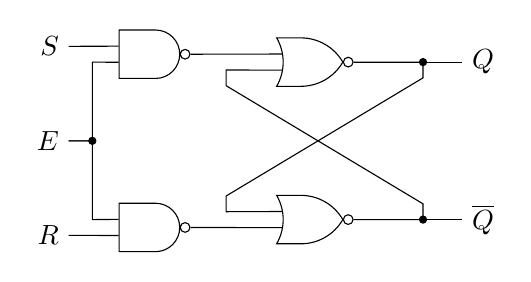
\begin{tikzpicture}[circuit logic US]
          \node[nand gate] (nand1) at (-2, 1.1) {};
          \node[nand gate] (nand2) at (-2, -1.1) {};
          \node[nor gate] (nor1) at (0, 1) {}; 
          \node[nor gate] (nor2) at (0, -1) {}; 

          \draw (-3, 1.2) -- (nand1.input 1);
          \draw (-3, -1.2) -- (nand2.input 2);
          \draw (-3, 0) -- (-2.7, 0) -- (-2.7,1) -- (nand1.input 2);
          \draw (-3, 0) -- (-2.7, 0) -- (-2.7,-1) -- (nand2.input 1);
          \node[left] at (-3,0) {$E$};
          \node[left] at (-3,1.2) {$S$};
          \node[left] at (-3,-1.2) {$R$};
          \node[right] at (2, 1) {$Q$};
          \node[right] at (2, -1) {$\overline{Q}$};

          \draw (nand1.output) -- (nor1.input 1);
          \draw (nand2.output) -- (nor2.input 2);
          \draw (nor1.output) -- (2, 1); 
          \draw (nor2.output) -- (2, -1); 

          \draw (nor1.output) -- (1.5, 1) -- (1.5, 0.8) -- (-1, -0.7) -- (-1, -0.9) -- (nor2.input 1);
          \draw (nor2.output) -- (1.5, -1) -- (1.5, -0.8) -- (-1, 0.7) -- (-1, 0.9) -- (nor1.input 2);
          \fill (1.5,1) circle (1.5pt);
          \fill (1.5,-1) circle (1.5pt);
          \fill (-2.7,0) circle (1.5pt);
        \end{tikzpicture} 
        \caption{Gated XOR SR Latch.}
      \end{subfigure}
      \hfill 
      \begin{subfigure}[b]{0.48\textwidth}
        \centering
        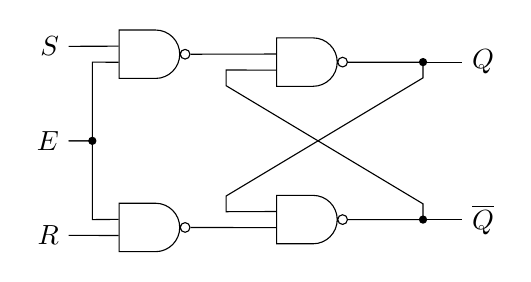
\begin{tikzpicture}[circuit logic US]
          \node[nand gate] (nand1) at (-2, 1.1) {};
          \node[nand gate] (nand2) at (-2, -1.1) {};
          \node[nand gate] (nor1) at (0, 1) {}; 
          \node[nand gate] (nor2) at (0, -1) {}; 

          \draw (-3, 1.2) -- (nand1.input 1);
          \draw (-3, -1.2) -- (nand2.input 2);
          \draw (-3, 0) -- (-2.7, 0) -- (-2.7,1) -- (nand1.input 2);
          \draw (-3, 0) -- (-2.7, 0) -- (-2.7,-1) -- (nand2.input 1);
          \node[left] at (-3,0) {$E$};
          \node[left] at (-3,1.2) {$S$};
          \node[left] at (-3,-1.2) {$R$};
          \node[right] at (2, 1) {$Q$};
          \node[right] at (2, -1) {$\overline{Q}$};

          \draw (nand1.output) -- (nor1.input 1);
          \draw (nand2.output) -- (nor2.input 2);
          \draw (nor1.output) -- (2, 1); 
          \draw (nor2.output) -- (2, -1); 

          \draw (nor1.output) -- (1.5, 1) -- (1.5, 0.8) -- (-1, -0.7) -- (-1, -0.9) -- (nor2.input 1);
          \draw (nor2.output) -- (1.5, -1) -- (1.5, -0.8) -- (-1, 0.7) -- (-1, 0.9) -- (nor1.input 2);
          \fill (1.5,1) circle (1.5pt);
          \fill (1.5,-1) circle (1.5pt);
          \fill (-2.7,0) circle (1.5pt);
        \end{tikzpicture} 
        \caption{Gated NAND SR Latch.}
      \end{subfigure}
      \caption{Note that if $E = 0$, then the output of the leftmost two NAND gates will be $1$ no matter what, and so the values of $R, S$ does not have any effect. }
    \end{figure}
  \end{definition}

  \begin{example}[Active High Gated SR Latch]
    By keeping track of the voltages in the wires of interest and running them across a common time axis, we can visualize this circuit in action. Note that in here, we assume that electric current is instantaneous, resulting in the familiar \textit{square waves}. Let's look at an active high SR latch. 

    \begin{figure}[H]
      \centering 
      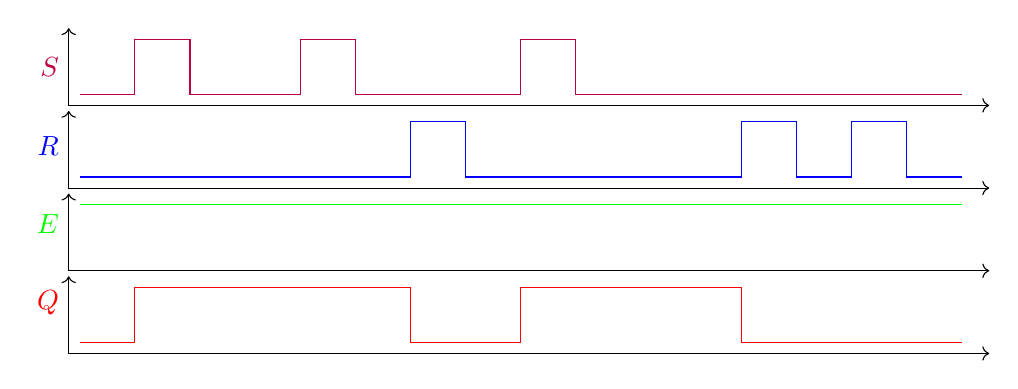
\begin{tikzpicture}[scale=0.7]
        \def\h{1.5}
        \draw[<->] (-0.2, 1.2) -- (-0.2, -0.2) -- (16.5, -0.2); 
        \draw[<->, yshift=-1.5cm] (-0.2, 1.2) -- (-0.2, -0.2) -- (16.5, -0.2); 
        \draw[<->, yshift=-3cm] (-0.2, 1.2) -- (-0.2, -0.2) -- (16.5, -0.2); 
        \draw[<->, yshift=-4.5cm] (-0.2, 1.2) -- (-0.2, -0.2) -- (16.5, -0.2); 
        \node[purple, left] at (-0.2, 0.5) {$S$}; 
        \node[blue, left, yshift=-1cm] at (-0.2, 0.5) {$R$}; 
        \node[green, left, yshift=-2cm] at (-0.2, 0.5) {$E$}; 
        \node[red, left, yshift=-3cm] at (-0.2, 0.5) {$Q$}; 

        \draw[purple] (0, 0) -- (1, 0) -- (1, 1) -- (2, 1) -- (2, 0) -- (4, 0) -- (4, 1) -- (5, 1) -- (5, 0) -- (8, 0) -- (8, 1) -- (9, 1) -- (9, 0) -- (16, 0);
        \draw[blue, yshift=-1.5cm] (0, 0) -- (6, 0) -- (6, 1) -- (7, 1) -- (7, 0) -- (12, 0) -- (12, 1) -- (13, 1) -- (13, 0) -- (14, 0) -- (14, 1) -- (15, 1) -- (15, 0) -- (16, 0);
        \draw[green, yshift=-3cm] (0, 1) -- (16, 1);
        \draw[red, yshift=-4.5cm] (0, 0) -- (1, 0) -- (1, 1) -- (6, 1) -- (6, 0) -- (8, 0) -- (8, 1) -- (12, 1) -- (12, 0) -- (16, 0);
      \end{tikzpicture}
      \caption{In here the gate is always enabled as $E = 1$ always. In the beginning $S = 1$ causing $Q = 1$, and this does not change until $R = 1$, at which point $Q = 0$. Note that the second pulse of $S$ does not affect the state because it is already $Q = 1$. Soon after $S = 1$ again, causing $Q = 1$ and when $R = 1$ $Q = 0$.}
    \end{figure}

    \begin{figure}[H]
      \centering 
      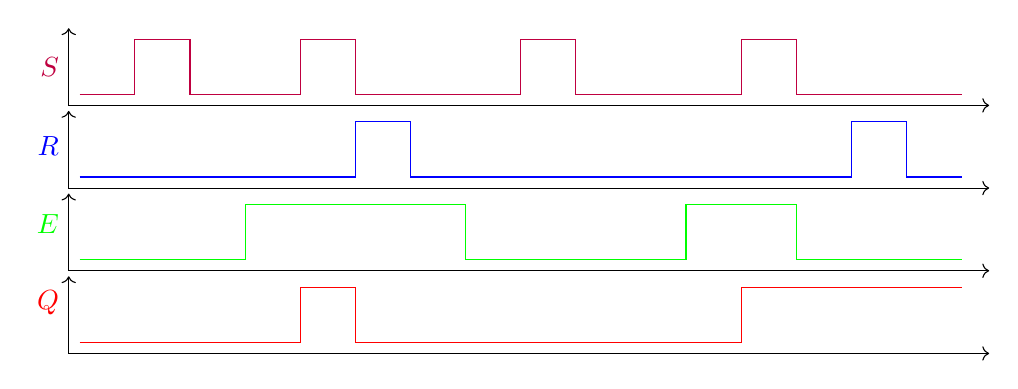
\begin{tikzpicture}[scale=0.7]
        \draw[<->] (-0.2, 1.2) -- (-0.2, -0.2) -- (16.5, -0.2); 
        \draw[<->, yshift=-1.5cm] (-0.2, 1.2) -- (-0.2, -0.2) -- (16.5, -0.2); 
        \draw[<->, yshift=-3cm] (-0.2, 1.2) -- (-0.2, -0.2) -- (16.5, -0.2); 
        \draw[<->, yshift=-4.5cm] (-0.2, 1.2) -- (-0.2, -0.2) -- (16.5, -0.2); 
        \node[purple, left] at (-0.2, 0.5) {$S$}; 
        \node[blue, left, yshift=-1cm] at (-0.2, 0.5) {$R$}; 
        \node[green, left, yshift=-2cm] at (-0.2, 0.5) {$E$}; 
        \node[red, left, yshift=-3cm] at (-0.2, 0.5) {$Q$}; 

        \draw[purple] (0, 0) -- 
          (1, 0) -- (1, 1) -- (2, 1) -- (2, 0) -- 
          (4, 0) -- (4, 1) -- (5, 1) -- (5, 0) -- 
          (8, 0) -- (8, 1) -- (9, 1) -- (9, 0) -- 
          (12, 0) -- (12, 1) -- (13, 1) -- (13, 0) -- 
          (16, 0);
        \draw[blue, yshift=-1.5cm] (0, 0) -- 
          (5, 0) -- (5, 1) -- (6, 1) -- (6, 0) -- 
          (14, 0) -- (14, 1) -- (15, 1) -- (15, 0) -- 
          (16, 0);
        \draw[green, yshift=-3cm] (0, 0) -- 
          (3, 0) -- (3, 1) -- (7, 1) -- (7, 0) -- 
          (11, 0) -- (11, 1) -- (13, 1) -- (13, 0) -- 
          (16, 0);
        \draw[red, yshift=-4.5cm] (0, 0) -- 
          (4, 0) -- (4, 1) -- (5, 1) -- (5, 0) -- 
          (12, 0) -- (12, 1) -- (16, 1);
      \end{tikzpicture}
      \caption{Now we toggle $E$ on and off throughout. We can start off by filling in all the places where $E = 1$, where we want $Q$ to basically copy $S$. At every other place, we just continue what the state $Q$ was in. } 
    \end{figure}
  \end{example}

  Note that we still have the problem of invalid signals. For example, if there was an instance that at the same clock time a signal of $S=1, R=1$ (on either an ungated latch or a gated latch with $E=1$), then both $Q$ and $\overline{Q}$ will be $1$, which will cause both to be $0$, and then $1$, and so on. This causes a race condition, which leads to unpredictable behavior. 

  \begin{figure}[H]
    \centering 
    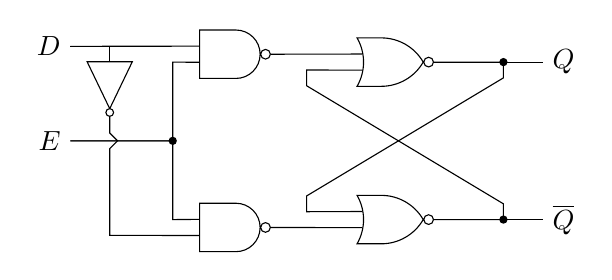
\begin{tikzpicture}[circuit logic US]
      \node[nand gate] (nand1) at (-2, 1.1) {};
      \node[nand gate] (nand2) at (-2, -1.1) {};
      \node[nor gate] (nor1) at (0, 1) {}; 
      \node[nor gate] (nor2) at (0, -1) {}; 
      \node[not gate, point down, scale=0.8] (not1) at (-3.5, 0.8) {};

      \draw (-4, 1.2) -- (nand1.input 1);
      \draw (-4, 1.2) -- (-3.5, 1.2) -- (not1.input); 
      \draw (not1.output) -- (-3.5, 0.1) -- (-3.4, 0) -- (-3.5, -0.1) -- (-3.5, -1.2) -- (nand2.input 2);
      \draw (-4, 0) -- (-2.7, 0) -- (-2.7,1) -- (nand1.input 2);
      \draw (-4, 0) -- (-2.7, 0) -- (-2.7,-1) -- (nand2.input 1);
      \node[left] at (-4,0) {$E$};
      \node[left] at (-4,1.2) {$D$};
      \node[right] at (2, 1) {$Q$};
      \node[right] at (2, -1) {$\overline{Q}$};

      \draw (nand1.output) -- (nor1.input 1);
      \draw (nand2.output) -- (nor2.input 2);
      \draw (nor1.output) -- (2, 1); 
      \draw (nor2.output) -- (2, -1); 

      \draw (nor1.output) -- (1.5, 1) -- (1.5, 0.8) -- (-1, -0.7) -- (-1, -0.9) -- (nor2.input 1);
      \draw (nor2.output) -- (1.5, -1) -- (1.5, -0.8) -- (-1, 0.7) -- (-1, 0.9) -- (nor1.input 2);
      \fill (1.5,1) circle (1.5pt);
      \fill (1.5,-1) circle (1.5pt);
      \fill (-2.7,0) circle (1.5pt);
    \end{tikzpicture} 
    \caption{} 
  \end{figure}

  It turns out that we can simplify this circuit, making it cheaper to produce while still behaving identically. This gives us the D-latch. 

  \begin{definition}[D Latch]
    The \textbf{(gated) data latch (D-latch)} gives us more control over storing a 1-bit in memory. 

    \begin{figure}[H]
      \centering
      \begin{subfigure}[b]{0.48\textwidth}
        \centering
        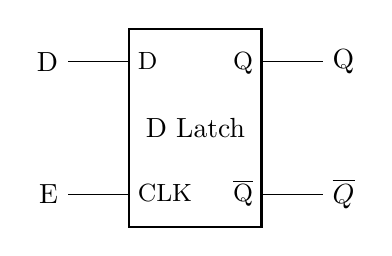
\begin{tikzpicture}
          \node[latch, align=center] (latch) at (0,0) {D Latch};
          \draw (latch.pin 1) -- ++(-0.5,0) node[left] {D};
          \draw (latch.pin 3) -- ++(-0.5,0) node[left] {E};
          \draw (latch.pin 6) -- ++(0.5,0) node[right] {Q};
          \draw (latch.pin 4) -- ++(0.5,0) node[right] {$\overline{Q}$};
        \end{tikzpicture}
        \caption{Chip notation for D latch.}
      \end{subfigure}
      \hfill 
      \begin{subfigure}[b]{0.48\textwidth}
        \centering
          \begin{tabular}{|c|c|c|c|}
            \hline
            $E$ & $D$ & $Q$ & $\overline{Q}$ \\
            \hline
            0 & X & $Q_{\mathrm{prev}}$ & $\overline{Q_{\mathrm{prev}}}$ \\
            \hline
            1 & 0 & 0 & 1 \\
            \hline
            1 & 1 & 1 & 0 \\
            \hline
          \end{tabular}
        \caption{Truth table. Note that the }
      \end{subfigure}
      \caption{}
    \end{figure}

    \begin{figure}[H]
      \centering
      \begin{subfigure}[b]{0.48\textwidth}
        \centering
        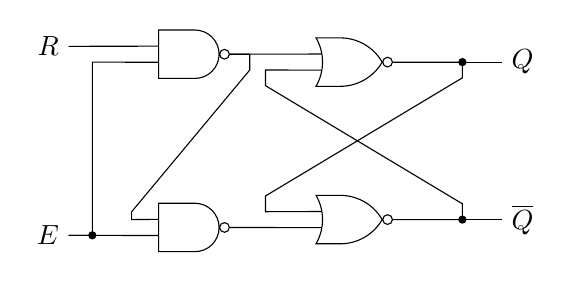
\begin{tikzpicture}[circuit logic US]
          \node[nand gate] (nand1) at (-2, 1.1) {};
          \node[nand gate] (nand2) at (-2, -1.1) {};
          \node[nor gate] (nor1) at (0, 1) {}; 
          \node[nor gate] (nor2) at (0, -1) {}; 

          \draw (-3.5, 1.2) -- (nand1.input 1);
          \draw (-3.5, -1.2) -- (nand2.input 2);
          \node[left] at (-3.5,-1.2) {$E$};
          \node[left] at (-3.5,1.2) {$R$};
          \node[right] at (2, 1) {$Q$};
          \node[right] at (2, -1) {$\overline{Q}$};

          \draw (-3.5, -1.2) -- (-3.2, -1.2) -- (-3.2, 1) -- (nand1.input 2);
          \fill (-3.2, -1.2) circle (1.5pt);
          \draw (nand1.output) -- (-1.2, 1.1) -- (-1.2, 0.9) -- (-2.7, -0.9) -- (-2.7, -1) -- (nand2.input 1);

          \draw (nand1.output) -- (nor1.input 1);
          \draw (nand2.output) -- (nor2.input 2);
          \draw (nor1.output) -- (2, 1); 
          \draw (nor2.output) -- (2, -1); 

          \draw (nor1.output) -- (1.5, 1) -- (1.5, 0.8) -- (-1, -0.7) -- (-1, -0.9) -- (nor2.input 1);
          \draw (nor2.output) -- (1.5, -1) -- (1.5, -0.8) -- (-1, 0.7) -- (-1, 0.9) -- (nor1.input 2);
          \fill (1.5,1) circle (1.5pt);
          \fill (1.5,-1) circle (1.5pt);
        \end{tikzpicture} 
        \caption{Gated XOR SR Latch.}
      \end{subfigure}
      \hfill 
      \begin{subfigure}[b]{0.48\textwidth}
        \centering
        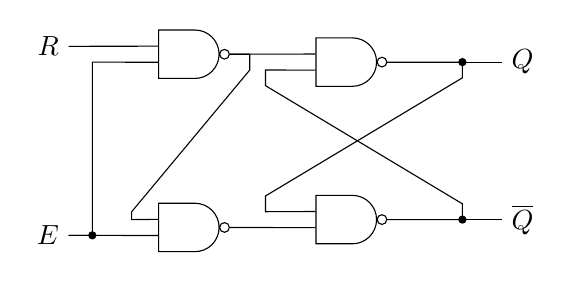
\begin{tikzpicture}[circuit logic US]
          \node[nand gate] (nand1) at (-2, 1.1) {};
          \node[nand gate] (nand2) at (-2, -1.1) {};
          \node[nand gate] (nor1) at (0, 1) {}; 
          \node[nand gate] (nor2) at (0, -1) {}; 

          \draw (-3.5, 1.2) -- (nand1.input 1);
          \draw (-3.5, -1.2) -- (nand2.input 2);
          \node[left] at (-3.5,-1.2) {$E$};
          \node[left] at (-3.5,1.2) {$R$};
          \node[right] at (2, 1) {$Q$};
          \node[right] at (2, -1) {$\overline{Q}$};

          \draw (-3.5, -1.2) -- (-3.2, -1.2) -- (-3.2, 1) -- (nand1.input 2);
          \fill (-3.2, -1.2) circle (1.5pt);
          \draw (nand1.output) -- (-1.2, 1.1) -- (-1.2, 0.9) -- (-2.7, -0.9) -- (-2.7, -1) -- (nand2.input 1);

          \draw (nand1.output) -- (nor1.input 1);
          \draw (nand2.output) -- (nor2.input 2);
          \draw (nor1.output) -- (2, 1); 
          \draw (nor2.output) -- (2, -1); 

          \draw (nor1.output) -- (1.5, 1) -- (1.5, 0.8) -- (-1, -0.7) -- (-1, -0.9) -- (nor2.input 1);
          \draw (nor2.output) -- (1.5, -1) -- (1.5, -0.8) -- (-1, 0.7) -- (-1, 0.9) -- (nor1.input 2);
          \fill (1.5,1) circle (1.5pt);
          \fill (1.5,-1) circle (1.5pt);
        \end{tikzpicture} 
        \caption{Gated NAND SR Latch.}
      \end{subfigure}
      \caption{}
    \end{figure}
  \end{definition}

  \begin{example}[D Latch]
    The essence of the behavior is the output follows the input while $E$ is enabled. 

    \begin{figure}[H]
      \centering 
      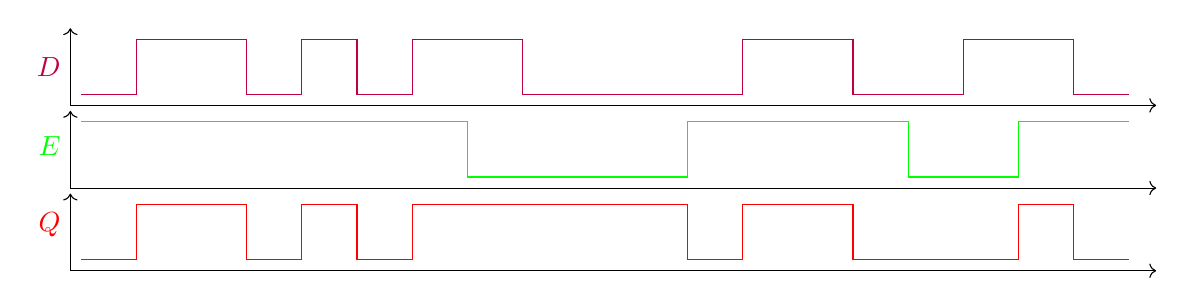
\begin{tikzpicture}[scale=0.7]
        \draw[<->] (-0.2, 1.2) -- (-0.2, -0.2) -- (19.5, -0.2); 
        \draw[<->, yshift=-1.5cm] (-0.2, 1.2) -- (-0.2, -0.2) -- (19.5, -0.2); 
        \draw[<->, yshift=-3cm] (-0.2, 1.2) -- (-0.2, -0.2) -- (19.5, -0.2); 
        \node[purple, left] at (-0.2, 0.5) {$D$}; 
        \node[green, left, yshift=-1cm] at (-0.2, 0.5) {$E$}; 
        \node[red, left, yshift=-2cm] at (-0.2, 0.5) {$Q$}; 

        \draw[purple] (0, 0) -- 
          (1, 0) -- (1, 1) -- (3, 1) -- (3, 0) -- 
          (4, 0) -- (4, 1) -- (5, 1) -- (5, 0) -- 
          (6, 0) -- (6, 1) -- (8, 1) -- (8, 0) -- 
          (12, 0) -- (12, 1) -- (14, 1) -- (14, 0) -- 
          (16, 0) -- (16, 1) -- (18, 1) -- (18, 0) -- 
          (19, 0);
        \draw[green, yshift=-1.5cm] 
          (0, 1) --  (7, 1) -- (7, 0) -- 
          (11, 0) -- (11, 1) -- (15, 1) -- (15, 0) -- 
          (17, 0) -- (17, 1) -- (19, 1);
        \draw[red, yshift=-3cm] (0, 0) -- 
          (1, 0) -- (1, 1) -- (3, 1) -- (3, 0) -- 
          (4, 0) -- (4, 1) -- (5, 1) -- (5, 0) -- 
          (6, 0) -- (6, 1) -- (11, 1) -- (11, 0) -- 
          (12, 0) -- (12, 1) -- (14, 1) -- (14, 0) -- 
          (17, 0) -- (17, 1) -- (18, 1) -- (18, 0) -- 
          (19, 0);
      \end{tikzpicture}
      \caption{Again, we just let the result $Q$ follow the input $D$ whenever $E = 1$,and continue the rest for when $E = 0$.}
    \end{figure}
  \end{example} 

  Therefore, if we want to store a bit of information, we set $E = 1$, collect that bit from $D$, and then set $E = 0$ to latch it in place. 

\subsection{Clocked Latches}

  This behavior is quite stable for storing 1-bit, but we need more control when storing a multi-bit buffer, where we need several D-latches working in tandem. The general idea is that if we have a multi-bit buffer, we want a set of D-latches to be enabled and disabled at once. 

  \begin{figure}[H]
    \centering 
    \begin{tikzpicture}
      \foreach \h in {0, 2, 4} {
        \draw (0, 0+\h) rectangle (0.8, 1.2+\h);
        \draw (-3, 1+\h) -- (0, 1+\h); 
        \draw (0.8, 0.65+\h) -- (2, 0.65+\h); 
        \node[right, font=\footnotesize] at (0, 1+\h) {$D$};
        \node[left, font=\footnotesize] at (0.8, 0.65+\h) {$Q$};
        \node[right, font=\footnotesize] at (0, 0.3+\h) {$E$};
        \draw (-1, 0.3+\h) -- (0, 0.3+\h);
        \fill (-1, 0.3+\h) circle (1.5pt);
      }
      \node[draw, circle] (clock) at (-4, -1) {clock};
      \draw (clock.east) -- (-1, -1) -- (-1, 4.3);
    \end{tikzpicture}
    \caption{Multiple D-latches enabled and disabled by some external source. The system clock would be a good candidate.} 
  \end{figure}

  Therefore, given the system clock, our waveforms would look like this. 

  \begin{figure}[H]
    \centering 
    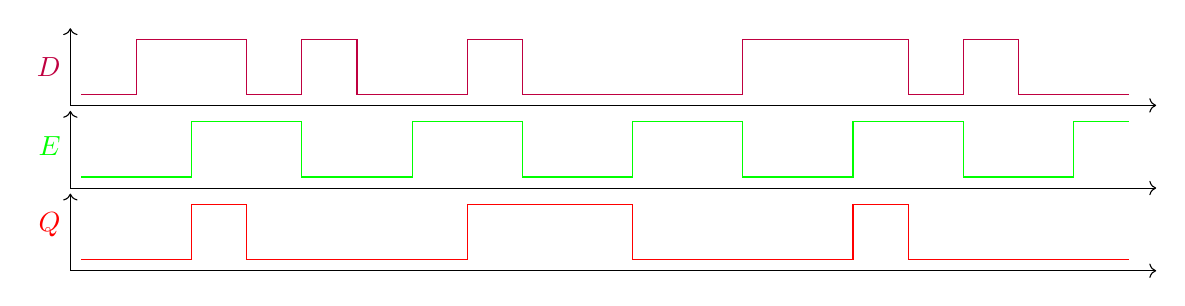
\begin{tikzpicture}[scale=0.7]
      \draw[<->] (-0.2, 1.2) -- (-0.2, -0.2) -- (19.5, -0.2); 
      \draw[<->, yshift=-1.5cm] (-0.2, 1.2) -- (-0.2, -0.2) -- (19.5, -0.2); 
      \draw[<->, yshift=-3cm] (-0.2, 1.2) -- (-0.2, -0.2) -- (19.5, -0.2); 
      \node[purple, left] at (-0.2, 0.5) {$D$}; 
      \node[green, left, yshift=-1cm] at (-0.2, 0.5) {$E$}; 
      \node[red, left, yshift=-2cm] at (-0.2, 0.5) {$Q$}; 

      \draw[purple] (0, 0) -- 
        (1, 0) -- (1, 1) -- (3, 1) -- (3, 0) -- 
        (4, 0) -- (4, 1) -- (5, 1) -- (5, 0) -- 
        (7, 0) -- (7, 1) -- (8, 1) -- (8, 0) -- 
        (12, 0) -- (12, 1) -- (15, 1) -- (15, 0) -- 
        (16, 0) -- (16, 1) -- (17, 1) -- (17, 0) -- 
        (19, 0);
      \draw[green, yshift=-1.5cm] (0, 0) -- 
        (2, 0) -- (2, 1) -- (4, 1) -- (4, 0) -- 
        (6, 0) -- (6, 1) -- (8, 1) -- (8, 0) -- 
        (10, 0) -- (10, 1) -- (12, 1) -- (12, 0) -- 
        (14, 0) -- (14, 1) -- (16, 1) -- (16, 0) -- 
        (18, 0) -- (18, 1) -- (19, 1);
      \draw[red, yshift=-3cm] (0, 0) -- 
        (2, 0) -- (2, 1) -- (3, 1) -- (3, 0) -- 
        (7, 0) -- (7, 1) -- (10, 1) -- (10, 0) -- 
        (14, 0) -- (14, 1) -- (15, 1) -- (15, 0) -- 
        (19, 0);
    \end{tikzpicture}
    \caption{$E$ is connected to a clock that ocsillates at regular intervals.}
  \end{figure}

  This is still not a perfect solution for synchronizing some components. Depending on the frequency of the clock, $E$ may be high for as long at 50 microseconds. That's a long time for the data latch to be open to changes in $D$. For some applications, particularly those where the outputs are fed back to the inputs, we can avoid disorder and noise from $D$ by drastically limiting the amount of time $E$ is open during each clock cycle. 
  
  But simply increasing the frequency of the clock isn't a practical solution, given that a computer contains a mixture of fast and slow components. A more clever solution is to only allow changes to the latch when the clock input $E$ is changing from low to high. Due to propagation delay, this is indeed a feasible solution since the waveforms are not truly square waves. 

  \begin{definition}[Rising, Falling Edge]
    The period when a signal 
    \begin{enumerate}
      \item changes from $0$ to $1$ is called the \textbf{rising edge}. 
      \item changes from $1$ to $0$ is called the \textbf{falling edge}. 
    \end{enumerate}
    This usually takes a few nanoseconds. 

    \begin{figure}[H]
      \centering 
      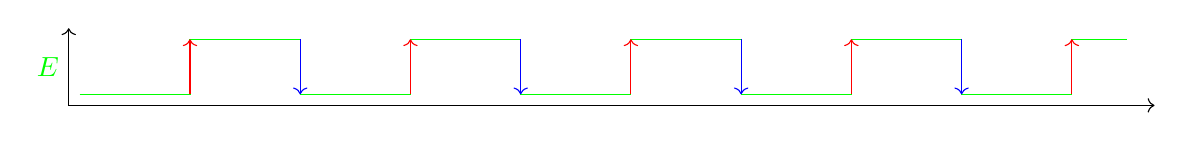
\begin{tikzpicture}[scale=0.7]
        \draw[<->] (-0.2, 1.2) -- (-0.2, -0.2) -- (19.5, -0.2); 
        \node[green, left] at (-0.2, 0.5) {$E$}; 

        \draw[green] (0, 0) -- 
          (2, 0) -- (2, 1) -- (4, 1) -- (4, 0) -- 
          (6, 0) -- (6, 1) -- (8, 1) -- (8, 0) -- 
          (10, 0) -- (10, 1) -- (12, 1) -- (12, 0) -- 
          (14, 0) -- (14, 1) -- (16, 1) -- (16, 0) -- 
          (18, 0) -- (18, 1) -- (19, 1);

        \draw[blue, <-] (4, 0) -- (4, 1); 
        \draw[blue, <-] (8, 0) -- (8, 1); 
        \draw[blue, <-] (12, 0) -- (12, 1); 
        \draw[blue, <-] (16, 0) -- (16, 1); 

        \draw[red, ->] (2, 0) -- (2, 1); 
        \draw[red, ->] (6, 0) -- (6, 1); 
        \draw[red, ->] (10, 0) -- (10, 1); 
        \draw[red, ->] (14, 0) -- (14, 1); 
        \draw[red, ->] (18, 0) -- (18, 1); 
      \end{tikzpicture}
      \caption{Rising edges are in red, falling edges in blue.}
    \end{figure}
  \end{definition}

  We want to build a D-latch that will respond to changes in $D$ \textit{at the rising edge}, with subsequent changes in $D$ being ignored until the next rising edge. 

  \begin{figure}[H]
    \centering
    \begin{subfigure}[b]{0.32\textwidth}
      \centering
      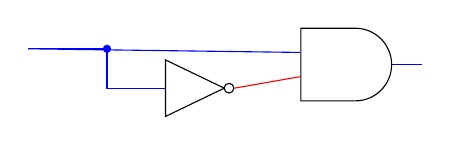
\begin{tikzpicture}[circuit logic US]
        \node[and gate, scale=1.5] (and) at (3, 0) {};
        \node[not gate] (not) at (1, -0.3) {};
        \draw[blue] (-1, 0.2) -- (0, 0.2) -- (0, -0.3) -- (not.input);
        \draw[red] (not.output) -- (and.input 2); 
        \draw[blue] (-1, 0.2) -- (and.input 1); 
        \draw[blue] (and.output) -- (4, 0);
        \fill[blue] (0, 0.2) circle (1.5pt);
      \end{tikzpicture}
      \caption{By default the input current is $0$, and so the top input of the AND gate is $0$ and the bottom is $1$. }
    \end{subfigure}
    \hfill 
    \begin{subfigure}[b]{0.32\textwidth}
      \centering
      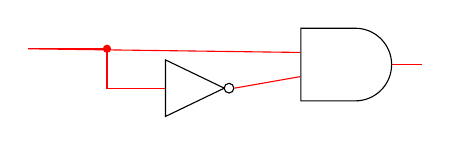
\begin{tikzpicture}[circuit logic US]
        \node[and gate, scale=1.5] (and) at (3, 0) {};
        \node[not gate] (not) at (1, -0.3) {};
        \draw[red] (-1, 0.2) -- (0, 0.2) -- (0, -0.3) -- (not.input);
        \draw[red] (not.output) -- (and.input 2); 
        \draw[red] (-1, 0.2) -- (and.input 1); 
        \draw[red] (and.output) -- (4, 0);
        \fill[red] (0, 0.2) circle (1.5pt);
      \end{tikzpicture}
      \caption{If the electric current of $1$ travels through the input wire, the top AND input becomes $1$. There is a small delay where the current does not reach the output of the NOT gate, so the output is $1$. }
    \end{subfigure}
    \hfill 
    \begin{subfigure}[b]{0.32\textwidth}
      \centering
      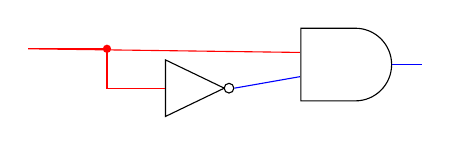
\begin{tikzpicture}[circuit logic US]
        \node[and gate, scale=1.5] (and) at (3, 0) {};
        \node[not gate] (not) at (1, -0.3) {};
        \draw[red] (-1, 0.2) -- (0, 0.2) -- (0, -0.3) -- (not.input);
        \draw[blue] (not.output) -- (and.input 2); 
        \draw[red] (-1, 0.2) -- (and.input 1); 
        \draw[blue] (and.output) -- (4, 0);
        \fill[red] (0, 0.2) circle (1.5pt);
      \end{tikzpicture}
      \caption{The signal goes through the NOT gate, turning the AND output back to $0$.}
    \end{subfigure}
    \caption{An edge detection device. Note that if we want to delay the signal even further, we can put an arbitrary amount of NAND gates.}
  \end{figure}

  We take this idea to build an edge detection device. 

  \begin{definition}[Edge Detection Device]
    This is a rising edge detection device. Note that depending on many factors, like manufacturing, temperature, etc., there may not be a long enough delay to actually detect an edge, and in this case you can just add more (odd number of ) NOT gates 

    \begin{figure}[H]
      \centering
      \begin{subfigure}[b]{0.48\textwidth}
        \centering
        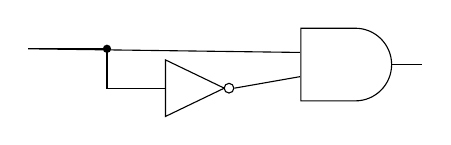
\begin{tikzpicture}[circuit logic US]
          \node[and gate, scale=1.5] (and) at (3, 0) {};
          \node[not gate] (not) at (1, -0.3) {};
          \draw (-1, 0.2) -- (0, 0.2) -- (0, -0.3) -- (not.input);
          \draw (not.output) -- (and.input 2); 
          \draw (-1, 0.2) -- (and.input 1); 
          \draw (and.output) -- (4, 0);
          \fill (0, 0.2) circle (1.5pt);
        \end{tikzpicture}
        \caption{Positive edge triggered detection device.}
      \end{subfigure}
      \hfill 
      \begin{subfigure}[b]{0.48\textwidth}
        \centering
        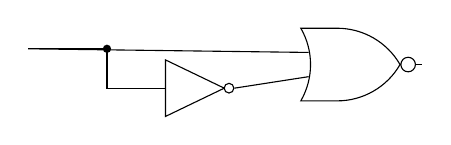
\begin{tikzpicture}[circuit logic US]
          \node[nor gate, scale=1.5] (and) at (3, 0) {};
          \node[not gate] (not) at (1, -0.3) {};
          \draw (-1, 0.2) -- (0, 0.2) -- (0, -0.3) -- (not.input);
          \draw (not.output) -- (and.input 2); 
          \draw (-1, 0.2) -- (and.input 1); 
          \draw (and.output) -- (4, 0);
          \fill (0, 0.2) circle (1.5pt);
        \end{tikzpicture}
        \caption{Negative edge triggered detection device.}
      \end{subfigure}
      \caption{}
    \end{figure}

    It has the following waveform. 

    \begin{figure}[H]
      \centering 
      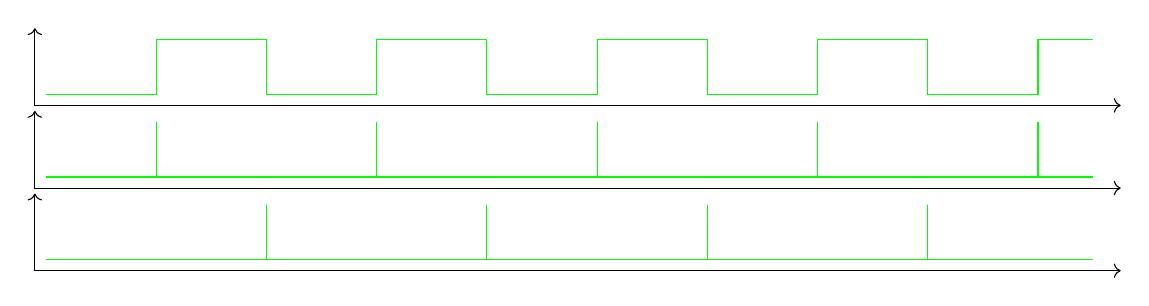
\begin{tikzpicture}[scale=0.7]
        \draw[<->] (-0.2, 1.2) -- (-0.2, -0.2) -- (19.5, -0.2); 
        \draw[<->, yshift=-1.5cm] (-0.2, 1.2) -- (-0.2, -0.2) -- (19.5, -0.2); 
        \draw[<->, yshift=-3cm] (-0.2, 1.2) -- (-0.2, -0.2) -- (19.5, -0.2); 

        \draw[green] (0, 0) -- 
          (2, 0) -- (2, 1) -- (4, 1) -- (4, 0) -- 
          (6, 0) -- (6, 1) -- (8, 1) -- (8, 0) -- 
          (10, 0) -- (10, 1) -- (12, 1) -- (12, 0) -- 
          (14, 0) -- (14, 1) -- (16, 1) -- (16, 0) -- 
          (18, 0) -- (18, 1) -- (19, 1);

        \draw[green, yshift=-1.5cm] (0, 0) -- 
          (2, 0) -- (2, 1) -- (2, 1) -- (2, 0) -- 
          (6, 0) -- (6, 1) -- (6, 1) -- (6, 0) -- 
          (10, 0) -- (10, 1) -- (10, 1) -- (10, 0) -- 
          (14, 0) -- (14, 1) -- (14, 1) -- (14, 0) -- 
          (18, 0) -- (18, 1) -- (18, 1) -- (18, 0) -- 
          (19, 0);

        \draw[green, yshift=-3cm] (0, 0) -- 
          (4, 0) -- (4, 1) -- (4, 0) -- 
          (8, 0) -- (8, 1) -- (8, 0) -- 
          (12, 0) -- (12, 1) -- (12, 0) -- 
          (16, 0) -- (16, 1) -- (16, 0) -- 
          (19, 0);
      \end{tikzpicture}
      \caption{The clock cycle (top). Positive edge detection device (middle). Negative edge detection device (bottom). }
    \end{figure}
  \end{definition}

  Now if we combine our D latch with the edge detection device, we change it from a level-triggered device to an edge-triggered device. Since we are using a clock as our trigger, we also call this a \textit{clocked D-latch}. 

  \begin{definition}[Clocked D Latch]
    A \textbf{clocked D latch}, also called an \textbf{edge-triggered D-latch},\footnote{Sometimes, this is referred to as a flip flop, but we will distinguish that a bit later.} is a D-latch that is enabled on the rising edge of a clock cycle. 

    \begin{figure}[H]
      \centering 
      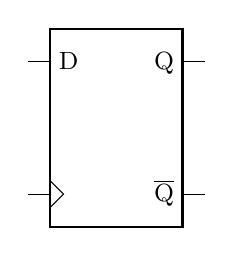
\begin{tikzpicture}[circuit logic US]
        \node[flipflop D] (D1){};
      \end{tikzpicture}
      \caption{A pulse D latch. Note that the triangle is used to indicate that the clock is inputted. } 
    \end{figure}

    \begin{figure}[H]
      \centering 
      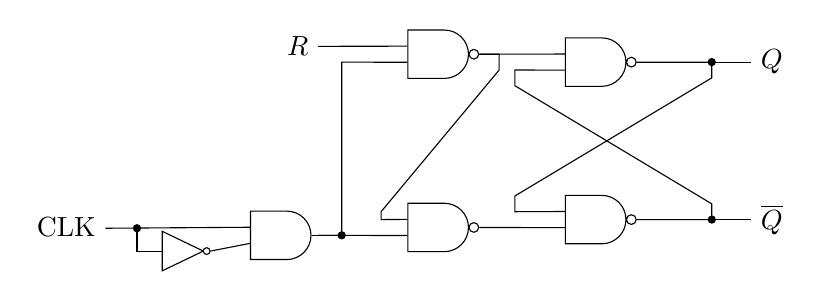
\begin{tikzpicture}[circuit logic US]
        \node[and gate] (and) at (-4, -1.2) {};
        \node[not gate, scale=0.7] (not) at (-5.3, -1.4) {};
        \draw (-6.2, -1.11) -- (and.input 1);
        \draw (-5.8, -1.11) -- (-5.8, -1.4) -- (not.input);
        \fill (-5.8, -1.11) circle (1.5pt); 
        \node[left] at (-6.2, -1.1) {CLK}; 
        \draw(and.output) -- (-3.2, -1.2);
        \draw(not.output) -- (and.input 2); 

        \node[nand gate] (nand1) at (-2, 1.1) {};
        \node[nand gate] (nand2) at (-2, -1.1) {};
        \node[nand gate] (nor1) at (0, 1) {}; 
        \node[nand gate] (nor2) at (0, -1) {}; 

        \draw (-3.5, 1.2) -- (nand1.input 1);
        \draw (-3.5, -1.2) -- (nand2.input 2);
        \node[left] at (-3.5,1.2) {$R$};
        \node[right] at (2, 1) {$Q$};
        \node[right] at (2, -1) {$\overline{Q}$};

        \draw (-3.5, -1.2) -- (-3.2, -1.2) -- (-3.2, 1) -- (nand1.input 2);
        \fill (-3.2, -1.2) circle (1.5pt);
        \draw (nand1.output) -- (-1.2, 1.1) -- (-1.2, 0.9) -- (-2.7, -0.9) -- (-2.7, -1) -- (nand2.input 1);

        \draw (nand1.output) -- (nor1.input 1);
        \draw (nand2.output) -- (nor2.input 2);
        \draw (nor1.output) -- (2, 1); 
        \draw (nor2.output) -- (2, -1); 

        \draw (nor1.output) -- (1.5, 1) -- (1.5, 0.8) -- (-1, -0.7) -- (-1, -0.9) -- (nor2.input 1);
        \draw (nor2.output) -- (1.5, -1) -- (1.5, -0.8) -- (-1, 0.7) -- (-1, 0.9) -- (nor1.input 2);
        \fill (1.5,1) circle (1.5pt);
        \fill (1.5,-1) circle (1.5pt);
      \end{tikzpicture} 
      \caption{} 
    \end{figure}
  \end{definition}

  \begin{example}[Clocked D Latch Waveforms]
    \begin{figure}[H]
      \centering 
      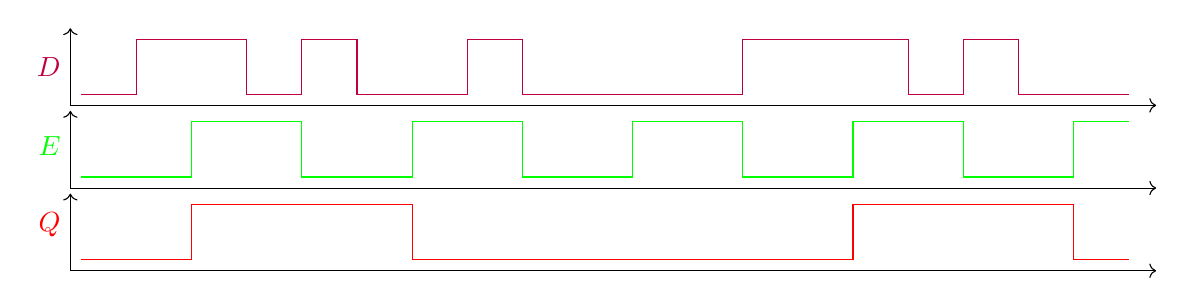
\begin{tikzpicture}[scale=0.7]
        \draw[<->] (-0.2, 1.2) -- (-0.2, -0.2) -- (19.5, -0.2); 
        \draw[<->, yshift=-1.5cm] (-0.2, 1.2) -- (-0.2, -0.2) -- (19.5, -0.2); 
        \draw[<->, yshift=-3cm] (-0.2, 1.2) -- (-0.2, -0.2) -- (19.5, -0.2); 
        \node[purple, left] at (-0.2, 0.5) {$D$}; 
        \node[green, left, yshift=-1cm] at (-0.2, 0.5) {$E$}; 
        \node[red, left, yshift=-2cm] at (-0.2, 0.5) {$Q$}; 

        \draw[purple] (0, 0) -- 
          (1, 0) -- (1, 1) -- (3, 1) -- (3, 0) -- 
          (4, 0) -- (4, 1) -- (5, 1) -- (5, 0) -- 
          (7, 0) -- (7, 1) -- (8, 1) -- (8, 0) -- 
          (12, 0) -- (12, 1) -- (15, 1) -- (15, 0) -- 
          (16, 0) -- (16, 1) -- (17, 1) -- (17, 0) -- 
          (19, 0);
        \draw[green, yshift=-1.5cm] (0, 0) -- 
          (2, 0) -- (2, 1) -- (4, 1) -- (4, 0) -- 
          (6, 0) -- (6, 1) -- (8, 1) -- (8, 0) -- 
          (10, 0) -- (10, 1) -- (12, 1) -- (12, 0) -- 
          (14, 0) -- (14, 1) -- (16, 1) -- (16, 0) -- 
          (18, 0) -- (18, 1) -- (19, 1);
        \draw[red, yshift=-3cm] (0, 0) -- 
          (2, 0) -- (2, 1) -- (6, 1) -- (6, 0) -- 
          (14, 0) -- (14, 1) -- (18, 1) -- (18, 0) --
          (19, 0);
      \end{tikzpicture}
      \caption{Again, we just let the result $Q$ follow the input $D$ whenever $E = 1$,and continue the rest for when $E = 0$.}
    \end{figure}
  \end{example}

  \begin{definition}[Pulse Latch]
    Another enhancement we can make is to have an option to manually set the latch to be either $Q = 1$ or $0$, independent of the clock. This gives us the \textbf{pulse D-latch}, which allows us to initialize it unconditionally. 

    \begin{figure}[H]
      \centering 
      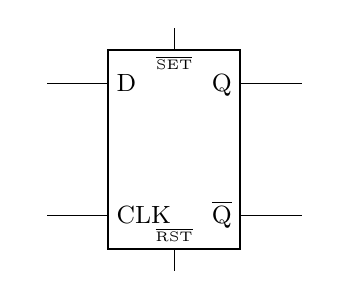
\begin{tikzpicture}
        \node[latch, align=center, add async SR] (latch) at (0,0) {};
        \draw (latch.pin 1) -- ++(-0.5,0) node[left] {};
        \draw (latch.pin 3) -- ++(-0.5,0) node[left] {};
        \draw (latch.pin 6) -- ++(0.5,0) node[right] {};
        \draw (latch.pin 4) -- ++(0.5,0) node[right] {};
      \end{tikzpicture}
      \caption{D latch with asynchronous set/reset.} 
    \end{figure}

    The implementation is to simply add extra inputs after the NAND gates. 

    \begin{figure}[H]
      \centering 
      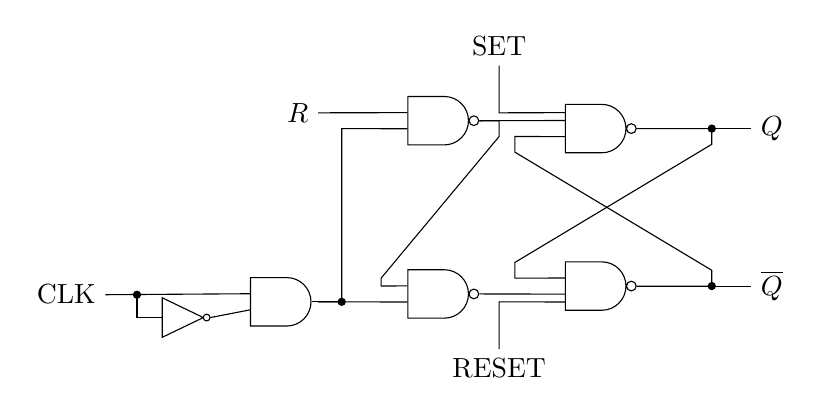
\begin{tikzpicture}[circuit logic US]
        \node[and gate] (and) at (-4, -1.2) {};
        \node[not gate, scale=0.7] (not) at (-5.3, -1.4) {};
        \draw (-6.2, -1.11) -- (and.input 1);
        \draw (-5.8, -1.11) -- (-5.8, -1.4) -- (not.input);
        \fill (-5.8, -1.11) circle (1.5pt); 
        \node[left] at (-6.2, -1.1) {CLK}; 
        \draw(and.output) -- (-3.2, -1.2);
        \draw(not.output) -- (and.input 2); 

        \node[nand gate] (nand1) at (-2, 1.1) {};
        \node[nand gate] (nand2) at (-2, -1.1) {};
        \node[nand gate, number inputs=3] (nor1) at (0, 1) {}; 
        \node[nand gate, number inputs=3] (nor2) at (0, -1) {}; 

        \draw (-3.5, 1.2) -- (nand1.input 1);
        \draw (-3.5, -1.2) -- (nand2.input 2);
        \node[left] at (-3.5,1.2) {$R$};
        \node[right] at (2, 1) {$Q$};
        \node[right] at (2, -1) {$\overline{Q}$};

        \draw (-3.5, -1.2) -- (-3.2, -1.2) -- (-3.2, 1) -- (nand1.input 2);
        \fill (-3.2, -1.2) circle (1.5pt);
        \draw (nand1.output) -- (-1.2, 1.1) -- (-1.2, 0.9) -- (-2.7, -0.9) -- (-2.7, -1) -- (nand2.input 1);

        \node[above] at (-1.2, 1.8) {SET};
        \node[below] at (-1.2, -1.8) {RESET};
        \draw (-1.2, 1.8) -- (-1.2, 1.2) -- ([yshift=0.1cm]nor1.input 1);
        \draw (-1.2, -1.8) -- (-1.2, -1.2) -- ([yshift=-0.1cm]nor2.input 2);
        \draw (nand1.output) -- (nor1.input 1);
        \draw (nand2.output) -- (nor2.input 2);
        \draw (nor1.output) -- (2, 1); 
        \draw (nor2.output) -- (2, -1); 

        \draw (nor1.output) -- (1.5, 1) -- (1.5, 0.8) -- (-1, -0.7) -- (-1, -0.9) -- (nor2.input 1);
        \draw (nor2.output) -- (1.5, -1) -- (1.5, -0.8) -- (-1, 0.7) -- (-1, 0.9) -- (nor1.input 2);
        \fill (1.5,1) circle (1.5pt);
        \fill (1.5,-1) circle (1.5pt);
      \end{tikzpicture} 
      \caption{} 
    \end{figure}
  \end{definition}

  This gives us a reliable device for storing 1 bit of memory. It is enabled and disabled by a clock signal, and used in registers, memory circuits, and counters as we will see later. 

\subsection{Flip Flops}

  So far, we have considered various mechanisms that allowed for greater control of a latch, along with robustness to noise. Now we revisit the final problem of attempting to \textit{coordinate} a group of latches, where timing is a fundamental consideration. Just like the conductor of an orchestra, the clock sets the timing and the pace of everything in the computer, which consists of both fast and slow moving parts. 

  \begin{figure}[H]
    \centering 
    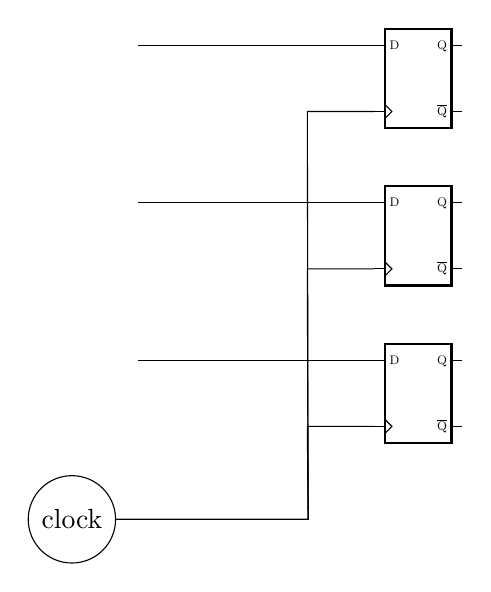
\begin{tikzpicture}
      \node[draw, circle] (clock) at (-4, -1) {clock};
      \foreach \h in {0, 2, 4} {
        \node[flipflop D, scale=0.5] (D1) at (0.4, 0.6+\h){};
        \draw (D1.pin 3) -- ++(-0.85, 0) -- (-1, -1) -- (clock.east);
        \draw (D1.pin 1) -- ++ (-3, 0);
      }
    \end{tikzpicture}
    \caption{}
  \end{figure}

  Ideally, to synchronize the setting of these latches we'd make all of the inputs the way we want them to be while the clock signal is low. Then, when the clock signal becomes high, these input values would be transmitted to the latches and their values stored. 

  But unwanted fluctuations---known as \textit{glitches}---can occur on the data lines because of propagation delays and even noise.  Conceivably, we can have a situation in which our latches haven't had enough time to achieve their correct values before the clock pulse ends. It is crucial that these inputs are allowed to settle into their correct values while the clock signal is high. This is because there is a different circuit ready to make iemmediate use of the data in the register, even perhaps during the very next clock cycle. The outputs of these latches have to be stable before they are sampled. The data in this register must be accurate before something else reads it. Otherwise, we would have complete garbage outputs. 

  We could try to avoid the problem caused by glitches by speeding up the clock, allowing less time for them to matter, but we also have to allow time for the components to do their jobs. We have to cater for their propagation delays. If a clock is running too quickly, some components won't be able to keep up. 

  We can also make circuits less susceptible to glitches by building edge-triggered devices like pulse latches, but the rising edge of a clock cycle is only in the order of a few nanoseconds, and even with very careful design, there might not be enough time for everything to keep pace. Therefore, the clock period must be so that all of the other circuits have time to stabilize during the same high phase of the same clock cycle. 

  Ultimately, if all circuits in a computer work on the basis that only one signal change per clock cycle matters, then their behavior can be coordinate reliably. One way that we can ensure that this is the case is to build a memory device that is immune to glitches, called the \textit{master-slave D-type flip-flop}. With this, we can precisely control the moment at which a group of them will change state. 

  \begin{definition}[Master-Slave D-Type Flip Flop]
    The \textbf{master-slave D-Type flip-flop (DFF)} consists of two active-high gated latches. The left portion, called the \textit{master}, is a gated D-latch. The right portion, called the \textit{slave}, is a gated SR latch that takes the output of the master as its input and is enabled by the inverse of the clock signal. 

    Taken together, the data and the clock inputs enable to the DFF to implement the time-based behavior 
    \begin{equation}
      \mathrm{out}(t) = \mathrm{in}(t - 1) 
    \end{equation}
    That is, the DFF outputs the input value from the previous time unit. 

    \begin{figure}[H]
      \centering 
      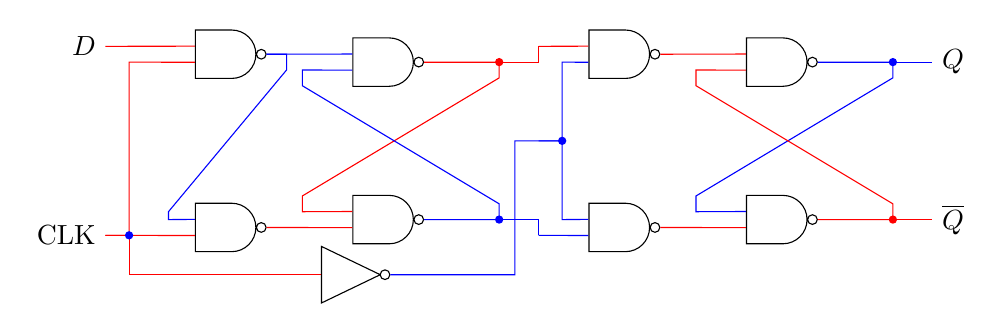
\begin{tikzpicture}[circuit logic US]
        \begin{scope}[xshift=5cm]
          \node[nand gate] (nand13) at (-2, 1.1) {};
          \node[nand gate] (nand24) at (-2, -1.1) {};
          \node[nand gate] (nand14) at (0, 1) {}; 
          \node[nand gate] (nand23) at (0, -1) {}; 
          \node[not gate] (not) at (-5.5, -1.7) {}; 
          \draw[red] (-3, 1.2) -- (nand13.input 1);
          \draw[blue] (-3, -1.2) -- (nand24.input 2);
          \draw[red] (-8.2, -1.2) -- (-8.2, -1.7) -- (not.input); 
          \draw[blue] (not.output) -- (-3.3, -1.7) -- (-3.3, 0) -- (-2.7, 0) -- (-2.7,1) -- (nand13.input 2);
          
          \draw[blue] (-3, 0) -- (-2.7, 0) -- (-2.7,-1) -- (nand24.input 1);
          \node[right] at (2, 1) {$Q$};
          \node[right] at (2, -1) {$\overline{Q}$};
          \draw[red] (nand13.output) -- (nand14.input 1);
          \draw[red] (nand24.output) -- (nand23.input 2);
          \draw[blue] (nand14.output) -- (2, 1); 
          \draw[red] (nand23.output) -- (2, -1); 
          \draw[blue] (nand14.output) -- (1.5, 1) -- (1.5, 0.8) -- (-1, -0.7) -- (-1, -0.9) -- (nand23.input 1);
          \draw[red] (nand23.output) -- (1.5, -1) -- (1.5, -0.8) -- (-1, 0.7) -- (-1, 0.9) -- (nand14.input 2);
          \fill[blue] (1.5,1) circle (1.5pt);
          \fill[red] (1.5,-1) circle (1.5pt);
          \fill[blue] (-2.7,0) circle (1.5pt);
        \end{scope}

        \node[nand gate] (nand1) at (-2, 1.1) {};
        \node[nand gate] (nand2) at (-2, -1.1) {};
        \node[nand gate] (nor1) at (0, 1) {}; 
        \node[nand gate] (nor2) at (0, -1) {}; 

        \draw[red] (-3.5, 1.2) -- (nand1.input 1);
        \draw[red] (-3.5, -1.2) -- (nand2.input 2);
        \node[left] at (-3.5,-1.2) {CLK};
        \node[left] at (-3.5,1.2) {$D$};

        \draw[red] (-3.5, -1.2) -- (-3.2, -1.2) -- (-3.2, 1) -- (nand1.input 2);
        \fill[blue] (-3.2, -1.2) circle (1.5pt);
        \draw[blue] (nand1.output) -- (-1.2, 1.1) -- (-1.2, 0.9) -- (-2.7, -0.9) -- (-2.7, -1) -- (nand2.input 1);

        \draw[blue] (nand1.output) -- (nor1.input 1);
        \draw[red] (nand2.output) -- (nor2.input 2);
        \draw[red] (nor1.output) -- (2, 1) -- (2, 1.2); 
        \draw[blue] (nor2.output) -- (2, -1) -- (2, -1.2); 

        \draw[red] (nor1.output) -- (1.5, 1) -- (1.5, 0.8) -- (-1, -0.7) -- (-1, -0.9) -- (nor2.input 1);
        \draw[blue] (nor2.output) -- (1.5, -1) -- (1.5, -0.8) -- (-1, 0.7) -- (-1, 0.9) -- (nor1.input 2);
        \fill[red] (1.5,1) circle (1.5pt);
        \fill[blue] (1.5,-1) circle (1.5pt);
      \end{tikzpicture} 
      \caption{The master reads the input value $D$ when the clock signal is high (or more specifically, the rising edge of the clock cycle) and latches onto it. Meanwhile, the slave is disabled, so the new output from the flip flop is not available just yet. } 
    \end{figure}

    \begin{figure}[H]
      \centering 
      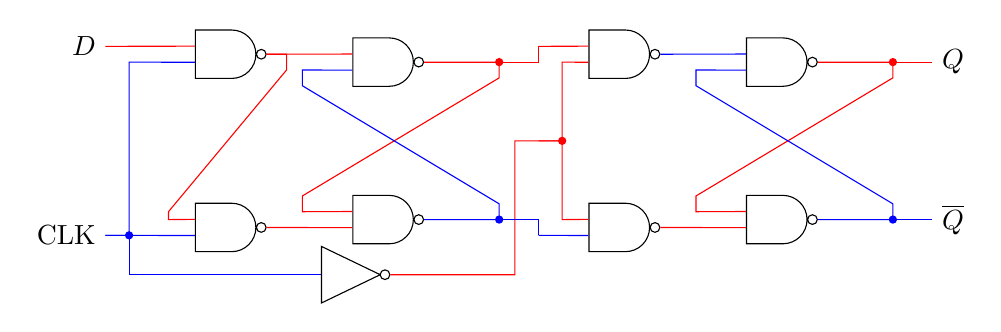
\begin{tikzpicture}[circuit logic US]
        \begin{scope}[xshift=5cm]
          \node[nand gate] (nand13) at (-2, 1.1) {};
          \node[nand gate] (nand24) at (-2, -1.1) {};
          \node[nand gate] (nand14) at (0, 1) {}; 
          \node[nand gate] (nand23) at (0, -1) {}; 
          \node[not gate] (not) at (-5.5, -1.7) {}; 
          \draw[red] (-3, 1.2) -- (nand13.input 1);
          \draw[blue] (-3, -1.2) -- (nand24.input 2);
          \draw[blue] (-8.2, -1.2) -- (-8.2, -1.7) -- (not.input); 
          \draw[red] (not.output) -- (-3.3, -1.7) -- (-3.3, 0) -- (-2.7, 0) -- (-2.7,1) -- (nand13.input 2);
          
          \draw[red] (-3, 0) -- (-2.7, 0) -- (-2.7,-1) -- (nand24.input 1);
          \node[right] at (2, 1) {$Q$};
          \node[right] at (2, -1) {$\overline{Q}$};
          \draw[blue] (nand13.output) -- (nand14.input 1);
          \draw[red] (nand24.output) -- (nand23.input 2);
          \draw[red] (nand14.output) -- (2, 1); 
          \draw[blue] (nand23.output) -- (2, -1); 
          \draw[red] (nand14.output) -- (1.5, 1) -- (1.5, 0.8) -- (-1, -0.7) -- (-1, -0.9) -- (nand23.input 1);
          \draw[blue] (nand23.output) -- (1.5, -1) -- (1.5, -0.8) -- (-1, 0.7) -- (-1, 0.9) -- (nand14.input 2);
          \fill[red] (1.5,1) circle (1.5pt);
          \fill[blue] (1.5,-1) circle (1.5pt);
          \fill[red] (-2.7,0) circle (1.5pt);
        \end{scope}

        \node[nand gate] (nand1) at (-2, 1.1) {};
        \node[nand gate] (nand2) at (-2, -1.1) {};
        \node[nand gate] (nor1) at (0, 1) {}; 
        \node[nand gate] (nor2) at (0, -1) {}; 

        \draw[red] (-3.5, 1.2) -- (nand1.input 1);
        \draw[blue] (-3.5, -1.2) -- (nand2.input 2);
        \node[left] at (-3.5,-1.2) {CLK};
        \node[left] at (-3.5,1.2) {$D$};

        \draw[blue] (-3.5, -1.2) -- (-3.2, -1.2) -- (-3.2, 1) -- (nand1.input 2);
        \fill[blue] (-3.2, -1.2) circle (1.5pt);
        \draw[red] (nand1.output) -- (-1.2, 1.1) -- (-1.2, 0.9) -- (-2.7, -0.9) -- (-2.7, -1) -- (nand2.input 1);

        \draw[red] (nand1.output) -- (nor1.input 1);
        \draw[red] (nand2.output) -- (nor2.input 2);
        \draw[red] (nor1.output) -- (2, 1) -- (2, 1.2); 
        \draw[blue] (nor2.output) -- (2, -1) -- (2, -1.2); 

        \draw[red] (nor1.output) -- (1.5, 1) -- (1.5, 0.8) -- (-1, -0.7) -- (-1, -0.9) -- (nor2.input 1);
        \draw[blue] (nor2.output) -- (1.5, -1) -- (1.5, -0.8) -- (-1, 0.7) -- (-1, 0.9) -- (nor1.input 2);
        \fill[red] (1.5,1) circle (1.5pt);
        \fill[blue] (1.5,-1) circle (1.5pt);
      \end{tikzpicture} 
      \caption{When the clock cycle falls to low, the slave is enabled. Data is passed from the master to the slave and is therefore available at the output. } 
    \end{figure}
  \end{definition}

  Essentially a DFF is analogous to an airlock consisting of two doors that can never be both open at the same time. The flip flop is never open so an input signal cannot pass straight through like a regular D latch. The output of the flip flop occurs during the next phase of the same clock cycle. For this reason the DFF is sometimes referred to as the \textit{delay-type flip-flop}. 

  \begin{example}[Waveforms of DFF]
    Let's look at an example where a regular D latch would be insufficient, but a DFF fixes the problem. Note that $Q_m$ behaves just like a D-latch since it is.
    \begin{enumerate}
      \item $t = 2$. $C$ has a rising edge and $D = 0$, so $Q_m = 0$. 
      \item $t = 5$. $D$ has become high, presumably because we want the output at $Q_m$ to go high. But because $C = 0$, this doesn't happen just yet, and the master is still latched in a low state. 
      \item $t = 6$. When $C = 1$, $Q_m$ reacts immediately to follow $D$, and so it becomes high. 
      \item $t = 8$. When $C$ goes low again, $D$ is high and so is $Q_m$, and so the master is latched in a high state. 
      \item $t = 9$. $D$ goes low again, presumably because we want to change the state of the master latch back to low again. But because $C$ is low, $Q_m$ does not follow. 
      \item $t = 10$. When $C$ goes high, $Q_m$ immediately goes low. 
      \item $t = 11$. We can see $D$ changing again while the clock is high. Suppose that a completely different circuit depended on the output of $Q_m$ being low. Since $Q_m$ was both low and then high in the same high clock cycle, the circuit might have missed its chance to read from $Q_m$. We want to avoid this, and ideally, we want to (1) set the value of $D$ \textit{before} the clock goes high, and (2) \textit{not} have $D$ change in the middle of a clock high cycle. \item $t = 12$. Now $C$ is low, and the master is latched in a high state. 
      \item $t = 22$. We can see that the value of $D$ is changing again during a high phase of the clock cycle---another glitch. 
    \end{enumerate}
    If we take a look at the output of the slave $Q_s$, which follows $Q_m$ since the master's output is the slave's input. But more importantly, $Q_s$ only follows $Q_m$ while $C$ is low (because the slave is being fed the inverse of the clock signal). 

    \begin{enumerate}
      \item $t = 6$. $Q_m$ is changing from low to high, but $Q_s$ remains low since $C$ is high. While the flip flop is responding to a change in input, the output remains the same. 
      \item $t = 8$. At the falling edge of the clock cycle, $Q_s$ follows $Q_m$ to become high. Notice that the master's output $Q_m$ cannot be changed now because $C$ is low. This means that changes to the input of the flip-flop cannot impact the output at this point. 
      \item $t = 9$. The input at $D$ has changed from high to low, as if in readiness for another change to the state of the flip flop. 
      \item $t = 10$. When $C$ goes high, the output of the master $Q_m$ changes but this has no impact on $Q_s$. The slave isn't listening. 
      \item $t = 11$. $D$ goes high again during the high phase of the clock cycle. But this glitch has no effect on the output of the flip flop. 
      \item $t = 20$. We see $Q_s$ changing again to follow $Q_m$ while the clock signal is low. The master will also ignore any changes in the input while the flip flop's output is made available. 
      \item $t = 21$. We see $D$ goes high, as if to set the state of the flip-flop to high on the next high cycle. 
      \item $t = 22$. When the clock goes high, $Q_m$ follows $D$ to become high as well. 
      \item $t = 23$. But the input $D$ falls to low while the clock is high, and so does $Q_m$. 
      \item $t = 24$. By the time the clock falls to low again, and the slave is once again responding to changes to its input, the flip flop has ignore yet another glitch. 
    \end{enumerate}

    In summary, the DFF effectively ignores any input fluctuations because the master and slave are enabled on opposite phases of the clock cycle. It is safe because it allows sufficient time for propagation delays and therefore time for the inputs to change and settle down without affecting the output. It is however more complicated and resource-intensive than regular latches. 

    \begin{figure}[H]
      \centering 
      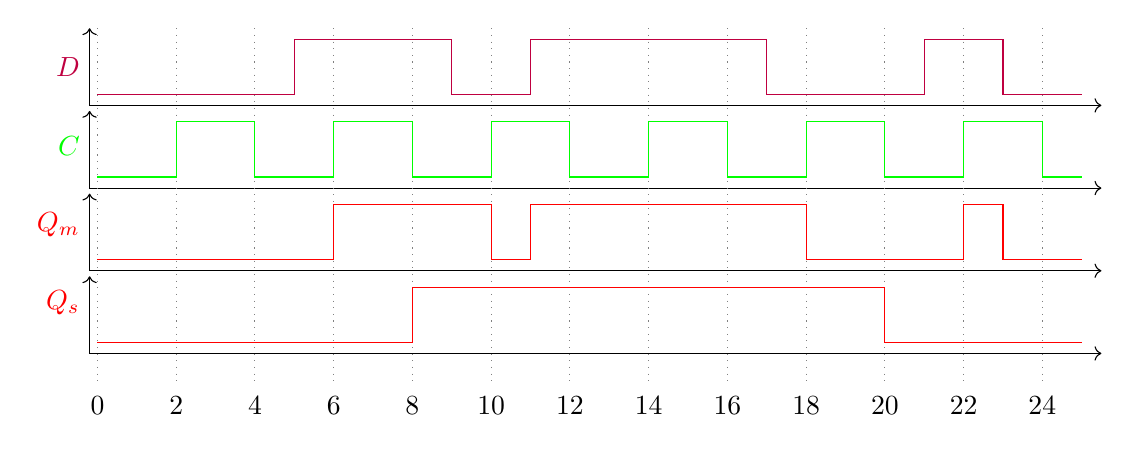
\begin{tikzpicture}[xscale=0.5, yscale=0.7]
        \draw[<->] (-0.2, 1.2) -- (-0.2, -0.2) -- (25.5, -0.2); 
        \draw[<->, yshift=-1.5cm] (-0.2, 1.2) -- (-0.2, -0.2) -- (25.5, -0.2); 
        \draw[<->, yshift=-3cm] (-0.2, 1.2) -- (-0.2, -0.2) -- (25.5, -0.2); 
        \draw[<->, yshift=-4.5cm] (-0.2, 1.2) -- (-0.2, -0.2) -- (25.5, -0.2); 
        
        % Time labels and dotted lines for bottom graph only
        \foreach \x in {0, 2, 4, 6, 8, 10, 12, 14, 16, 18, 20, 22, 24} {
          \draw[dotted, gray] (\x, 1.2) -- (\x, -5.3);
          \node[below] at (\x, -5.3) {\x};
        }
        
        \node[purple, left] at (-0.2, 0.5) {$D$}; 
        \node[green, left, yshift=-1cm] at (-0.2, 0.5) {$C$}; 
        \node[red, left, yshift=-2cm] at (-0.2, 0.5) {$Q_m$}; 
        \node[red, left, yshift=-3cm] at (-0.2, 0.5) {$Q_s$}; 
        
        \draw[purple] (0, 0) -- 
          (5, 0) -- (5, 1) -- (9, 1) -- (9, 0) -- 
          (11, 0) -- (11, 1) -- (17, 1) -- (17, 0) -- 
          (21, 0) -- (21, 1) -- (23, 1) -- (23, 0) -- 
          (25, 0);
        \draw[green, yshift=-1.5cm] (0, 0) -- 
          (2, 0) -- (2, 1) -- (4, 1) -- (4, 0) -- 
          (6, 0) -- (6, 1) -- (8, 1) -- (8, 0) -- 
          (10, 0) -- (10, 1) -- (12, 1) -- (12, 0) -- 
          (14, 0) -- (14, 1) -- (16, 1) -- (16, 0) -- 
          (18, 0) -- (18, 1) -- (20, 1) -- (20, 0) -- 
          (22, 0) -- (22, 1) -- (24, 1) -- (24, 0) -- 
          (25, 0); 
        \draw[red, yshift=-3cm] (0, 0) -- 
          (6, 0) -- (6, 1) -- (10, 1) -- (10, 0) -- 
          (11, 0) -- (11, 1) -- (18, 1) -- (18, 0) -- 
          (22, 0) -- (22, 1) -- (23, 1) -- (23, 0) -- 
          (25, 0); 
        \draw[red, yshift=-4.5cm] (0, 0) -- 
          (8, 0) -- (8, 1) -- (20, 1) -- (20, 0) -- 
          (25, 0);
      \end{tikzpicture}
      \caption{}
    \end{figure}
  \end{example}
  
  We revisit the problem of invalid states for SR latches, which lead to race conditions (both 1s for active high and both 0s for active low). We introduce the JK latch, which is not a flip flop yet. Note that you put a pulse through $K$ to reset $Q = 0$, and a pulse through $J$ to set $Q = 1$.

  \begin{figure}[H]
    \centering
    \begin{subfigure}[b]{0.48\textwidth}
      \centering
      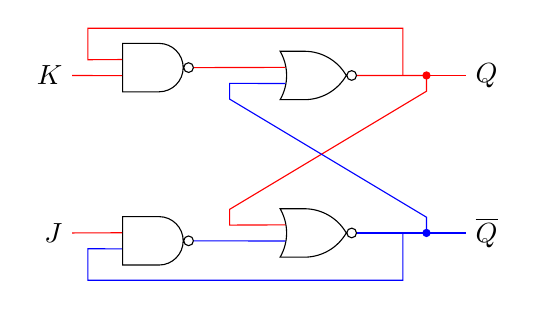
\begin{tikzpicture}[circuit logic US]
        \node[nand gate] (nand1) at (-2, 1.1) {};
        \node[nand gate] (nand2) at (-2, -1.1) {};
        \node[nor gate] (nor1) at (0, 1) {}; 
        \node[nor gate] (nor2) at (0, -1) {}; 

        \draw[red] (-3, 1.0) -- (nand1.input 2);
        \draw[red] (-3, -1.0) -- (nand2.input 1);
        \node[left] at (-3,1.0) {$K$};
        \node[left] at (-3,-1.0) {$J$};
        \node[right] at (2, 1) {$Q$};
        \node[right] at (2, -1) {$\overline{Q}$};

        \draw[red] (nand1.input 1) -- (-2.8, 1.2) -- (-2.8, 1.6) -- (1.2, 1.6) -- (1.2, 1); 
        \draw[blue] (nand2.input 2) -- (-2.8, -1.2) -- (-2.8, -1.6) -- (1.2, -1.6) -- (1.2, -1); 

        \draw[red] (nand1.output) -- (nor1.input 1);
        \draw[blue] (nand2.output) -- (nor2.input 2);
        \draw[red] (nor1.output) -- (2, 1); 
        \draw[blue] (nor2.output) -- (2, -1); 

        \draw[red] (nor1.output) -- (1.5, 1) -- (1.5, 0.8) -- (-1, -0.7) -- (-1, -0.9) -- (nor2.input 1);
        \draw[blue] (nor2.output) -- (1.5, -1) -- (1.5, -0.8) -- (-1, 0.7) -- (-1, 0.9) -- (nor1.input 2);
        \fill[red] (1.5,1) circle (1.5pt);
        \fill[blue] (1.5,-1) circle (1.5pt);
      \end{tikzpicture} 
      \caption{}
    \end{subfigure}
    \hfill 
    \begin{subfigure}[b]{0.48\textwidth}
      \centering
      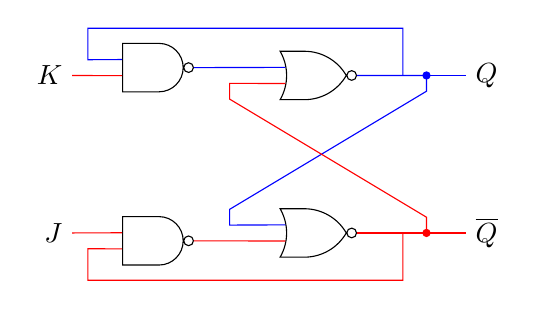
\begin{tikzpicture}[circuit logic US]
        \node[nand gate] (nand1) at (-2, 1.1) {};
        \node[nand gate] (nand2) at (-2, -1.1) {};
        \node[nor gate] (nor1) at (0, 1) {}; 
        \node[nor gate] (nor2) at (0, -1) {}; 

        \draw[red] (-3, 1.0) -- (nand1.input 2);
        \draw[red] (-3, -1.0) -- (nand2.input 1);
        \node[left] at (-3,1.0) {$K$};
        \node[left] at (-3,-1.0) {$J$};
        \node[right] at (2, 1) {$Q$};
        \node[right] at (2, -1) {$\overline{Q}$};

        \draw[blue] (nand1.input 1) -- (-2.8, 1.2) -- (-2.8, 1.6) -- (1.2, 1.6) -- (1.2, 1); 
        \draw[red] (nand2.input 2) -- (-2.8, -1.2) -- (-2.8, -1.6) -- (1.2, -1.6) -- (1.2, -1); 

        \draw[blue] (nand1.output) -- (nor1.input 1);
        \draw[red] (nand2.output) -- (nor2.input 2);
        \draw[blue] (nor1.output) -- (2, 1); 
        \draw[red] (nor2.output) -- (2, -1); 

        \draw[blue] (nor1.output) -- (1.5, 1) -- (1.5, 0.8) -- (-1, -0.7) -- (-1, -0.9) -- (nor2.input 1);
        \draw[red] (nor2.output) -- (1.5, -1) -- (1.5, -0.8) -- (-1, 0.7) -- (-1, 0.9) -- (nor1.input 2);
        \fill[blue] (1.5,1) circle (1.5pt);
        \fill[red] (1.5,-1) circle (1.5pt);
      \end{tikzpicture} 
      \caption{}
    \end{subfigure}
    \caption{JK active high latch. When you set $J = K = 1$, the latch oscillates between $Q = 0$ and $Q = 1$ very fast, but this eliminates the possibility where $Q$ is both $1$ or both $0$.}
  \end{figure}

  Note that we can do the same with an active low JK latch, which will be functionally identical to the active high one. Now we are a step closer to the JK flip flop. By adding a gate/enabler and synching it with the clock, we can get the \textit{level triggered JK flip flop}. 

  \begin{figure}[H]
    \centering 
    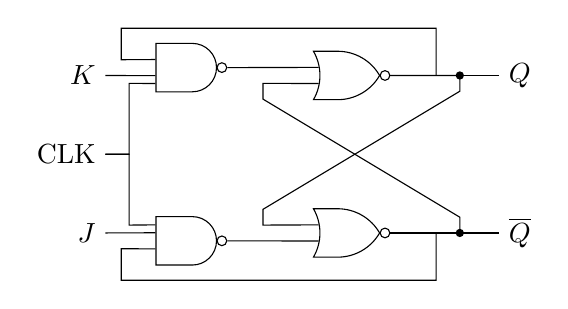
\begin{tikzpicture}[circuit logic US]
      \node[nand gate] (nand1) at (-2, 1.1) {};
      \node[nand gate] (nand2) at (-2, -1.1) {};
      \node[nor gate] (nor1) at (0, 1) {}; 
      \node[nor gate] (nor2) at (0, -1) {}; 
      \draw (-3, 0) -- (-2.7, 0) -- (-2.7, 0.9) -- ([yshift=-0.1cm]nand1.input 2); 
      \draw (-3, 0) -- (-2.7, 0) -- (-2.7, -0.9) -- ([yshift=0.1cm]nand2.input 1); 

      \draw[] (-3, 1.0) -- (nand1.input 2);
      \draw[] (-3, -1.0) -- (nand2.input 1);
      \node[left] at (-3,1.0) {$K$};
      \node[left] at (-3,-1.0) {$J$};
      \node[left] at (-3,0) {CLK};
      \node[right] at (2, 1) {$Q$};
      \node[right] at (2, -1) {$\overline{Q}$};

      \draw[] (nand1.input 1) -- (-2.8, 1.2) -- (-2.8, 1.6) -- (1.2, 1.6) -- (1.2, 1); 
      \draw[] (nand2.input 2) -- (-2.8, -1.2) -- (-2.8, -1.6) -- (1.2, -1.6) -- (1.2, -1); 

      \draw[] (nand1.output) -- (nor1.input 1);
      \draw[] (nand2.output) -- (nor2.input 2);
      \draw[] (nor1.output) -- (2, 1); 
      \draw[] (nor2.output) -- (2, -1); 

      \draw[] (nor1.output) -- (1.5, 1) -- (1.5, 0.8) -- (-1, -0.7) -- (-1, -0.9) -- (nor2.input 1);
      \draw[] (nor2.output) -- (1.5, -1) -- (1.5, -0.8) -- (-1, 0.7) -- (-1, 0.9) -- (nor1.input 2);
      \fill[] (1.5,1) circle (1.5pt);
      \fill[] (1.5,-1) circle (1.5pt);
    \end{tikzpicture} 
    \caption{Level Triggered JK Flip Flop. } 
  \end{figure}

  \begin{example}[Waveforms of Level Triggered JK Flip Flop]
    Let's go through the timing diagram. 
    \begin{enumerate}
      \item $t = 1$. When $K = 1$, there is no change in $Q$ since the clock is low. The flip flop is disabled. 
      \item $t = 2$. The clock is high and the reset signal goes through the AND gate, and $Q = 0$. 
      \item $t = 10$. $J$ becomes high and the clock is high, enabling the latch again, and consequently $Q$ is high again. 
      \item $t = 18, 22, 26$. When $C, J, K$ are all high, then the circuit begins to oscillate uncontrollably.  
    \end{enumerate}

    \begin{figure}[H]
      \centering 
      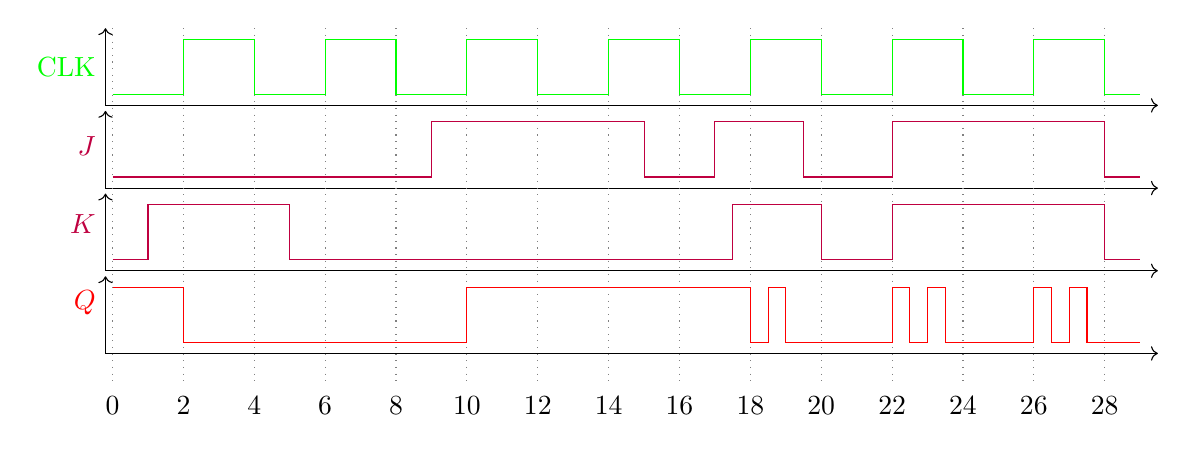
\begin{tikzpicture}[xscale=0.45, yscale=0.7]
        \draw[<->] (-0.2, 1.2) -- (-0.2, -0.2) -- (29.5, -0.2); 
        \draw[<->, yshift=-1.5cm] (-0.2, 1.2) -- (-0.2, -0.2) -- (29.5, -0.2); 
        \draw[<->, yshift=-3cm] (-0.2, 1.2) -- (-0.2, -0.2) -- (29.5, -0.2); 
        \draw[<->, yshift=-4.5cm] (-0.2, 1.2) -- (-0.2, -0.2) -- (29.5, -0.2); 
        
        % Time labels and dotted lines for bottom graph only
        \foreach \x in {0, 2, 4, 6, 8, 10, 12, 14, 16, 18, 20, 22, 24, 26, 28} {
          \draw[dotted, gray] (\x, 1.2) -- (\x, -5.3);
          \node[below] at (\x, -5.3) {\x};
        }
        
        \node[green, left] at (-0.2, 0.5) {CLK}; 
        \node[purple, left, yshift=-1cm] at (-0.2, 0.5) {$J$}; 
        \node[purple, left, yshift=-2cm] at (-0.2, 0.5) {$K$}; 
        \node[red, left, yshift=-3cm] at (-0.2, 0.5) {$Q$}; 
        
        \draw[green] (0, 0) -- 
          (2, 0) -- (2, 1) -- (4, 1) -- (4, 0) -- 
          (6, 0) -- (6, 1) -- (8, 1) -- (8, 0) -- 
          (10, 0) -- (10, 1) -- (12, 1) -- (12, 0) -- 
          (14, 0) -- (14, 1) -- (16, 1) -- (16, 0) -- 
          (18, 0) -- (18, 1) -- (20, 1) -- (20, 0) -- 
          (22, 0) -- (22, 1) -- (24, 1) -- (24, 0) -- 
          (26, 0) -- (26, 1) -- (28, 1) -- (28, 0) -- 
          (29, 0); 
        \draw[purple, yshift=-1.5cm] (0, 0) -- 
          (9, 0) -- (9, 1) -- (15, 1) -- (15, 0) -- 
          (17, 0) -- (17, 1) -- (19.5, 1) -- (19.5, 0) -- 
          (22, 0) -- (22, 1) -- (28, 1) -- (28, 0) -- 
          (29, 0); 
        \draw[purple, yshift=-3cm] (0, 0) -- 
          (1, 0) -- (1, 1) -- (5, 1) -- (5, 0) -- 
          (17.5, 0) -- (17.5, 1) -- (20, 1) -- (20, 0) -- 
          (22, 0) -- (22, 1) -- (28, 1) -- (28, 0) -- 
          (29, 0); 
        \draw[red, yshift=-4.5cm] 
          (0, 1) -- (2, 1) -- (2, 0) -- 
          (10, 0) -- (10, 1) -- (18, 1) -- (18, 0) --
          (18.5, 0) -- (18.5, 1) -- (19, 1) -- (19, 0) --
          (22, 0) -- (22, 1) -- (22.5, 1) -- (22.5, 0) -- 
          (23, 0) -- (23, 1) -- (23.5, 1) -- (23.5, 0) -- 
          (26, 0) -- (26, 1) -- (26.5, 1) -- (26.5, 0) -- 
          (27, 0) -- (27, 1) -- (27.5, 1) -- (27.5, 0) -- 
          (29, 0);
      \end{tikzpicture}
      \caption{}
    \end{figure}
  \end{example}

  To take advantage of this oscillation, we need a flip flop that will only react the inputs while the clock singal is changing from low to high, i.e. on the rising edge. 

  \begin{definition}[Edge Triggered JK Flip Flop]
    To fix the weird oscillation issues, we can use the edge detection device to get the \textbf{edge triggered JK flip-flop}. 

    \begin{figure}[H]
      \centering 
      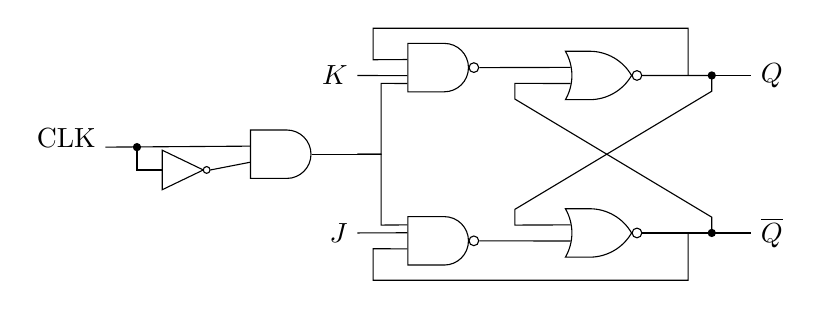
\begin{tikzpicture}[circuit logic US]
        \node[and gate] (and) at (-4, 0) {};
        \node[not gate, scale=0.7] (not) at (-5.3, -0.2) {};
        \draw (-6.2, 0.09) -- (and.input 1);
        \draw (-5.8, 0.09) -- (-5.8, -0.2) -- (not.input);
        \fill (-5.8, 0.09) circle (1.5pt); 
        \node[left] at (-6.2, 0.2) {CLK}; 
        \draw(and.output) -- (-2.7, 0);
        \draw(not.output) -- (and.input 2); 

        \node[nand gate] (nand1) at (-2, 1.1) {};
        \node[nand gate] (nand2) at (-2, -1.1) {};
        \node[nor gate] (nor1) at (0, 1) {}; 
        \node[nor gate] (nor2) at (0, -1) {}; 
        \draw (-3, 0) -- (-2.7, 0) -- (-2.7, 0.9) -- ([yshift=-0.1cm]nand1.input 2); 
        \draw (-3, 0) -- (-2.7, 0) -- (-2.7, -0.9) -- ([yshift=0.1cm]nand2.input 1); 

        \draw[] (-3, 1.0) -- (nand1.input 2);
        \draw[] (-3, -1.0) -- (nand2.input 1);
        \node[left] at (-3,1.0) {$K$};
        \node[left] at (-3,-1.0) {$J$};
        \node[right] at (2, 1) {$Q$};
        \node[right] at (2, -1) {$\overline{Q}$};

        \draw[] (nand1.input 1) -- (-2.8, 1.2) -- (-2.8, 1.6) -- (1.2, 1.6) -- (1.2, 1); 
        \draw[] (nand2.input 2) -- (-2.8, -1.2) -- (-2.8, -1.6) -- (1.2, -1.6) -- (1.2, -1); 

        \draw[] (nand1.output) -- (nor1.input 1);
        \draw[] (nand2.output) -- (nor2.input 2);
        \draw[] (nor1.output) -- (2, 1); 
        \draw[] (nor2.output) -- (2, -1); 

        \draw[] (nor1.output) -- (1.5, 1) -- (1.5, 0.8) -- (-1, -0.7) -- (-1, -0.9) -- (nor2.input 1);
        \draw[] (nor2.output) -- (1.5, -1) -- (1.5, -0.8) -- (-1, 0.7) -- (-1, 0.9) -- (nor1.input 2);
        \fill[] (1.5,1) circle (1.5pt);
        \fill[] (1.5,-1) circle (1.5pt);
      \end{tikzpicture} 
      \caption{Edge Triggered JK Flip Flop. } 
    \end{figure}
  \end{definition}

  It is also called the \textit{universal programmable flip flop} since you can make other types of flip flops from JK flip flops. 

  \begin{example}[Waveforms of Edge Triggered JK Flip Flop]
    With the edge detector, only the rising edge of each clock pulse has any effect. Notice that when $J$ and $K$ are both high, a clock pulse will cause the flip flop to toggle from one state to the other (at times $t = 18, 22, 26$).  

    \begin{figure}[H]
      \centering 
      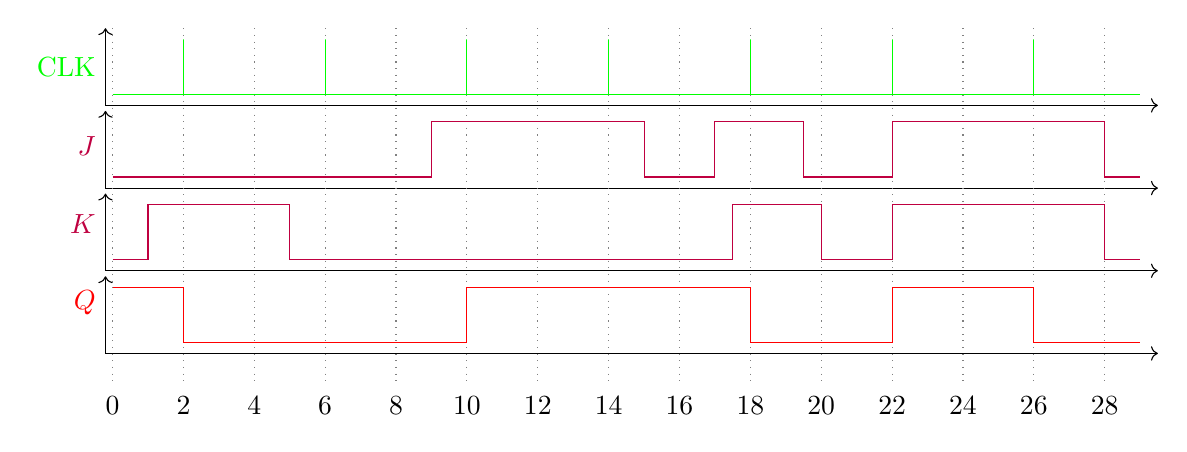
\begin{tikzpicture}[xscale=0.45, yscale=0.7]
        \draw[<->] (-0.2, 1.2) -- (-0.2, -0.2) -- (29.5, -0.2); 
        \draw[<->, yshift=-1.5cm] (-0.2, 1.2) -- (-0.2, -0.2) -- (29.5, -0.2); 
        \draw[<->, yshift=-3cm] (-0.2, 1.2) -- (-0.2, -0.2) -- (29.5, -0.2); 
        \draw[<->, yshift=-4.5cm] (-0.2, 1.2) -- (-0.2, -0.2) -- (29.5, -0.2); 
        
        % Time labels and dotted lines for bottom graph only
        \foreach \x in {0, 2, 4, 6, 8, 10, 12, 14, 16, 18, 20, 22, 24, 26, 28} {
          \draw[dotted, gray] (\x, 1.2) -- (\x, -5.3);
          \node[below] at (\x, -5.3) {\x};
        }
        
        \node[green, left] at (-0.2, 0.5) {CLK}; 
        \node[purple, left, yshift=-1cm] at (-0.2, 0.5) {$J$}; 
        \node[purple, left, yshift=-2cm] at (-0.2, 0.5) {$K$}; 
        \node[red, left, yshift=-3cm] at (-0.2, 0.5) {$Q$}; 
        
        \draw[green] (0, 0) -- 
          (2, 0) -- (2, 1) -- (2, 0) -- (4, 0) -- 
          (6, 0) -- (6, 1) -- (6, 0) -- (8, 0) -- 
          (10, 0) -- (10, 1) -- (10, 0) -- (12, 0) -- 
          (14, 0) -- (14, 1) -- (14, 0) -- (16, 0) -- 
          (18, 0) -- (18, 1) -- (18, 0) -- (20, 0) -- 
          (22, 0) -- (22, 1) -- (22, 0) -- (24, 0) -- 
          (26, 0) -- (26, 1) -- (26, 0) -- (28, 0) -- 
          (29, 0); 
        \draw[purple, yshift=-1.5cm] (0, 0) -- 
          (9, 0) -- (9, 1) -- (15, 1) -- (15, 0) -- 
          (17, 0) -- (17, 1) -- (19.5, 1) -- (19.5, 0) -- 
          (22, 0) -- (22, 1) -- (28, 1) -- (28, 0) -- 
          (29, 0); 
        \draw[purple, yshift=-3cm] (0, 0) -- 
          (1, 0) -- (1, 1) -- (5, 1) -- (5, 0) -- 
          (17.5, 0) -- (17.5, 1) -- (20, 1) -- (20, 0) -- 
          (22, 0) -- (22, 1) -- (28, 1) -- (28, 0) -- 
          (29, 0); 
        \draw[red, yshift=-4.5cm] 
          (0, 1) -- (2, 1) -- (2, 0) -- 
          (10, 0) -- (10, 1) -- (18, 1) -- (18, 0) --
          (22, 0) -- (22, 1) -- (26, 1) -- (26, 0) -- 
          (29, 0);
      \end{tikzpicture}
      \caption{}
    \end{figure}
  \end{example}

  Another simple modification of the JK flip flop gives us another type of flip flop. B simply connecting together $J$ and $K$ to make one input, we now have a device that will toggle from one state to the other when the input is high at the rising edge of the clock. 

  \begin{definition}[T-Type Flip Flip]
    The \textbf{T-Type flip flop}. 

    \begin{figure}[H]
      \centering 
      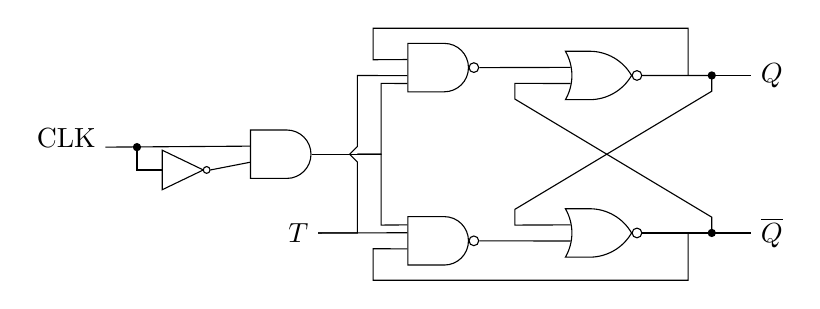
\begin{tikzpicture}[circuit logic US]
        \node[and gate] (and) at (-4, 0) {};
        \node[not gate, scale=0.7] (not) at (-5.3, -0.2) {};
        \draw (-6.2, 0.09) -- (and.input 1);
        \draw (-5.8, 0.09) -- (-5.8, -0.2) -- (not.input);
        \fill (-5.8, 0.09) circle (1.5pt); 
        \node[left] at (-6.2, 0.2) {CLK}; 
        \draw(and.output) -- (-2.7, 0);
        \draw(not.output) -- (and.input 2); 

        \node[nand gate] (nand1) at (-2, 1.1) {};
        \node[nand gate] (nand2) at (-2, -1.1) {};
        \node[nor gate] (nor1) at (0, 1) {}; 
        \node[nor gate] (nor2) at (0, -1) {}; 
        \draw (-3, 0) -- (-2.7, 0) -- (-2.7, 0.9) -- ([yshift=-0.1cm]nand1.input 2); 
        \draw (-3, 0) -- (-2.7, 0) -- (-2.7, -0.9) -- ([yshift=0.1cm]nand2.input 1); 

        \draw[] (-3.5, -1.0) -- (-3, -1.0) -- (-3, -0.1) -- (-3.1, 0) -- (-3, 0.1) -- (-3, 1.0) -- (nand1.input 2); 
        \draw[] (-3.5, -1.0) -- (nand2.input 1);
        \node[left] at (-3.5,-1.0) {$T$};
        \node[right] at (2, 1) {$Q$};
        \node[right] at (2, -1) {$\overline{Q}$};

        \draw[] (nand1.input 1) -- (-2.8, 1.2) -- (-2.8, 1.6) -- (1.2, 1.6) -- (1.2, 1); 
        \draw[] (nand2.input 2) -- (-2.8, -1.2) -- (-2.8, -1.6) -- (1.2, -1.6) -- (1.2, -1); 

        \draw[] (nand1.output) -- (nor1.input 1);
        \draw[] (nand2.output) -- (nor2.input 2);
        \draw[] (nor1.output) -- (2, 1); 
        \draw[] (nor2.output) -- (2, -1); 

        \draw[] (nor1.output) -- (1.5, 1) -- (1.5, 0.8) -- (-1, -0.7) -- (-1, -0.9) -- (nor2.input 1);
        \draw[] (nor2.output) -- (1.5, -1) -- (1.5, -0.8) -- (-1, 0.7) -- (-1, 0.9) -- (nor1.input 2);
        \fill[] (1.5,1) circle (1.5pt);
        \fill[] (1.5,-1) circle (1.5pt);
      \end{tikzpicture} 
      \caption{Edge triggered JK flip flop. } 
    \end{figure}
  \end{definition}

\subsection{Registers}

  To understand anything that the CPU does, we must understand assembly language. In here, everything is done within registers, and we can see how the CPU fetches, decodes, and executes instructions. So what exactly are these registers? 

  \begin{definition}[Register]
    A register is a small, fast storage location within the CPU. It is used to store data that is being used immediately, and is the only place where the CPU can perform operations, which is why it must move data from memory to registers before it can perform operations on it. Everything in a register is in binary, at most 8 bytes, or 64 bits. 

    There are very specific types of registers that you should know. All of these registers are implemented for all assembly languages and are integral to the workflow of the CPU.  
    \begin{enumerate}
      \item \textbf{parameter registers} which store the parameters of a function.
      \item \textbf{Return registers} which store return values of functions. 
      \item \textbf{stack pointers} which point to the top of the stack (at the top of the current stack frame). 
      \item \textbf{frame pointers} which point to the base of the current stack frame.
      \item \textbf{instruction pointers} which point to the next instruction to be executed.
    \end{enumerate}
  \end{definition}

  \begin{definition}[32 and 64 Bit Machines]
    There are two types of machines that tend to format these boxes very differently: 32-bit and 64-bit machines. 
    \begin{enumerate}
      \item 32 bit machines store addresses in 32 bits, so they can have $2^{32}$ addresses, which is about 4 GB of memory. 
      \item 64 bit machines store addresses in 64 bits, so they can have $2^{64}$ addresses, which is about 16 EB of memory. This does not mean that the actual RAM is 16 EB, but it means that the machine can \textit{handle} that much memory. 
      \begin{lstlisting} 
        ...
        0x00007FFF7FBFF860 --> 0b000000000000000000000000011111111111
                               111101111111101111111111100001100000
        0x00007FFF7FBFF861 --> 0b000000000000000000000000011111111111
                               111101111111101111111111100001100001
        0x00007FFF7FBFF862 --> 0b000000000000000000000000011111111111
                               111101111111101111111111100001100010
        0x00007FFF7FBFF863 --> 0b000000000000000000000000011111111111
                               111101111111101111111111100001100011
        0x00007FFF7FBFF864 --> 0b000000000000000000000000011111111111
                               111101111111101111111111100001100100
        ...
      \end{lstlisting}
    \end{enumerate}
    The numbers typically mean the size of the type that the machine works best with, so all memory addresses will be 32 or 64 bits wide. Most machines are 64-bits, and so everything in this notes will assume that we are working with a 64 bit machine. As we will later see, this is why pointers are 8 bytes long, i.e. 64 bits. This is because the memory addresses are 64 bits long, though all of them are not used. 
  \end{definition}

\subsection{Memory Banks}

  \begin{definition}[Memory]
    The \textbf{memory} is where the computer stores data and instructions, which can be though of as a giant array of memory addresses, with each containing a byte. This data consists of graphical things or even instructions to manipulate other data. It can be visualized  as a long array of boxes that each have an \textbf{address} (where it is located) and \textbf{contents} (what is stored in it).

    Memory simply works as a bunch of bits in your computer with each bit having some memory address, which is also a bit. For example, the memory address \texttt{0b0010} (2) may have the bit value of \texttt{0b1} (1) stored in it. 

    \begin{figure}[H]
      \centering 
      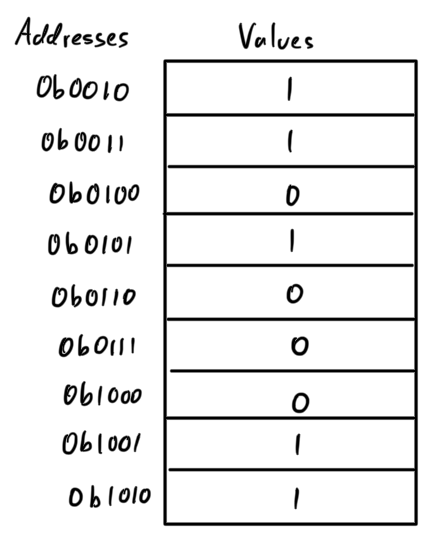
\includegraphics[scale=0.4]{img/memory_visual_bit.png}
      \caption{Visualization of memory as a long array of boxes of bits. }
      \label{fig:memory_visual_bit}
    \end{figure}

    However, computers do not need this fine grained level of control on the memory, and they really work at the Byte level rather than the bit level. Therefore, we can visualize the memory as a long array of boxes indexed by \textit{Bytes}, with each value being a byte as well. In short, the memory is \textbf{byte-addressable}. In certain arthitectures, some systems are \textbf{word-addressable}, meaning that the memory is addressed by words, which are 4 bytes.\footnote{Note that in here the size of a word is 2 bytes rather than 4 as stated above. This is just how it is defined in some \texttt{x86} architectures.}

    \begin{figure}[H]
      \centering 
      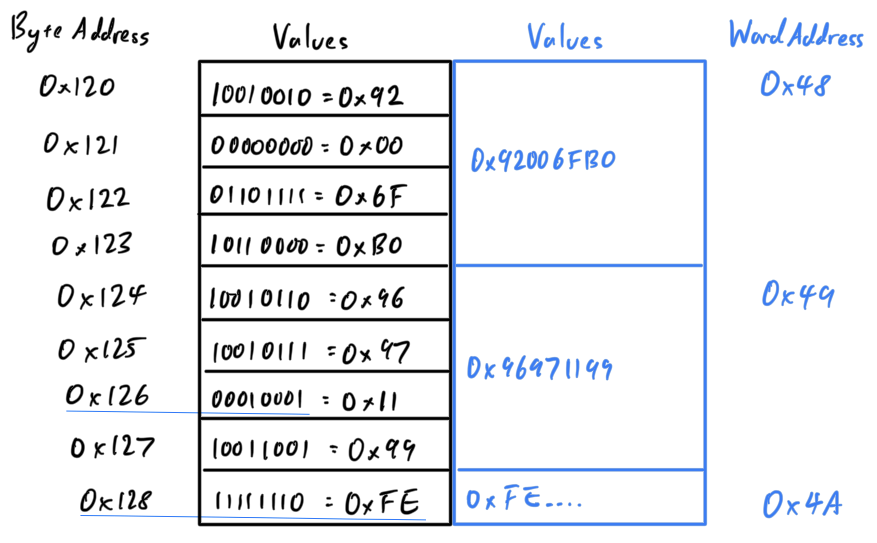
\includegraphics[scale=0.4]{img/memory_visual_byte.png}
      \caption{Visualization of memory as a long array of boxes of bytes. Every address is a byte and its corresponding value at that address is also a byte, though we represent it as a 2-digit hex. } 
      \label{fig:memory_visual_byte}
    \end{figure}
  \end{definition}

  It is intuitive to think that given some multi-byte object like an \texttt{int} (4 bytes), the beginning of the int would be the lowest address and the end of the int would be the highest address, like how consecutive integers are stored in an array. However, this is not always the case (almost always not the case since most computers are little-endian).  

  \begin{definition}[Endian Architecture]
    Depending on the machine architecture, computers may store these types slightly differently in their \textit{byte} order. Say that we have an integer of value \texttt{0xA1B2C3D4} (4 bytes). Then, 
    \begin{enumerate} 
      \item A \textbf{big-endian architecture} (e.g. SPARC, z/Architecture) will store it so that the least significant byte has the highest address.
      \item A \textbf{little-endian architecture} (e.g. x86, x86-64, RISC-V) will store it so that the least significant byte has the lowest address. 
      \item A \textbf{bi-endian architecture} (e.g. ARM, PowerPC) can specify the endianness as big or little. 
    \end{enumerate}

    \begin{figure}[H]
      \centering 
      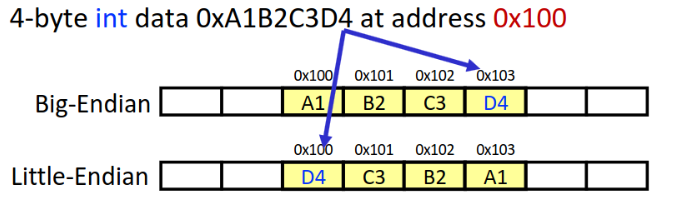
\includegraphics[scale=0.4]{img/endianness.png}
      \caption{The big vs little endian architectures. } 
      \label{fig:endianness}
    \end{figure}
  \end{definition}

  We can simply print out the hex values of primitive types to see how they are stored in memory, but it does not provide the level of details that we want on which bytes are stored where. At this point, we must use certain \textbf{debuggers} to directly look at the memory. For x86 architectures, we can use \texttt{gdb} and for ARM architectures, we can use \texttt{lldb}. At this point, we need to understand assembly to look through debuggers, so we will provide the example here. 

  \begin{example}[Endianness of C Int in x86-64]
    To do. 
  \end{example}

  \begin{example}[Endianness of C Int in ARM64]
    To do. 
  \end{example}

\subsection{Counter Chips}

\section{Binary Encodings} 
  
  We have motivated the need for \textit{binary} encodings through the construction of the transistor. In retrospect, we can therefore see why we want to develop a theory around \hyperref[th-binary_motivation]{binary alphabets} in $\{0, 1\}^\ast$. Now that we know how to work with them, the remaining task of encoding elements of an arbitrary set $S \to \{0, 1\}^\ast = \sqcup_n \{0, 1\}^n$ is mathematically trivial. 

  \begin{definition}[Representation Scheme]
    A \textbf{representation scheme} is an encoding of an object $s$ to a unique binary string $E(s) \in \{0,1\}^\ast$. It is an injective function 
    \begin{equation}
      E: X \longrightarrow \{0,1\}^\ast
    \end{equation}
  \end{definition}

  Therefore, when we say that a program $P$ takes $x$ as an input, we really mean that $P$ takes as input the \textit{representation of $x$} as a binary string.  

  Since $\{0, 1\}^\ast$ is \hyperref[set-def:countable]{countable}, there always exists an injective map $f: S \to \{0, 1\}^\ast$ as long as $S$ is at most countable. But in practicality, we would like to find a good encoding that is easy to work with. Throughout this chapter, we will consider different sets $S$ and introduce the standard encodings for each set. 

  In order to get into memory, it is helpful to know the theory behind how primitive types are stored in memory.  

  \begin{definition}[Collections of Bits]
    There are many words that are used to talk about values of different data types: 
    \begin{enumerate}
      \item A \textbf{bit} (b) is either $0$ or $1$. 
      \item A \textbf{Hex} (x) is a collection of 4 bits, with a total of $2^4 = 16$ possible values, and this is used since it is easy to read for humans. 
      \item A \textbf{Byte} (B) is a collection of 8 bits or 2 hex, with a total of $2^8 = 256$ possible values, and most computers will work with Bytes as the smallest unit of memory. 
    \end{enumerate}
  \end{definition}

\subsection{Naturals/Unsigned and Integers/Signed}

  \begin{definition}[Representation of the Naturals]
    A representation for natural numbers (note that in this context, $0 \in \mathbb{N}$) is the (non-surjective) regular binary representation denoted
    \begin{equation}
      NtS: \mathbb{N} \longrightarrow \{0,1\}^\ast \;\;\;\; (NtS= \text{ "Naturals to Strings"})
    \end{equation}
    recursively defined as 
    \[NtS(n) = \begin{cases}
    0 & n = 0 \\
    1 & n = 1 \\
    NtS(\left \lceil{n/2}\right \rceil parity(n) & n > 1 
    \end{cases}\]
    where given strings $x, y \in \{0,1\}^\ast$, $xy$ denotes the concatenation of $x$ and $y$, and $parity: \mathbb{N} \longrightarrow \{0,1\}^\ast$ is defined 
    \[parity(n) = \begin{cases}
    0 & n $\text{ is even}$ \\
    1 & n $\text{ is odd}$
    \end{cases}\]
    Since $NtS$ in injective, its inverse $StN: \mathrm{Im}{NtS} \subset \{0,1\}^\ast \longrightarrow \mathbb{N}$ is well-defined. 
  \end{definition}

  \begin{definition}[Representation of the Integers]
    To construct a representation scheme for $\mathbb{Z}$, we can just add one more binary digit to represent the sign of the number. The binary representation $ZtS: \mathbb{Z} \longrightarrow \{0, 1\}^\ast$ is defined
    \[ZtS(m) = \begin{cases}
    0\, NtS(m) & m \geq 0 \\
    1 \, NtS(-m) & m < 0
    \end{cases}\]
    where $NtS$ is defined as before. Again this function must be injective but need not be surjective. 
  \end{definition}

  The most primitive things that we can store are integers. Let us talk about how we represent some of the simplest primitive types in C: unsigned short, unsigned int, unsigned long, unsigned long long.

  \begin{definition}[Unsigned Integer Types in C]
    In C, there are several integer types. We use this hierarchical method to give flexibility to the programmer on the size of the integer and whether it is signed or not. 
    \begin{enumerate} 
      \item An \textbf{unsigned short} is 2 bytes long and can be represented as a 4-digit hex or 16 bits, with values in $[0:65,535]$. Therefore, say that we have 
      \item An \textbf{unsigned int} is 4 bytes long and can be represented as an 8-digit hex or 32 bits, with values in $[0:4,294,967,295]$. 
      \item An \textbf{unsigned long} is 8 bytes and can be represented as an 16-digit hex or 64 bits, but they are only guaranteed to be stored in 32 bits in other systems. 
      \item An \textbf{unsigned long long} is 8 bytes and can be represented as an 16-digit hex or 64 bits, and they are guaranteed to be stored in 64 bits in other systems. 
    \end{enumerate} 
  \end{definition}

  \begin{theorem}[Bit Representation of Unsigned Integers in C]
    To encode a signed integer in bits, we simply take the binary expansion of it. 
    \begin{figure}[H]
      \centering 
      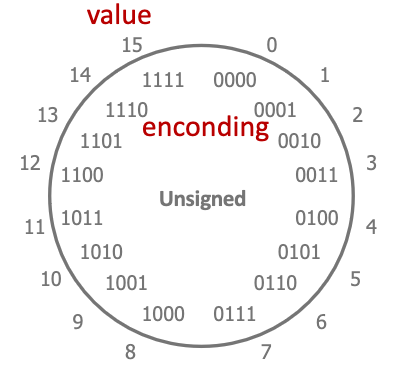
\includegraphics[scale=0.4]{img/unsigned_encoding.png}
      \caption{Unsigned encoding of 4-bit integers in C. } 
      \label{fig:unsigned_encoding}
    \end{figure}
  \end{theorem}

  \begin{example}[Bit Representation of Unsigned Integers in C]
    We can see for ourselves how these numbers are represented in bits. Printing the values out in binary requires to make new functions, but we can easily convert from hex to binary. 

    \noindent\begin{minipage}{.5\textwidth}
    \begin{lstlisting}[]{Code}
      int main() { 

        unsigned short x = 13; 
        unsigned int y = 256;

        printf("%x\n", x);
        printf("%x\n", y);

        return 0; 
      }
    \end{lstlisting}
    \end{minipage}
    \hfill
    \begin{minipage}{.49\textwidth}
    \begin{lstlisting}[]{Output}
      d
      100 
      .
      .
      .
      .
      .
      .
      .
      .
    \end{lstlisting}
    \end{minipage}
  \end{example}

  So far, the process of converting unsigned numbers to bits seemed simple. Now let's introduce signed integers. 

  \begin{definition}[Signed Integer Types in C]
    In C, there are several signed integer types. We use this hierarchical method to give flexibility to the programmer on the size of the integer and whether it is signed or not. 
    \begin{enumerate} 
      \item A \textbf{signed short} is 2 bytes long and can be represented as a 4-digit hex or 16 bits, with values in $[-32,768: 32,767]$. 
      \item A \textbf{signed int} is 4 bytes long and can be represented as an 8-digit hex or 32 bits, with values in $[-2,147,483,648: 2,147,483,647]$. 
      \item A \textbf{signed long} is 8 bytes and can be represented as an 16-digit hex or 64 bits, but they are only guaranteed to be stored in 32 bits in other systems. 
      \item A \textbf{signed long long} is 8 bytes and can be represented as an 16-digit hex or 64 bits, and they are guaranteed to be stored in 64 bits in other systems. 
    \end{enumerate}
  \end{definition}

  To store signed integers, it is intuitive to simply take the first (left-most) bit and have that be the sign. Therefore, we lose one significant figure but gain information about the sign. However, this has some problems: first, there are two representations of zeros: $-0$ and $+0$. Second, the continuity from $-1$ to $0$ is not natural. It is best explained through an example, which doesn't lose much insight into the general case. 

  \begin{example}[Problems with the Signed Magnitude]
    Say that you want to develop the signed magnitude representation for 4-bit integers in C. Then, you can imagine the following diagram to represent the numbers. 
    \begin{figure}[H]
      \centering 
      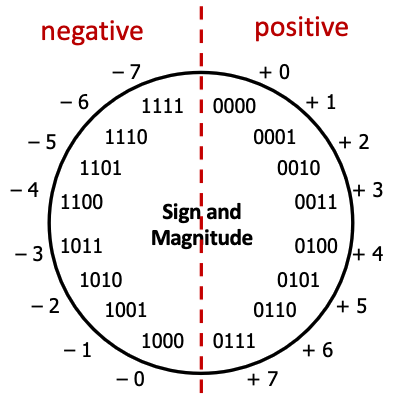
\includegraphics[scale=0.4]{img/signed_magnitude_encoding.png}
      \caption{Signed magnitude encoding of 4-bit integers in C.} 
      \label{fig:signed_magnitude_encoding}
    \end{figure}
    You can see that there are some problems: 
    \begin{enumerate}
      \item There are two representations for $0$, which is 0000 and 1000. 
      \item -1 (1001) plus 1 becomes -2 (1010). 
      \item The lowest number -7 (1111) plus 1 goes to 0 (0000) when it should go to -6 (1100). 
      \item The highest number 7 (0111) plus 1 goes to 0 (1000). 
    \end{enumerate}
  \end{example}

  An alternative way is to use the two's complement representation, which solves both problems and makes it more natural. 

  \begin{theorem}[Bit Representation of Signed Integers in C]
    The \textbf{two's complement} representation is a way to represent signed integers in binary. It is defined as follows. Given that you want to store a decimal number $p$ in $n$ bits, 

    \begin{enumerate}
      \item If $p$ is positive, then take the binary expansion of that number, which should be at most $n-1$ bits (no overflow), pad it with $0$s on the left. 
      \item If $p$ is negative, then you can do two things: First, take the binary expansion of the positive number, flip all the bits, and add 1. Or second, represent $p = q - 2^n$, take the binary representation of $q$ in $n-1$ bits, and add a $1$ to the left. 
    \end{enumerate}
    If you have a binary number $b = b_{n}b_{n-1}\cdots b_1$ then to convert it to a decimal number, you simply calculate 
    \begin{equation}
      q = -b_{n}2^{n-1} + b_{n-1}2^{n-2} + \cdots + b_1
    \end{equation}
    \begin{figure}[H]
      \centering 
      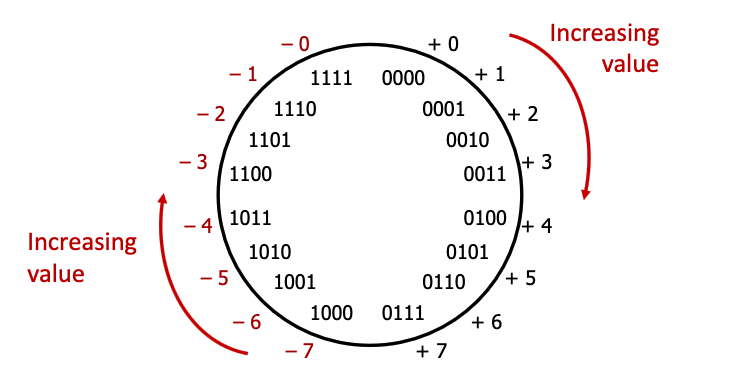
\includegraphics[scale=0.4]{img/twos_complement_encoding.png}
      \caption{Two's complement encoding of 4-bit integers in C.} 
      \label{fig:twos_complement_encoding}
    \end{figure}
  \end{theorem}

  \begin{example}[Bit Representation of Signed Integers in C]
    We can see for ourselves how these numbers are represented in bits. 

    \noindent\begin{minipage}{.5\textwidth}
    \begin{lstlisting}[]{Code}
      int main() { 

        short short_pos = 13; 
        short short_neg = -25; 
        int int_pos = 256;
        int int_neg = -512; 

        printf("%x\n", short_pos);
        printf("%x\n", short_neg);
        printf("%x\n", int_pos);
        printf("%x\n", int_neg);

        return 0; 
      }
    \end{lstlisting}
    \end{minipage}
    \hfill
    \begin{minipage}{.49\textwidth}
    \begin{lstlisting}[]{Output}
      d
      ffe7
      100
      ffffffe00
      .
      .
      .
      .
      .
      .
      .
      .
      .
      .
    \end{lstlisting}
    \end{minipage}
  \end{example}

  \begin{figure}[H]
    \centering 
    \noindent\begin{minipage}{.5\textwidth}
    \begin{lstlisting}[]{Code}
      #include<stdio.h>
      #include<stdbool.h>

      int main() {
        printf("%lu\n", sizeof(bool)); 
        printf("%lu\n", sizeof(short)); 
        printf("%lu\n", sizeof(int)); 
        printf("%lu\n", sizeof(long)); 
        printf("%lu\n", sizeof(long long)); 
        return 0; 
      }
    \end{lstlisting}
    \end{minipage}
    \hfill
    \begin{minipage}{.49\textwidth}
    \begin{lstlisting}[]{Output}
      1
      2
      4
      8
      8
      .
      .
      .
      .
      .
      .
    \end{lstlisting}
    \end{minipage}
    \caption{Size of various integer types in C with the \texttt{sizeof}.} 
    \label{fig:integer_size}
  \end{figure}


  \subsubsection{Arithmetic Operations on Binary Numbers}

    \begin{theorem}[Inversion of Binary Numbers]
      Given a binary number $p$, to compute $-p$, simply invert the bits and add 1.
    \end{theorem}

    \begin{theorem}[Addition and Subtraction of Binary Numbers]
      Given two binary numbers $p$ and $q$. 
      \begin{enumerate}
        \item To compute $p + q$, simply add the numbers together as you would in base 10, but carry over when the sum is greater than 1. 
        \item To compute $p - q$, you can invert $q$ to $-q$ and compute $p + (-q)$. 
      \end{enumerate}
    \end{theorem}

    % TODO: Bitshift and Bitwise Operations

\subsection{Rationals and Countable Sets}
  
  When representing rational numbers, we cannot simply concatenate the numerator and denominator as such
  \[a/b \mapsto ZtS(a) \, ZtS(b)\]
  since this map is not surjective (and may overlap with other integers). 

  \begin{definition}[Representation of Rationals]
    To represent a rational number $a/b$, we create a separator symbol $|$ and map the rational number as below in the alphabet $\{0, 1, |\}$. 
    \[q: a/b \mapsto ZtS(a) | ZtS(b)\]
    Then, we use a second map that goes through each digit in $z$ and is defined 
    \[p: \{0, 1, |\} \longrightarrow \{00,11,01\} \subset \{0, 1\}^2, \; p(n) = \begin{cases}
    00 & n = 0 \\
    11 & n = 1 \\
    01 & n = |
    \end{cases}\]
    Therefore, $p$ maps the length $n$ string $z \in \{0, 1\}^\ast$ to the length $2n$ string $\omega \in \{0, 1\}^\ast$. The representation scheme for $\mathbb{Q}$ is simply 
    \[QtS \equiv p \circ q\]
  \end{definition}

  \begin{example}
  Given the rational number $-5/8$,
  \[\frac{-5}{8} \mapsto 1101|01000 \mapsto 11110011010011000000\]
  \end{example}

  This same idea of using separators and compositions of injective functions can be used to represent arbitrary $n$-tuples of strings (since a finite Cartesian product of countable sets is also countable). 

  \begin{theorem}[Representation of Vectors]
    All vectors, matrices, and tensors over the field $\mathbb{Q}$ are representable. 
  \end{theorem}
  \begin{proof}
    For vectors, we can simply create another separator symbol $\cdot$ and have the initial mapping $q$ map to a string over the alphabet $\{0, 1, |, \cdot\}$, which injectively maps to $\{00, 01, 10, 11\}$. 
    For tensors, create more separator symbols and map them to a sufficiently large set (which can be extended arbitrarily). For example, to perhaps $\{000, 001, ..., 111\}$. 

  \end{proof}

  \begin{corollary}[Representation of Graphs]
    Directed graphs, which can be represented with their adjacency matrices, can therefore be represented with binary strings. 
  \end{corollary}

  \begin{theorem}[Representation of Images]
    Every finite-resolution image can be represented as a binary number. 
  \end{theorem}
  \begin{proof}
    Since we can interpret each image as a matrix where each element (a pixel) is a color, and since each color can be represented as a 3-tuple of rational numbers corresponding to the intensities of red, green, and blue (for humans, we can restrict it to three primary colors), all images can eventually be decomposed into binary strings. 
  \end{proof}

\subsection{Floats} 

  \begin{theorem}[Representation of Reals]
    There exists no representation of the reals
    \begin{equation}
      NtR: \mathbb{R} \longrightarrow \{0, 1\}^\ast
    \end{equation}
  \end{theorem}
  \begin{proof}
    By Cantor's theorem, the reals are uncountable. That is, there does not exist a surjective function $NtR: \mathbb{N} \longrightarrow \mathbb{R}$. The implies the nonexistence of an injective inverse; that is, there does not exist an injective function 
    \[RtS: \mathbb{R} \longrightarrow \{0,1\}^\ast\]
  \end{proof}

  However, since $\mathbb{Q}$ is dense in $\mathbb{R}$, we can approximate every real number $x$ by a rational number $a/b$ to arbitrary accuracy. There are multiple ways to construct these approximations (decimal approximation up to $k$th digit, finite continued fractions, truncated infinite series, etc.), but computers use the \textit{floating-point approximation}. 

  \begin{definition}[Floating-Point Representation]
    The \textbf{floating-point representation scheme} of a real number $x \in \mathbb{R}$ is its approximation as a number of the form 
    \[\sigma b \cdot 2^e\]
    where $\sigma \in \{0, 1\}$ determines the sign of the representation of $x$, $e$ is a (potentially negative) integer, and $b$ is a rational number between $1$ and $2$ expressed as a binary fraction 
    \[1.b_0 b_1 b_2 ... b_k = 1 + \frac{b_1}{2} + \frac{b_2}{4} + ... + \frac{b_k}{2^k}, \;\; b_i \in \{0,1\}\]
    where the number $k$ is fixed (determined by the desired accuracy; greater $k$ implies more digits and better accuracy). The $\sigma b \cdot 2^e$ closest to $x$ is the \textit{floating-point representation}, or \textit{approximation}, of $x$. We can think of $\sigma$ determining the sign, $e$ the order of magnitude (in base 2) of $x$, and $b$ the value of the number scaled down to a value in $[1,2)$, called the \textit{mantissa}. 
  \end{definition}

  \begin{definition}[Floating Point Types in C]
    In C, there are several floating point types. We use this hierarchical method to give flexibility to the programmer on the size of the integer and whether it is signed or not. 
    \begin{enumerate} 
      \item A \textbf{float} is 4 bytes long and can be represented as an 8-digit hex or 32 bits, with values in $[1.2 \times 10^{-38}: 3.4 \times 10^{38}]$. 
      \item A \textbf{double} is 8 bytes long and can be represented as an 16-digit hex or 64 bits, with values in $[2.3 \times 10^{-308}: 1.7 \times 10^{308}]$. 
      \item A \textbf{long double} is 8 bytes and can be represented as an 16-digit hex or 64 bits, but they are only guaranteed to be stored in 80 bits in other systems. 
    \end{enumerate}
  \end{definition}

  \begin{theorem}[Bit Representation of Floating Point Types in C]
    Floats are actually like signed magnitude. We have 
    \begin{equation} 
      (-1)^n \times 2^{e - 127} \times 1.s
    \end{equation}

    \begin{figure}[H]
      \centering 
      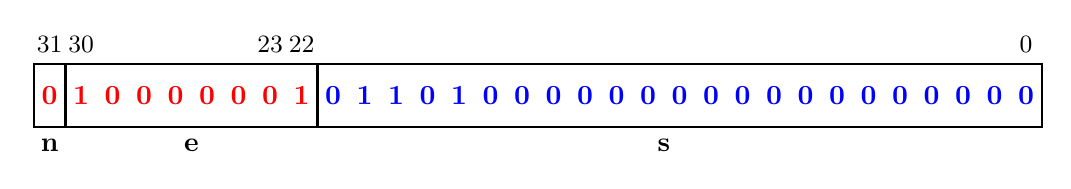
\begin{tikzpicture}[scale=0.8]
        % Draw the main box
        \draw[thick] (0,0) rectangle (16,1);
        
        % Vertical dividers
        \draw[thick] (0.5,0) -- (0.5,1);
        \draw[thick] (4.5,0) -- (4.5,1);
        
        % Bit numbers at top
        \node at (0.25,1.3) {\small 31};
        \node at (0.75,1.3) {\small 30};
        \node at (3.75,1.3) {\small 23};
        \node at (4.25,1.3) {\small 22};
        \node at (15.75,1.3) {\small 0};
        
        % Sign bit (red)
        \node[red] at (0.25,0.5) {\textbf{0}};
        
        % Exponent bits (red)
        \node[red] at (0.75,0.5) {\textbf{1}};
        \node[red] at (1.25,0.5) {\textbf{0}};
        \node[red] at (1.75,0.5) {\textbf{0}};
        \node[red] at (2.25,0.5) {\textbf{0}};
        \node[red] at (2.75,0.5) {\textbf{0}};
        \node[red] at (3.25,0.5) {\textbf{0}};
        \node[red] at (3.75,0.5) {\textbf{0}};
        \node[red] at (4.25,0.5) {\textbf{1}};
        
        % Mantissa bits (blue)
        \node[blue] at (4.75,0.5) {\textbf{0}};
        \node[blue] at (5.25,0.5) {\textbf{1}};
        \node[blue] at (5.75,0.5) {\textbf{1}};
        \node[blue] at (6.25,0.5) {\textbf{0}};
        \node[blue] at (6.75,0.5) {\textbf{1}};
        \node[blue] at (7.25,0.5) {\textbf{0}};
        \node[blue] at (7.75,0.5) {\textbf{0}};
        
        % Remaining zeros in light blue
        \foreach \x in {8.25,8.75,9.25,9.75,10.25,10.75,11.25,11.75,12.25,12.75,13.25,13.75,14.25,14.75,15.25,15.75} {
          \node[blue] at (\x,0.5) {\textbf{0}};
        }
        
        % Labels below
        \node at (0.25,-0.3) {\textbf{n}};
        \node at (2.5,-0.3) {\textbf{e}};
        \node at (10,-0.3) {\textbf{s}};
      \end{tikzpicture}
      \caption{32-bit representation of floats.} 
    \end{figure}

    Doubles encode 64 bits, so now we have exponent having 11 bits (so bias is not 1023) and 52 bits for mantissa. 
  \end{theorem}

\subsection{Characters}

  \begin{definition}[Booleans in C]
    The most basic type is the boolean, which is simply a bit. In C, it is represented as \texttt{bool}, and it is either \texttt{true} (1) or \texttt{false} (0). 
  \end{definition}

  We can manually check the size of the boolean type in C with the following code. 

  \begin{figure}[H]
    \centering 
    \noindent\begin{minipage}{.5\textwidth}
    \begin{lstlisting}[firstnumber=1]{Code}
      #include<stdio.h>
      #include<stdbool.h>

      int main() {
        printf("%lu\n", sizeof(bool)); 
        return 0; 
      }
    \end{lstlisting}
    \end{minipage}
    \hfill
    \begin{minipage}{.49\textwidth}
    \begin{lstlisting}[]{Output}
      1
      .
      .
      .
      .
      .
      .
    \end{lstlisting}
    \end{minipage}
    \caption{We can verify the size of various primitive data types in C with the \texttt{sizeof} operator.} 
    \label{fig:boolean_size}
  \end{figure}

  Note that \textbf{it does not make sense to have a string without knowing what encoding it uses}. We can't just assume that every plaintext is in ASCII, since there are hundreds of extended ASCII encodings. If you have a string, in memory, in a file, or in an email message, you have to know what encoding it is in or you cannot interpret it or display it to users correctly. 

  For example, when you are sending an email, Gmail is the only client that automatically converts your text to UTF-8, regardless of what you set in the header. The browser also uses a certain encoding, which can be accessed (and changed) under the "view" tab. 

  \subsubsection{ASCII}

    \begin{definition}[ASCII]
      The \textbf{ASCII} (also called US-ASCII) code, which stands for American Standard Code for Information Interchange is a $7$ bit character code where every single bit represents a unique character. ASCII codes represent text in computers, telecommunications equipment, and other devices. Most modern character-encoding schemes are based on ASCII, although they support many additional characters.

      The first 32 characters are called the \textit{control characters}: codes originally intended not to represent printable information, but rather to control devices (such as printers) that make use of ASCII, or to provide meta-information about data streams. For example, character 10 (decimal) represents the "line feed" function (which causes a printer to advance its paper) and character 8 represents "backspace." Except for the control characters that prescribe elementary line-oriented formatting, ASCII does not define any mechanism for describing the structure or appearance of text within a document. 
      \begin{center}
      \scalebox{0.8}{%
      \begin{tabular}{ |c|c|c|c|c|l| } 
        \hline
        Dec & Oct & Hex & Bin & Symbol & Description\\ 
        \hline
        0 & 000& 00& 0000000 & NULL & Null char\\ 
        1 & 001&01&0000001 & SOH & Start of Heading \\
        2 & 002 & 02 & 0000010& STX & Start of Text \\
        3 & 003 & 03 & 0000011&ETX & End of Text \\
        4 & 004 & 04 & 0000100 & EOT & End of Transmission \\
        5 & 005 & 05 & 0000101 & ENQ & Enquiry \\
        6 & 006 & 06 & 0000110 & ACK & Acknowledgement \\
        7 & 007 & 07 & 0000111 & BEL & Bell \\
        8 & 010 & 08 & 0001000 & BS & Back Space\\
        9 & 011 & 09 & 0001001 & HT & Horizontal Tab \\
        10 & 012 & 0A & 0001010 & LF & Line Feed \\
        11 & 013 & 0B & 0001011 & VT & Vertical Tab \\
        12 & 014 & 0C & 0001100 & FF & Form Feed\\
        13 & 015 & 0D & 0001101 & CR & Carriage Return \\
        14 & 016 & 0E & 0001110 & SO & Shift Out/X-On\\
        15 & 017 & 0F & 0001111 & SI & Shift In/X-Off\\
        16 & 020 & 10 & 0010000 & DLE & Data Line Escape\\
        17 & 021 & 11 & 0010001 & DC1 & Device Control 1\\
        18 & 022 & 12 & 0010010 & DC2 & Device Control 2\\
        19 & 023 & 13 & 0010011 & DC3 & Device Control 3\\
        20 & 024 & 14 & 0010100 & DC4 & Device Control 4 \\
        21 & 025 & 15 & 0010101 & NAK & Negative Acknowledgement\\
        22 & 026 & 16 & 0010110 & SYN & Synchronous Idle \\
        23 & 027 & 17 & 0010111 & ETB & End of Transmit Block\\
        24 & 030 & 18 & 0011000 & CAN & Cancel\\
        25 & 031 & 19 & 0011001 & EM & End of Medium\\
        26 & 032 & 1A & 0011010 & SUB & Substitute\\
        27 & 033 & 1B & 0011011 & ESC & Escape\\
        28 & 034 & 1C & 0011100 & FS & File Separator \\
        29 & 035 & 1D & 0011101 & GS & Group Separator\\
        30 & 036 & 1E & 0011110 & RS & Record Separator \\
        31 & 037 & 1F & 0011111 & US & Unit Separator\\
        \hline
      \end{tabular}}
      \end{center}

      The rest of the characters are the ASCII printable characters. 

      \scalebox{0.8}{%
      \begin{tabular}{ |c|c|c|c|c|l|c|c|c|c|c|l| } 
        \hline
        Dec & Oct & Hex & Bin & Sym & Description & Dec & Oct & Hex & Bin & Sym & Description \\
        \hline
        32 & 040 & 20& 0100000 &   & Space & 80 & 120 & 50& 1010000 &P&Uppercase P\\
        33 & 041 & 21& 0100001 & ! & Exclamation & 81 & 121 & 51& 1010001 &Q&Uppercase Q\\
        34 & 042 & 22& 0100010 & " & Double quotes & 82 & 122 & 52& 1010010 &R&Uppercase R\\
        35 & 043 & 23& 0100011 & \# & Number & 83 & 123 & 53& 1010011 &S&Uppercase S\\
        36 & 044 & 24& 0100100 & \$ & Dollar & 84 & 124 & 54& 1010100 &T&Uppercase T\\
        37 & 045 & 25& 0100101 & \% & Per cent sign & 85 & 125 & 55& 1010101 &U&Uppercase U\\
        38 & 046 & 26& 0100110 & \& & Ampersand & 86 & 126 & 56& 1010110 &V&Uppercase V\\
        39 & 047 & 27& 0100111 & ' &Single quote & 87 & 127 & 57& 1010111 &W&Uppercase W\\
        40 & 050 & 28& 0101000 & ( & Open paren.& 88 & 130 & 58& 1011000 &X&Uppercase X\\
        41 & 051 & 29& 0101001 & ) & Closed paren.& 89 & 131 & 59& 1011001 &Y&Uppercase Y\\
        42 & 052 & 2A& 0101010 & * & Asterisk & 90 & 132 & 5A& 1011010 &Z&Uppercase Z\\
        43 & 053 & 2B& 0101011 & + & Plus & 91 & 133 & 5B& 1011011 & [ & Opening bracket\\
        44 & 054 & 2C& 0101100 & , & Comma & 92 & 134 & 5C& 1011100 & \textbackslash & Backslash\\
        45 & 055 & 2D& 0101101 & - & Hyphen & 93 & 135 & 5D& 1011101 & ] & Closing bracket\\
        46 & 056 & 2E& 0101110 & . &Period & 94 & 136 & 5E& 1011110 & \string^ & Caret\\
        47 & 057 & 2F& 0101111 & / & Slash & 95 & 137 & 5F& 1011111 & \_ & Underscore\\
        48 & 060 & 30& 0110000 & 0 & Zero & 96 & 140 & 60& 1100000 &`&Grave accent\\
        49 & 061 & 31& 0110001 & 1 & One & 97 & 141 & 61& 1100001 &a& Lowercase a\\
        50 & 062 & 32& 0110010 & 2 & Two & 98 & 142 & 62& 1100010 &b&Lowercase b\\
        51 & 063 & 33& 0110011 & 3 & Three & 99 & 143 & 63& 1100011 &c&Lowercase c\\
        52 & 064 & 34& 0110100 & 4 & Four & 100 & 144 & 64& 1100100 &d&Lowercase d\\
        53 & 065 & 35& 0110101 & 5 & Five & 101 & 145 & 65& 1100101 &e&Lowercase e\\
        54 & 066 & 36& 0110110 & 6 & Six & 102 & 146 & 66& 1100110 &f&Lowercase f\\
        55 & 067 & 37& 0110111 & 7 & Seven & 103 & 147 & 67 &1100111 &g&Lowercase g\\
        56 & 070 & 38& 0111000 & 8 & Eight & 104 & 150 & 68& 1101000 &h&Lowercase h\\
        57 & 071 & 39& 0111001 & 9 & Nine & 105 & 151 & 69& 1101001 &i&Lowercase i\\
        58 & 072 & 3A& 0111010 & : & Colon & 106 & 152 & 6A& 1101010 &j&Lowercase j\\
        59 & 073 & 3B& 0111011 & ; & Semicolon & 107 & 153 & 6B& 1101011 &k&Lowercase k\\
        60 & 074 & 3C& 0111100 & < & Less than & 108 & 154 & 6C& 1101100 &l&Lowercase l\\
        61 & 075 & 3D& 0111101 & = & Equals & 109 & 155 & 6D& 1101101 &m&Lowercase m\\
        62 & 076 & 3E& 0111110 & > & Greater than & 110 & 156 & 6E& 1101110 &n&Lowercase n\\
        63 & 077 & 3F& 0111111 & ? & Question mark & 111 & 157 & 6F& 1101111 &o&Lowercase o\\
        64 & 100 & 40& 1000000 & @ & At symbol & 112 & 160 & 70& 1110000 &p&Lowercase p\\
        65 & 101 & 41& 1000001 & A & Uppercase A & 113 & 161 & 71& 1110001 &q&Lowercase q\\
        66 & 102 & 42& 1000010 & B& Uppercase B & 114 & 162 & 72& 1110010 &r&Lowercase r\\
        67 & 103 & 43& 1000011 &C&Uppercase C & 115 & 163 & 73& 1110011 &s&Lowercase s\\
        68 & 104 & 44& 1000100 &D&Uppercase D & 116 & 164 & 74& 1110100 &t&Lowercase t\\
        69 & 105 & 45& 1000101 &E&Uppercase E & 117 & 165 & 75& 1110101 &u&Lowercase u\\
        70 & 106 & 46& 1000110 &F&Uppercase F & 118 & 166 & 76& 1110110 &v&Lowercase v\\
        71 & 107 & 47& 1000111 &G&Uppercase G & 119 & 167 & 77& 1110111 &w&Lowercase w\\
        72 & 110 & 48& 1001000 &H&Uppercase H & 120 & 170 & 78& 1111000 &x&Lowercase x\\
        73 & 111 & 49& 1001001 &I&Uppercase I & 121 & 171 & 79& 1111001 &y&Lowercase y\\
        74 & 112 & 4A& 1001010 &J&Uppercase J & 122 & 172 & 7A& 1111010 &z&Lowercase z\\
        75 & 113 & 4B& 1001011 &J&Uppercase K & 123 & 173 & 7B& 1111011 &\{& Opening brace\\
        76 & 114 & 4C& 1001100 &L&Uppercase L & 124 & 174 & 7C& 1111100 &|& Vertical bar\\
        77 & 115 & 4D& 1001101 &M&Uppercase M & 125 & 175 & 7D& 1111101 &\}& Closing brace\\
        78 & 116 & 4E& 1001110 &N&Uppercase N & 126 & 176 & 7E& 1111110 & $\sim$ & Tilde\\
        79 & 117 & 4F& 1001111 &O&Uppercase O & 127 & 177 & 7F& 1111111 & & Delete\\
        \hline
      \end{tabular}}
    \end{definition}

    The \textbf{Extended ASCII} (EASCII or high ASCII) character encodings are 8-bit or larger encodings that include the standard 7-bit ASCII characters, plus additional characters. Note that this does not mean that the standard ASCII coding has been updated to include more than 128 characters nor does it mean that there is an universal extension to the original ASCII coding. In fact, there are several (over 100) extended ASCII encodings. 

    With the creation of the 7-bit ASCII format, increased need for more letters and symbols (such as characters in other languages or more punctuation/mathematical symbols). With better computers and software, it became obvious that they could handle text that uses 256-character sets at almost no additional cost in programming or storage. The 8-bit format would allow ASCII to be used unchanged and provide 128 more characters. 

    But even 256 characters is still not enough to cover all purposes, all languages, or even all European languages, so the emergence of \textit{many} ASCII-derived 8-bit character sets was inevitable. Translating between these sets (\textit{transcoding}) is complex, especially if a character is not in both sets and was often not done, producing \textbf{mojibake} (semi-readable text resulting from text being decoded using an unintended character encoding. The result is a systematic replacement of symbols with completely unrelated ones, often from a different writing system). ASCII can also be used to create graphics, commonly called \textbf{ASCII art}. 

    But ASCII isn't enough. We have lots of languages with lots of characters that computers should ideally display. Unicode assigns each character a unique number, or code print. Computers deal with such numbers as bytes: 8-bit computers would treat an 8-bit byte as the largest numerical unit easily represented on the hardware, 16-bit computers would expand that to 2 bytes, and so forth. Old character encodings like ASCII are from the (pre-) 8-bit era, and try to cram the dominant language in computing at the time, i.e. English, into numbers ranging from 0 to 127 (7 bits). When ASCII got extended by an 8th bit for other non-English languages, the additional 128 numbers/code points made available by this expansion would be mapped to different characters depending on the language being displayed. The \textbf{ISO-8859} standards are the most common forms of this mapping: 
    \begin{enumerate}
      \item \textbf{ISO-8859-1}
      \item \textbf{ISO-8859-15}, also called \textbf{ISO-Latin-1}
    \end{enumerate}
    But that's not enough when you want to represent characters from more than one language, so cramming all available characters into a single byte just won't work. The following shows ways to do this (that is compatible with ASCII). 

  \subsubsection{ISO-10646, UCS}

    We can simply expand the value range by adding more bits. The UCS-2 uses 2 bytes (or 16 bits) and UCS-4 uses 4 bytes (32 bits). However, these codings suffer from inherently the same problem as ASCII and ISO-8859 standards, as their value range is still limited, even if the limit is vastly higher. Note that these encode from the ISO-10646, which defines several character encoding forms for the Universal Coded Character Set. 
    \begin{enumerate}
        \item UCS-2 can store $2^{16} = 65,536$ characters. 
        \item UCS-4 can store $2^{32} = 4,294,967,296$ characters. 
    \end{enumerate}
    Notice that UCS encoding has a fixed number of bytes per character, which means that UCS-2 stores each character in 2 bytes, and UCS-4 stores each character in 4 bytes. This is different from \textbf{UTF-8} encoding. 

    ISO 10646 and Unicode have an identical repertoire and numbers—the same characters with the same numbers exist on both standards, although Unicode releases new versions and adds new characters more often. Unicode has rules and specifications outside the scope of ISO 10646. ISO 10646 is a simple character map, an extension of previous standards like ISO 8859. In contrast, Unicode adds rules for collation, normalization of forms, and the bidirectional algorithm for right-to-left scripts such as Arabic and Hebrew. For interoperability between platforms, especially if bidirectional scripts are used, it is not enough to support ISO 10646; Unicode must be implemented.

  \subsubsection{Unicode, UTF-8}

    Unicode is the universal character encoding, maintained by Unicode Consortium, and it covers the characters for all the writing systems of the world, modern and ancient. It also includes technical symbols, punctuation, and many other characters used in writing text. As of Unicode Version 13.0, the Unicode standard contains 143,859 characters, stored in the format U+****, where **** is a number in hexadecimal notation. Notice that these ones are not fixed in the number of bits; that is, 
    \[\text{U+27BD and U+1F886}\]
    are perfectly viable representations of characters in Unicode. Even though only 143,859 characters are in use, Unicode currently allows for 1,114,112 ($16^5 + 16^4$) code values, and assigns codes covering nearly all modern text writing systems, as well as many historical ones and for many non-linguistic characters such as printer's dingbats, mathematical symbols, etc.

    \textit{Note that Unicode, along with ISO-10646, is a standard that assigns a name and a value (\textbf{Character Code} or \textbf{Code-Point}) to each character in its repertoire.} However, the Unicode format must be encoded in a binary format for the computer to understand. When you save a document, the text editor has to explicitly set its encoding to be UTF-8 (or whatever other format) the user wants it to be. Also, when a text editor program reads a file, it needs to select a text encoding scheme to decode it correctly. Even further, when you are typing and entering a letter, the text editor needs to know what scheme you use so that it will save it correctly. Therefore, \textit{UTF-8 encoding is a way to represent these characters digitally in computer memory.} The way that \textbf{UTF-8} encodes characters is with the following format:
    \begin{lstlisting}
    1st Byte    2nd Byte    3rd Byte    4th Byte    Number of Free Bits   
    0xxxxxxx                                                7             
    110xxxxx    10xxxxxx                                (5+6)=11          
    1110xxxx    10xxxxxx    10xxxxxx                  (4+6+6)=16         
    11110xxx    10xxxxxx    10xxxxxx    10xxxxxx    (3+6+6+6)=21         
    \end{lstlisting}
    From this, we can see that UTF-8 uses a variable number of bytes per character. All UTF encodings work in roughly the same manner: you choose a unit size, which for UTF-8 is 8 bits, for UTF-16 is 16 bits, and for UTF-32 is 32 bits. The standard then defines a few of these bits as \textit{flags} (e.g. the 0, 110, 1110, 11110, ...). If they're set, then the next unit in a sequence of units is considered part of the same character. If they're not set, this unit represents one character fully. Thus, the most common (English) characters only occupy one byte in UTF-8 (two in UTF-16, 4 in UTF-32), but other language characters can occupy more bytes. We can see that UTF-8 can encode up to (and slightly more than) $2^{21} = 2,097,152$ characters. UTF-8 is by far the most common encoding for the World Wide Web, accounting for 96.0\% of all web pages, and up to 100\% for some languages, as of 2021.

    For example, let's take a random character, say with the Unicode value to be U+6C49. Then, we convert this to binary to get
    \[\text{01101100 01001001}\]
    But we can't just store this because this isn't a prefix-free notation. This is when UTF-8 is needed. Using the chart above, we need to prefix our character with some headers/flags. The binary Unicode value of the character is 16 bits long, so we can store it in 3 bytes (in the format of the third row) as it provides enough space. The headers are not bolded, while the binary values added are. 
    \[\text{1110}\textbf{0110} \; \text{10}\textbf{110001} \; \text{10}\textbf{001001}\]
    We can take another example of a character with the Unicode value U+1F886. Converting to binary gets
    \[\text{0001 1111 1000 1000 0110}\]
    There are 20 bits, so we will need to store it in 4 bytes (in the format of fourth row) as it provides enough space (21). We convert the 20-bit-long binary Unicode value to a 21-bit-long value (so that it is compatible with the 21 free bits) to get
    \[\text{0 0001 1111 1000 1000 0110}\]
    Encoding it in UTF-8 in 4 bytes gives
    \[\text{11110}\textbf{000} \; \text{10}\textbf{011111} \;  \text{10}\textbf{100010} \; \text{10}\textbf{000110}\]
    There is no need to go beyond 4 bytes since every Unicode value will have at most 5 hexadecimal digits (since $16^5 = 1,048,576$, which is far more than the number of characters there are). There is also another, obsolete, encoding used called the \textbf{UTF-7}. 

    Both the UCS and UTF standards encode the code points as defined in Unicode. In theory, those encodings could be used to encode any number (within the range the encoding supports) - but of course these encodings were made to encode Unicode code points. Windows handles so-called "Unicode" strings as UTF-16 strings, while most UNIXes default to UTF-8 these days. Communications protocols such as HTTP tend to work best with UTF-8, as the unit size in UTF-8 is the same as in ASCII, and most such protocols were designed in the ASCII era. On the other hand, UTF-16 gives the best average space/processing performance when representing all living languages. 

    While UTF-7, 8, 16, and 32 all have the nice property of being able to store \textit{any} code point correctly, there are hundreds of encodings that can only store a set amount of characters. If there’s no equivalent for the Unicode code point you’re trying to represent in the encoding you’re trying to represent it in, you usually get a little question mark: ? For example, trying to store Russian or Hebrew letters in these encodings results in a bunch of question marks. 

  \subsubsection{Text Files}

    The ASCII character set is the most common compatible subset of character sets for English-language text files, and is generally assumed to be the default file format in many situations. 

    In the Mac, checking the character encoding of a text file can be done with the command 
    \begin{lstlisting}
    >>>file -I filename.txt
    filename.txt: text/plain; charset=us-ascii
    \end{lstlisting}
    ASCII covers American English, but for the British Pound sign, the Euro sign, or characters used outside English, a richer character set must be used. In many systems, this is chosen based on the default setting on the computer it is read on. Prior to UTF-8, this was traditionally single-byte encodings (such as ISO-8859-1 through ISO-8859-16) for European languages and wide character encodings for Asian languages. However, most computers use UTF-8 as the natural extension. We can check this firsthand by inputting a non-ASCII character in filename.txt, which would result in
    \begin{lstlisting}
    >>>file -I filename.txt
    filename.txt: text/plain; charset=utf-8
    \end{lstlisting}
    Because encodings necessarily have only a limited repertoire of characters, often very small, many are only usable to represent text in a limited subset of human languages. Unicode is an attempt to create a common standard for representing all known languages, and most known character sets are subsets of the very large Unicode character set. Although there are multiple character encodings available for Unicode, the most common is UTF-8, which has the advantage of being backwards-compatible with ASCII; that is, every ASCII text file is also a UTF-8 text file with identical meaning. UTF-8 also has the advantage that it is easily auto-detectable. Thus, a common operating mode of UTF-8 capable software, when opening files of unknown encoding, is to try UTF-8 first and fall back to a locale dependent legacy encoding when it definitely isn't UTF-8.

    Because of their simplicity, text files are commonly used for storage of information. When data corruption occurs in a text file, it is often easier to recover and continue processing the remaining contents. A disadvantage of text files is that they usually have a low entropy, meaning that the information occupies more storage than is strictly necessary. A simple text file may need no additional metadata (other than knowledge of its character set) to assist the reader in interpretation. A text file may contain no data at all, which is a case of zero-byte file.

\subsection{Representation of General Sets}

  Let there exist some set $\mathcal{O}$ consisting of objects. Then, a representation scheme for representing objects in $\mathcal{O}$ consists of an \textit{encoding} function that maps an object in $\mathcal{O}$ to a string, and a \textit{decoding} function that decodes a string back to an object in $\mathcal{O}$. 

  \begin{definition}
  Let $\mathcal{O}$ be any set. A \textit{representation scheme for $\mathcal{O}$} is a pair of functions $E, D$ where 
  \[E: \mathcal{O} \longrightarrow \{0,1\}^\ast\]
  is an injective function, and the induced mapping $D$ is restriction of the inverse of $E$ to the image of $E$. 
  \[D: \mathrm{Im}(E) \subset \{0,1\}^\ast \longrightarrow \mathcal{O}\]
  This means that $(D \circ E) (o) = o$ for all $o \in \mathcal{O}$. $E$ is known as the \textit{encoding function} and $D$ is known as the \textit{decoding function}. 
  \end{definition}

  \begin{definition}[Prefix]
  For two strings $y, y^\prime$, $y$ is a prefix of $y^\prime$ if $y^\prime$ "starts" with $y$. That is, $y$ is a \textbf{prefix} of $y^\prime$ if $|y| \leq |y^\prime|$ and for every $i<|y|$, $y_i^\prime = y_i$. 
  \end{definition}

  With this, we can define the concept of prefix free encoding. 

  \begin{definition}
  Let $\mathcal{O}$ be a nonempty set and $E: \mathcal{O} \longrightarrow \{0,1\}^\ast$ be a function. $E$ is \textbf{prefix-free} if $E(o)$ is nonempty for every $o \in \mathcal{O}$ and there does not exist a distinct pair of objects $o, o^\prime \in \mathcal{O}$ such that $E(o)$ is a prefix of $E(o^\prime)$. 
  \end{definition}

  Being prefix-free is a nice property that we would like an encoding to have. Informally, this means that no string $x$ representing an object $o$ is an initial substring of string $y$ representing a different object $o$. This means that we can simply represent a \textit{list} of objects simply by concatenating the representations of all the list members and still get a valid, injective representation. We formalize this below.

  \begin{theorem}
  Suppose that $E: \mathcal{O} \longrightarrow \{0,1\}^\ast$ is prefix free. Then the following map 
  \[\overline{E}: \mathcal{O}^\ast \longrightarrow \{0,1\}^\ast\]
  over all finite length tuples of elements in $\mathcal{O}$ is injective, where for every $o_0, o_1, ..., o_{k-1} \in \mathcal{O}^\ast$, we define $\overline{E}$ to be the simple concatenation of the separate encodings of $o_i$: 
  \[\overline{E} (o_0, ..., o_{k-1}) \equiv E(o_0) E(o_1) ... E(o_{k-1})\]
  \end{theorem}

  Even if the representation $E$ of objects in $\mathcal{O}$ is prefix free, this does not imply that our representation $\overline{E}$ of \textit{lists} of such objects will be prefix free as well. In fact, it won't be, since for example, given three objects $o, o^\prime, o^{\prime\prime}$, the representation of the list $(o, o^\prime)$ will be a prefix of the representation of the list $(o, o^\prime, o^{\prime\prime})$.

  However, it turns out that in fact we can transform \textit{every} representation into prefix free form, and so will be able to use that transformation if needed to represents lists of lists, lists of lists of lists, and so on. 

  Some natural representations are prefix free. For example, every \textit{fixed output length} representation (i.e. an injective function $E: \mathcal{O} \longrightarrow \{0,1\}^n$) is automatically prefix-free, since a string $x$ can only be a prefix of an equal length $x^\prime$ if $x$ and $x^\prime$ are identical. Moreover, the approach that was used for representing rational numbers can be used to show the following lemma. 

  \begin{lemma}
  Let $E: \mathcal{O} \longrightarrow \{0,1\}^\ast$ be a one-to-one function. Then there is a one-to-one prefix-free encoding $\overline{E}$ such that 
  \begin{equation}
  | \overline{E}(o)| \leq 2 | E(o)| + 2
  \end{equation}
  for every $o \in \mathcal{O}$. 
  \end{lemma}
  \begin{proof}
  The general idea is the use the map $0 \mapsto 00$, $1 \mapsto 11$ to "double" every bit in the string $x$ and then mark the end of the string by concatenating to it the pair $01$. If we encode a string $x$ in this way, it ensures that the encoding of $x$ is never a prefix of the encoding of a distinct string $x^\prime$. (Note that this is not the only or even the best way to transform an arbitrary representation into prefix-free form.)
  \end{proof}


\section{Combinational Logic}

  Talk about how to construct arithmetic operations with these gates such as adding two integers or multiplying them, and not just that, but other operations that we may need in a programming language. 

\subsection{Multi-Bit Gates}

  Note that we can naturally work with multiple bits. This could mean a few things for---say, an AND gate. 
  \begin{enumerate}
    \item AND can take in multiple gates. 
    \item 
  \end{enumerate}

  \begin{definition}[Multi-Bit NOT Gate]
    
  \end{definition}

  \begin{definition}[Multi-Bit AND Gate]
    
  \end{definition}

  \begin{definition}[Multi-Bit OR Gate]
    
  \end{definition}

  \begin{definition}[Multi-Bit NAND Gate]
    
  \end{definition}

  \begin{definition}[Multi-Bit XOR Gate]
    
  \end{definition}

  \begin{definition}[Multi-Bit Multiplexor Gate]
    
  \end{definition}

  \begin{definition}[Multi-Bit Demultiplexor Gate]
    
  \end{definition}

\subsection{Addition and Subtraction} 

  We present a hierarchy of three adders, leading to a multi-bit adder chip. Note that every single chip here represents a finite function, and so from  \hyperref[th-thm:aon_univ]{universality of AON gates} we know that an implementation is definitely possible. 
  
  \begin{definition}[Half-Adder Chip] 
    A \textbf{half-adder} is designed to add two bits. 

    \begin{figure}[H]
      \centering
      \begin{subfigure}[b]{0.48\textwidth}
        \centering
        \begin{tabular}{|c|c||c|c|}
          \hline
          \multicolumn{2}{|c||}{\textbf{Inputs}} & \multicolumn{2}{c|}{\textbf{Outputs}} \\
          \hline
          \textbf{a} & \textbf{b} & \textbf{carry} & \textbf{sum} \\
          \hline
          0 & 0 & 0 & 0 \\
          \hline
          0 & 1 & 0 & 1 \\
          \hline
          1 & 0 & 0 & 1 \\
          \hline
          1 & 1 & 1 & 0 \\
          \hline
        \end{tabular}
        \caption{Truth table for half adder.}
      \end{subfigure}
      \hfill 
      \begin{subfigure}[b]{0.48\textwidth}
        \centering
        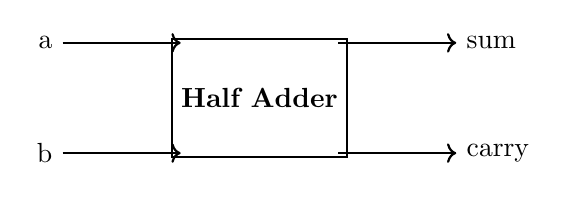
\begin{tikzpicture}
          % Block diagram
          \node[rectangle, draw, thick, minimum width=2cm, minimum height=1.5cm, font=\bfseries] 
              (halfadder) at (0, 0) {Half Adder};

          % Input lines
          \draw[thick, ->] (-2.5, 0.7) -- (-1, 0.7) node[left] at (-2.5, 0.7) {a};
          \draw[thick, ->] (-2.5, -0.7) -- (-1, -0.7) node[left] at (-2.5, -0.7) {b};

          % Output lines  
          \draw[thick, ->] (1, 0.7) -- (2.5, 0.7) node[right] at (2.5, 0.7) {sum};
          \draw[thick, ->] (1, -0.7) -- (2.5, -0.7) node[right] at (2.5, -0.7) {carry};
        \end{tikzpicture}
        \caption{}
      \end{subfigure}
      \caption{Chip diagram for half adder.}
    \end{figure}
  \end{definition}

  \begin{theorem}[Implementation of Half-Adder]
    To construct this chip, note that the way sum and carry acts on $a, b$ is identical to the standard $\XOR(a, b)$ and $\AND(a, b)$ functions. 

    \begin{figure}[H]
      \centering
      \begin{subfigure}[b]{0.48\textwidth}
        \centering
        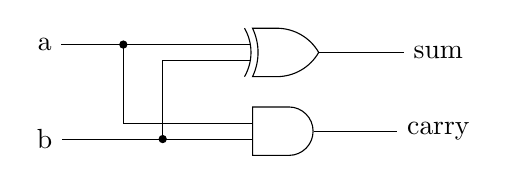
\begin{tikzpicture}[circuit logic US]
          % Input nodes
          \node (a) at (0,2.6) {a};
          \node (b) at (0,1.4) {b};

          % Logic gates
          \node[xor gate, draw] (xor1) at (3,2.5) {};
          \node[and gate, draw] (and1) at (3,1.5) {};

          % Output labels
          \node (sum) at (5,2.5) {sum};
          \node (carry) at (5,1.5) {carry};

          % Input connections
          \draw (a) -| (xor1.input 1);
          \draw (a) -- (1, 2.6) -- (1, 1.6) -| (and1.input 1);
          \draw (b) -- (1.5, 1.4) -- (1.5, 2.4) -| (xor1.input 2);
          \draw (b) -| (and1.input 2);

          % Output connections
          \draw (xor1.output) -- (sum);
          \draw (and1.output) -- (carry);

          % Add dots at connection points for clarity
          \fill (1.5,1.4) circle (1.5pt);
          \fill (1,2.6) circle (1.5pt);
        \end{tikzpicture}
        \caption{}
      \end{subfigure}
      \hfill 
      \begin{subfigure}[b]{0.48\textwidth}
        \centering
        \begin{lstlisting}
          module half_adder(
            input a, b, 
            output s, c
          ); 
            assign s = a ^ b;
            assign c = a & b;
          endmodule
        \end{lstlisting}
        \caption{HDL implementation.}
      \end{subfigure}
      \caption{}
    \end{figure}
  \end{theorem}

  \begin{definition}[Full-Adder] 
    Now that we know how to add two bits, a \textbf{full-adder chip}  allows us to add 3 bits. 

    \begin{figure}[H]
      \centering
      \begin{subfigure}[b]{0.48\textwidth}
        \centering
        \begin{tabular}{|c|c|c||c|c|}
          \hline
          \multicolumn{3}{|c||}{\textbf{Inputs}} & \multicolumn{2}{c|}{\textbf{Outputs}} \\
          \hline
          \textbf{a} & \textbf{b} & \textbf{cin} & \textbf{cout} & \textbf{sum} \\
          \hline
          0 & 0 & 0 & 0 & 0 \\
          \hline
          0 & 0 & 1 & 0 & 1 \\
          \hline
          0 & 1 & 0 & 0 & 1 \\
          \hline
          0 & 1 & 1 & 1 & 0 \\
          \hline
          1 & 0 & 0 & 0 & 1 \\
          \hline
          1 & 0 & 1 & 1 & 0 \\
          \hline
          1 & 1 & 0 & 1 & 0 \\
          \hline
          1 & 1 & 1 & 1 & 1 \\
          \hline
        \end{tabular}
        \caption{Truth table for full adder.}
      \end{subfigure}
      \hfill 
      \begin{subfigure}[b]{0.48\textwidth}
        \centering
        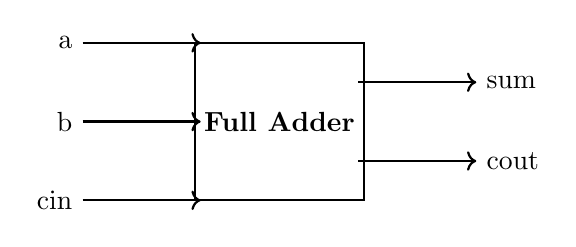
\begin{tikzpicture}
          % Block diagram
          \node[rectangle, draw, thick, minimum width=2cm, minimum height=2cm, font=\bfseries] 
              (fulladder) at (0, 0) {Full Adder};
          % Input lines
          \draw[thick, ->] (-2.5, 1) -- (-1, 1) node[left] at (-2.5, 1) {a};
          \draw[thick, ->] (-2.5, 0) -- (-1, 0) node[left] at (-2.5, 0) {b};
          \draw[thick, ->] (-2.5, -1) -- (-1, -1) node[left] at (-2.5, -1) {cin};
          % Output lines  
          \draw[thick, ->] (1, 0.5) -- (2.5, 0.5) node[right] at (2.5, 0.5) {sum};
          \draw[thick, ->] (1, -0.5) -- (2.5, -0.5) node[right] at (2.5, -0.5) {cout};
        \end{tikzpicture}
        \caption{Block diagram for full adder.}
      \end{subfigure}
      \caption{Chip diagram for full adder.}
    \end{figure}
  \end{definition}

  \begin{theorem}[Implementation of Full-Adder]
    We can implement a full adder with 2 half-adders and an $\OR$ gate. 

    \begin{figure}[H]
      \centering 
      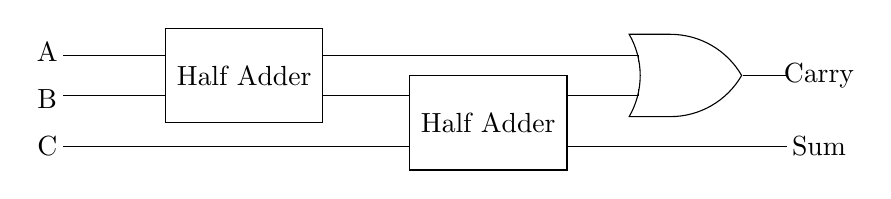
\begin{tikzpicture}[circuit logic US]
        % Input labels
        \node at (0, 2.8) {A};
        \node at (0, 2.2) {B};
        \node at (0, 1.6) {C};

        % First Half Adder
        \node[rectangle, draw, minimum width=2cm, minimum height=1.2cm] 
          (ha1) at (2.5, 2.5) {Half Adder};

        % Second Half Adder
        \node[rectangle, draw, minimum width=2cm, minimum height=1.2cm] 
          (ha2) at (5.6, 1.9) {Half Adder};

        \node[or gate, draw, scale=1.7] (or1) at (8, 2.5) {};

        \draw (0.2, 2.75) -- (1.5, 2.75);
        \draw (0.2, 2.25) -- (1.5, 2.25);
        \draw (0.2, 1.6) -- (4.6, 1.6);

        \draw (3.5, 2.75) -| (or1.input 1);
        \draw (3.5, 2.25) -- (4.6, 2.25);
        \draw (6.6, 2.25) -| (or1.input 2);
        \draw (or1.output) |- (9.4, 2.5);
        \draw (6.6, 1.6) -- (9.4, 1.6);
        \node at (9.8, 2.5) {Carry};
        \node at (9.8, 1.6) {Sum};
      \end{tikzpicture}
      \caption{} 
    \end{figure}
  \end{theorem}

  \begin{definition}[N-Bit Adder]
    Usually, $N$ is $16, 32, 64$, or $128$. 
  \end{definition}

  \begin{theorem}[Implementation of $N$-Bit Addition]

    \begin{figure}[H]
      \centering 
      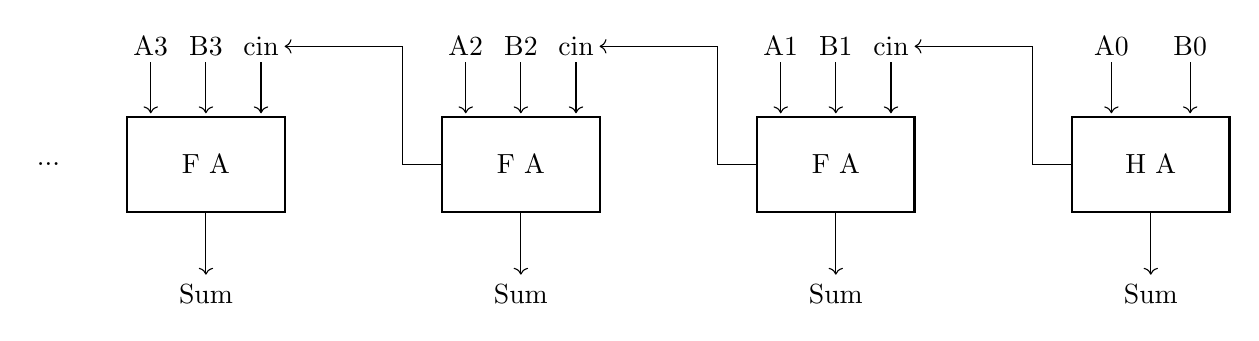
\begin{tikzpicture}
        % Input labels at the top
        \node at (1.3, 5) {A3};
        \node at (2, 5) {B3};
        \node at (2.7, 5) {cin};
        \draw[->] (1.3, 4.8) -- (1.3, 4.15);
        \draw[->] (2, 4.8) -- (2, 4.15);
        \draw[->] (2.7, 4.8) -- (2.7, 4.15);

        \node at (5.3, 5) {A2};
        \node at (6, 5) {B2};
        \node at (6.7, 5) {cin};
        \draw[->] (5.3, 4.8) -- (5.3, 4.15);
        \draw[->] (6, 4.8) -- (6, 4.15);
        \draw[->] (6.7, 4.8) -- (6.7, 4.15);

        \node at (9.3, 5) {A1};
        \node at (10, 5) {B1};
        \node at (10.7, 5) {cin};
        \draw[->] (9.3, 4.8) -- (9.3, 4.15);
        \draw[->] (10, 4.8) -- (10, 4.15);
        \draw[->] (10.7, 4.8) -- (10.7, 4.15);

        \node at (13.5, 5) {A0};
        \node at (14.5, 5) {B0};
        \draw[->] (13.5, 4.8) -- (13.5, 4.15);
        \draw[->] (14.5, 4.8) -- (14.5, 4.15);

        \node[rectangle, draw, thick, minimum width=2cm, minimum height=1.2cm] 
          (fa3) at (2, 3.5) {F A};
        \node[rectangle, draw, thick, minimum width=2cm, minimum height=1.2cm] 
          (fa2) at (6, 3.5) {F A};
        \node[rectangle, draw, thick, minimum width=2cm, minimum height=1.2cm] 
          (fa1) at (10, 3.5) {F A};
        \node[rectangle, draw, thick, minimum width=2cm, minimum height=1.2cm] 
          (ha0) at (14, 3.5) {H A};

        \draw[->] (2, 2.9) -- (2, 2.1);
        \node[below] at (2, 2.1) {Sum};

        \draw[->] (6, 2.9) -- (6, 2.1);
        \node[below] at (6, 2.1) {Sum};

        \draw[->] (10, 2.9) -- (10, 2.1);
        \node[below] at (10, 2.1) {Sum};

        \draw[->] (14, 2.9) -- (14, 2.1);
        \node[below] at (14, 2.1) {Sum};

        \draw[->] (13,3.5) -- (12.5, 3.5) -- (12.5, 5) -- (11, 5);
        \draw[->] (9,3.5) -- (8.5, 3.5) -- (8.5, 5) -- (7, 5);
        \draw[->] (5,3.5) -- (4.5, 3.5) -- (4.5, 5) -- (3, 5);
        \node at (0, 3.5) {...};
      \end{tikzpicture}
      \caption{Ripple carry adder for the last 4 significant bits of two $N$-bit numbers.} 
    \end{figure}
  \end{theorem}

  \begin{corollary}[Implemention for $N$-Bit Subtraction]
    
  \end{corollary}

  This is a standard construction and a goods start, but there are a few pitfalls of this. First, this does not detect nor handle overflows after adding. This will be handled at the operating system level. Second, addition is limited in that we can only apply it for precisely 2 arguments. 

  Ripple carry, carry select, carry look ahead adder to make it parallel (lecture 4)

  \begin{example}[More Arguments for Binary Addition]
    Note that the full adder---which takes in 3 bits---was designed so that there is enough space for each digit of the 2 inputs, plus a potential carry. If there were 3 inputs, then the full adder would need to support 4 inputs. Even worse, if we have $1 + 1 + 1 + 1 = 100$, then our carry digit will be greater than 1 digit, which messes things up even more. 
  \end{example}

  Finally, note that this is not a very efficient way to add because there are delays as the carry bit propagates from the least significant to the most significant bit pair. We can improve this with carry look-ahead techniques. 

\subsection{Multiplication} 

  Booths algo to do multiplication fast with bitshifts and addition 

  \begin{theorem}[Implementation of Bitshift Operations]
    
  \end{theorem}

  The reason bitshift is introduced first is that in binary, bit-shifting is equivalent to multiplication! 

  \begin{theorem}[Implementation of Multiplication in Circuits]
    
  \end{theorem}

  \begin{theorem}[Implementation of Moving Data in Circuits]
    
  \end{theorem}

\subsection{Arithmetic Logical Unit (ALU)}

\subsection{Conditionals}

  We also want some sort of conditionals. This then can be used to implement loops by checking some conditional. 

  \begin{theorem}[Implementation of Conditionals in Circuits]
    
  \end{theorem}



\section{Memory Banks}

  \begin{definition}[Memory]
    The \textbf{memory} is where the computer stores data and instructions, which can be though of as a giant array of memory addresses, with each containing a byte. This data consists of graphical things or even instructions to manipulate other data. It can be visualized  as a long array of boxes that each have an \textbf{address} (where it is located) and \textbf{contents} (what is stored in it).

    Memory simply works as a bunch of bits in your computer with each bit having some memory address, which is also a bit. For example, the memory address \texttt{0b0010} (2) may have the bit value of \texttt{0b1} (1) stored in it. 

    \begin{figure}[H]
      \centering 
      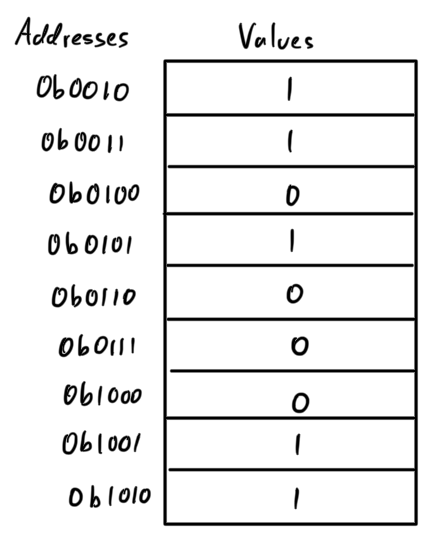
\includegraphics[scale=0.4]{img/memory_visual_bit.png}
      \caption{Visualization of memory as a long array of boxes of bits. }
      \label{fig:memory_visual_bit}
    \end{figure}

    However, computers do not need this fine grained level of control on the memory, and they really work at the Byte level rather than the bit level. Therefore, we can visualize the memory as a long array of boxes indexed by \textit{Bytes}, with each value being a byte as well. In short, the memory is \textbf{byte-addressable}. In certain arthitectures, some systems are \textbf{word-addressable}, meaning that the memory is addressed by words, which are 4 bytes.\footnote{Note that in here the size of a word is 2 bytes rather than 4 as stated above. This is just how it is defined in some \texttt{x86} architectures.}

    \begin{figure}[H]
      \centering 
      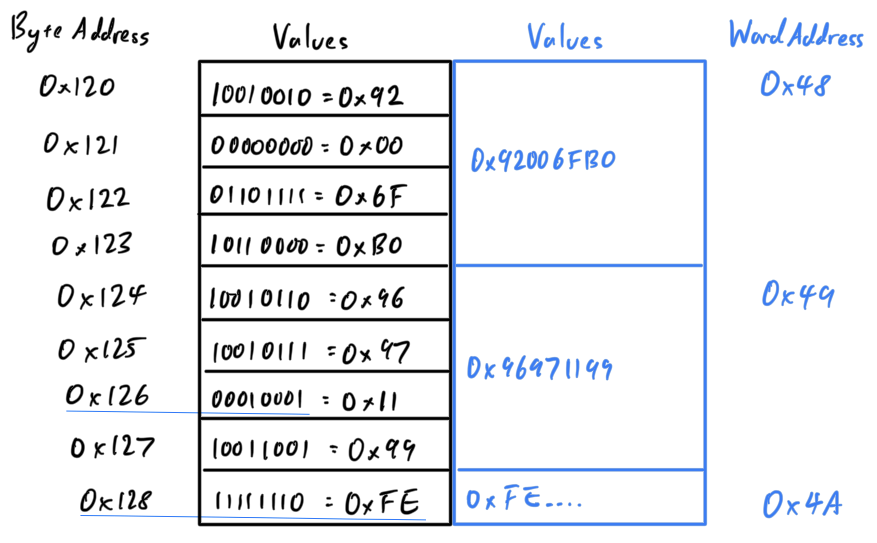
\includegraphics[scale=0.4]{img/memory_visual_byte.png}
      \caption{Visualization of memory as a long array of boxes of bytes. Every address is a byte and its corresponding value at that address is also a byte, though we represent it as a 2-digit hex. } 
      \label{fig:memory_visual_byte}
    \end{figure}
  \end{definition}

  It is intuitive to think that given some multi-byte object like an \texttt{int} (4 bytes), the beginning of the int would be the lowest address and the end of the int would be the highest address, like how consecutive integers are stored in an array. However, this is not always the case (almost always not the case since most computers are little-endian).  

  \begin{definition}[Endian Architecture]
    Depending on the machine architecture, computers may store these types slightly differently in their \textit{byte} order. Say that we have an integer of value \texttt{0xA1B2C3D4} (4 bytes). Then, 
    \begin{enumerate} 
      \item A \textbf{big-endian architecture} (e.g. SPARC, z/Architecture) will store it so that the least significant byte has the highest address.
      \item A \textbf{little-endian architecture} (e.g. x86, x86-64, RISC-V) will store it so that the least significant byte has the lowest address. 
      \item A \textbf{bi-endian architecture} (e.g. ARM, PowerPC) can specify the endianness as big or little. 
    \end{enumerate}

    \begin{figure}[H]
      \centering 
      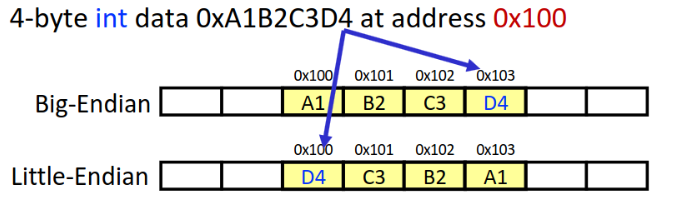
\includegraphics[scale=0.4]{img/endianness.png}
      \caption{The big vs little endian architectures. } 
      \label{fig:endianness}
    \end{figure}
  \end{definition}

  We can simply print out the hex values of primitive types to see how they are stored in memory, but it does not provide the level of details that we want on which bytes are stored where. At this point, we must use certain \textbf{debuggers} to directly look at the memory. For x86 architectures, we can use \texttt{gdb} and for ARM architectures, we can use \texttt{lldb}. At this point, we need to understand assembly to look through debuggers, so we will provide the example here. 

  To clarify, let us compare registers and memory. Memory is addressed by an unsigned integer while registers have names like \texttt{\%rsi}. Memory is much bigger at several GB, while the total register space is much smaller at around 128 bytes (may differ depending on the architecture). The memory is much slower than registers, which is usually on a sub-nanosecond timescale. The memory is dynamic and can grow as needed while the registers are static and cannot grow.


\section{Hardware Description Languages}

  Look into ternary operators, which is structural. Also for loops. 
  In gtkwave, look at edit/data,color format. 
  Select a bunch of wires and hit g to make a group. 

  Now that we know about chips, perhaps we are ready to mass produce them. Consider the following scenario where you are a hardware engineer with three boxes full of $\AND, \OR, \NOT$ gates. You need to ship an order of 1000 $\XOR$ gates. How would you do this? To construct one $\XOR$ gate, you can follow the example below. 

  \begin{figure}[H]
    \centering 
    \begin{tikzpicture}[circuit logic US]
      % Input nodes
      \node (a) at (0,3) {a};
      \node (b) at (0,1) {b};

      % NOT gates (top and bottom)
      \node[not gate, draw] (not1) at (2,2.5) {};
      \node[not gate, draw] (not2) at (2,1.5) {};

      % AND gates
      \node[and gate, draw] (and1) at (5,2.9) {};
      \node[and gate, draw] (and2) at (5,1.1) {};

      % OR gate
      \node[or gate, draw, logic gate inputs=nn] (or1) at (6,2) {};

      % Output node
      \node (out) at (7,2) {out};

      % Main input lines with junction dots
      \draw (a) -- (1,3) node[circle,fill,inner sep=1pt] {} -- (1.5,3);
      \draw (b) -- (1/5,1) node[circle,fill,inner sep=1pt] {} -- (1.5,1);

      % Connections from input a
      \draw (1,3) |- (not2.input);
      \draw (1,3) -- (3.5,3) |- (and1.input 1);

      % Connections from input b  
      \draw (1.5,1) |- (not1.input);
      \draw (1.5,1) -- (3.5,1) |- (and2.input 2);

      % NOT gate outputs to AND gates
      \draw (not1.output) |- (and1.input 2);
      \draw (not2.output) |- (and2.input 1);

      % AND gate outputs to OR gate with junction dots
      \draw (and1.output) |- (or1.input 1);
      \draw (and2.output) |- (or1.input 2);

      % Final output
      \draw (or1.output) -- (out);
    \end{tikzpicture}
    \caption{XOR Chip from AON gates.} 
    \label{fig:xor_from_aon}
  \end{figure}

  We would take two $\AND$ gates, two $\NOT$ gates, and one $\OR$ gate, mount them on a board according to the figure's layout, and connect the chips to one another by running copper wires among them and soldering the wire ends to the respective input/output pins. After this, we will have 3 exposed wire ends---two inputs and one output. We then solder a pin to each one of these wire ends, seal the entire device (except for the three pins) in a plastic encasing, and label it as $\XOR$. Do this 1000 times and you're done. 

  There's a lot of problems with this, with the foremost being that this might be error-prone, especially in more complex chips. There is guarantee that the given chip diagram is correct. Although we can prove correctness in simple cases like $\XOR$, we cannot do so in realistically complex chips. Thus, we need to empirically test the chip, i.e. connect it to a power supply, activate/deactivate the input pins in various configurations, and hope that the chip outputs will agree with its specifications. 

  Even this debugging process can be quite time-intensive if we endlessly tinker with wires and circuits. Therefore, engineers simulate the construction and testings of these circuits with \textbf{hardware simulators}. Remember that we have established that \textit{straight-line programs} are an equivalent model of finite computation, and so we can use lexical programs to model boolean circuits. These programs are called \textbf{hardware description languages (HDL)} (analogous to software language) and are used to model and design these digital systems. Once you have written a script in some HDL, you can use a \textbf{hardware simulator} (analogous to compiler) to test the circuit. We will use the Verilog language along with the Icarus Verilog hardware simulator.\footnote{Historically the \textit{VHDL} language was created as a military project---and is still in use---but is a bit ugly.  Then, \textit{Verilog} became the most dominant, but it has been largely replaced by \textit{SystemVerilog}. Regardless, both of these are a superset of Verilog, and we will begin with this. Given the Verilog language, \textit{Icarus Verilog} is its corresponding open-source hardware simulator that runs on all platforms (Windows, Mac, Linux).}

  \begin{definition}[Module]
    A \textbf{module} represents some sort of class. 
    \begin{enumerate}
      \item \textbf{Ports} represent the inputs and outputs of a gate, represented with the \texttt{input} and \texttt{output} keywords. You might see a convention to put the outputs first and then the inputs. 
      \item \textbf{Wires} are used for connecting different elements, like physical wires between gates. You can think of them as signals, which can be read (is current flowing?) or assigned, but no values get stored in them. They are automatically updated when input changes are specified with the \texttt{wire} keyword. 
      \item \textbf{Regs} are like variables that store values---similar to physical registers in CPUs. They are specified with the \texttt{reg} keyword. 
      \item The output value is determined by some logic using the \texttt{assign} keyword. 
    \end{enumerate}
  \end{definition}

\subsection{Structural and Behavioral Modeling}

  There are two paradigms of writing Verilog. \textbf{Structural modeling} refers to writing code in which we describe the \textit{structure}---i.e. each component---of our circuit. There are two main types. 

  \begin{figure}[H]
    \centering
    \begin{subfigure}[b]{0.48\textwidth}
      \centering
      \begin{lstlisting}
        module nand(
          input x1, x2,
          output y
        );
          wire z; 
          and and1(z, x1, x2); 
          not not1(y, z);
        endmodule
      \end{lstlisting}
      \caption{Gate level implementation.}
    \end{subfigure}
    \hfill 
    \begin{subfigure}[b]{0.48\textwidth}
      \centering
      \begin{lstlisting}
        module nand(
          input x1, x2,
          output y
        );
          assign y = ~(x1 & x2);


        endmodule
      \end{lstlisting}
      \caption{Dataflow level implementation.}
    \end{subfigure}
    \caption{Two different implementations of NAND. This example is just to show the difference between the two types of structural modeling. We will assume that NAND is the fundamental operator. }
  \end{figure}

  \begin{definition}[Gate Level Implementation]
    \textbf{Gate level implementation} is a functional paradigm similar to a straight line program. Here we use built-in \textbf{primitive gates} to work with bits, where the syntax is 
    \begin{lstlisting}
      gate gatename(*output, *input);
    \end{lstlisting}

    Here are some sample input signals for demonstration.
    \begin{lstlisting}
      reg a, b, c;
      wire out1, out2, out3, out4, out5, out6, out7, out8;
      wire out9, out10, out11, out12, out13, out14, out15; 
    \end{lstlisting}

    \begin{figure}[H]
      \centering
      \begin{subfigure}[b]{0.48\textwidth}
        \centering
        \begin{lstlisting}
          and  gate1(out1, a, b);
          or   gate2(out2, a, b);
          not  gate3(out3, a);   
          nand gate4(out4, a, b);
          nor  gate5(out5, a, b);
          xor  gate6(out6, a, b);
        \end{lstlisting}
        \caption{Basic logic gates.}
      \end{subfigure}
      \hfill 
      \begin{subfigure}[b]{0.48\textwidth}
        \centering
        \begin{lstlisting}
          and  gate8(out8, a, b, c);   
          or   gate9(out9, a, b, c);   
          nand gate10(out10, a, b, c); 
          nor  gate11(out11, a, b, c); 
          // XOR limited to 2 inputs
          .
        \end{lstlisting}
        \caption{Multiple input gates.}
      \end{subfigure}
      \caption{}
    \end{figure}
  \end{definition}

  \begin{definition}[Dataflow Modeling]
    \textbf{Dataflow modeling} models more of the flow of data, similar to mathematical notation. Here we use built-in \textbf{operators} rather than primitive gates. Here are some sample inputs for demonstration.
    \begin{lstlisting}
      reg [3:0] a = 4'b1010;
      reg [3:0] b = 4'b1100;
      reg [3:0] c;
    \end{lstlisting}
    There are many different types of operators one can use. 

    \begin{figure}[H]
      \centering
      \begin{subfigure}[b]{0.48\textwidth}
        \centering
        \begin{lstlisting}[language=Verilog]
          wire [3:0] and  = a & b;   
          wire [3:0] or   = a | b;   
          wire [3:0] not  = ~a;      
          wire [3:0] xor  = a ^ b;   
          wire [3:0] nand = ~(a & b);
          wire [3:0] nor  = ~(a | b);
          wire [3:0] xnor = ~(a ^ b);
        \end{lstlisting}
        \caption{Logical bitwise operators act on an array of bits and outputs an array.} 
      \end{subfigure}
      \hfill 
      \begin{subfigure}[b]{0.48\textwidth}
        \centering
        \begin{lstlisting}[language=Verilog]
          wire and  = &a;    
          wire or   = |a;    
          // not behaves identically
          wire xor  = ^a;    
          wire nand = ~&a;   
          wire nor  = ~|a;   
          wire xnor = ~^a;   
        \end{lstlisting}
        \caption{Reduction operators reduce an entire array to 1 bit, e.g. AND over $n$ inputs.}
      \end{subfigure}

      \begin{subfigure}[b]{0.48\textwidth}
        \centering
        \begin{lstlisting}[language=Verilog]
          wire [4:0] add_result = a + b;    
          wire [3:0] sub_result = a - b;    
          wire [7:0] mul_result = a * b;    
          wire [3:0] div_result = a 
          wire [3:0] mod_result = a % b;    

          wire logical_and = a && b;  
          wire logical_or  = a || b;  
          wire logical_not = !a;      
        \end{lstlisting}
        \caption{Arithmetic and logical operators}
      \end{subfigure}
      \hfill 
      \begin{subfigure}[b]{0.48\textwidth}
        \centering
        \begin{lstlisting}[language=Verilog]
          wire less_than         = a < b;   
          wire less_equal        = a <= b;  
          wire greater_than      = a > b;   
          wire greater_equal     = a >= b;  

          wire logical_equal     = a == b;  
          wire logical_not_equal = a != b;  
          wire case_equal        = a === b; 
          wire case_not_equal    = a !== b; 
        \end{lstlisting}
        \caption{Relational and equality operators.}
      \end{subfigure}
      \caption{}
    \end{figure}
  \end{definition}

  We will assume that the nand gate is always implemented. 

  \begin{definition}[Structural Implementation of AON]
    \begin{figure}[H]
      \centering 
      \begin{subfigure}[b]{0.32\textwidth}
        \centering
        \begin{lstlisting}
          module and(
            input x1, x2
            output y
          );
            wire z1;

            nand nand1(z1, x1, x2);
            nand nand2(y, z1, z1);

          endmodule
        \end{lstlisting}
        \caption{Gate Level AND}
      \end{subfigure}
      \hfill 
      \begin{subfigure}[b]{0.32\textwidth}
        \centering
        \begin{lstlisting}
          module or(
            input x1, x2, 
            output y
          ); 
            wire z1, z2;

            nand nand1(z1, x1, x1);
            nand nand2(z2, x2, x2); 
            nand nand3(y, z1, z2);
          endmodule
        \end{lstlisting}
        \caption{Gate Level OR}
      \end{subfigure}
      \hfill 
      \begin{subfigure}[b]{0.32\textwidth}
        \centering
        \begin{lstlisting}
          module not(
            input x, 
            output y
          ); 
            nand nand1(y, x, x);




          endmodule
        \end{lstlisting}
        \caption{Gate Level NOT}
      \end{subfigure}

      \begin{subfigure}[b]{0.32\textwidth}
        \centering
        \begin{lstlisting}
          module (
            input x1, x2, 
            output y
          ); 
            assign y = x1&x2;
          endmodule
        \end{lstlisting}
        \caption{Dataflow Level AND}
      \end{subfigure}
      \hfill 
      \begin{subfigure}[b]{0.32\textwidth}
        \centering
        \begin{lstlisting}
          module (
            input x1, x2, 
            output y
          ); 
            assign y = x1|x2
          endmodule
        \end{lstlisting}
        \caption{Dataflow Level OR}
      \end{subfigure}
      \hfill 
      \begin{subfigure}[b]{0.32\textwidth}
        \centering
        \begin{lstlisting}
          module (
            input x, 
            output y
          ); 
            assign y = ~x;
          endmodule
        \end{lstlisting}
        \caption{Dataflow Level NOT}
      \end{subfigure}

      \caption{Gate level implementations of elementary gates with NAND in Verilog (top). Notice that these look like straight line programs. Dataflow implementations make things more concise, but less readable.}
    \end{figure}
  \end{definition}

  \begin{definition}[Structural Implementation of NOR, XOR]
    \begin{figure}[H]
      \centering
      \begin{subfigure}[b]{0.48\textwidth}
        \centering
        \begin{lstlisting}
          
        \end{lstlisting}
        \caption{Gate Level NOR}
      \end{subfigure}
      \hfill 
      \begin{subfigure}[b]{0.48\textwidth}
        \centering
        \begin{lstlisting}
          
        \end{lstlisting}
        \caption{Gate Level XOR}
      \end{subfigure}

      \begin{subfigure}[b]{0.48\textwidth}
        \centering
        \begin{lstlisting}
          module nor(
            input x1, x2, 
            output y
          );
            assign y = ~(x1 | x2);
          endmodule
        \end{lstlisting}
        \caption{Dataflow Level NOR}
      \end{subfigure}
      \hfill 
      \begin{subfigure}[b]{0.48\textwidth}
        \centering
        \begin{lstlisting}
          module xor(
            input x1, x2, 
            output y
          );
            assign y = x1 ^ x2; 
          endmodule
        \end{lstlisting}
        \caption{Dataflow Level XOR}
      \end{subfigure}
      \caption{Gate level and dataflow level implementations in Verilog. }
    \end{figure}
  \end{definition}

  \begin{definition}[Structural Implementation of Multiplexor]
    \begin{figure}[H]
      \centering
      \begin{subfigure}[b]{0.48\textwidth}
        \centering
        \begin{lstlisting}
          module mux(a, b, x, out1); 
            input a, b, x; 
            output out1; 

            wire not_x; 
            wire out_and1, out_and2; 

            not not1(not_x, x); 
            and and1(out_and1, not_x, a); 
            and and2(out_and2, x, b); 
            or or1(out1, out_and1, out_and2); 
          endmodule
        \end{lstlisting}
        \caption{}
      \end{subfigure}
      \hfill 
      \begin{subfigure}[b]{0.48\textwidth}
        \centering
        \begin{lstlisting}
          module multiplex_gatel(a, b, x, out1); 
            input a, b, x; 
            output out1; 

            assign out1 = (~x & a)|(b & x);
          endmodule
        \end{lstlisting}
        \caption{}
      \end{subfigure}
      \caption{}
    \end{figure}
  \end{definition}

  Can be efficient but a bit cryptic. So we really want to describe the behavior of the circuit rather than what the circuit actually is. So we do not have to worry about the implementation details, and we trust that the compiler will take care of it. 

  \begin{example}[Behavioral Level Implementation of Multiplexor]
    In here, we don't care what the circuit looks like, and we model the behavior. 
    \begin{lstlisting}
      module multiplex_gate_level(A, B, X, out1); 
        input A, B, X; 
        output out1; 

        always @(*)
        begin
          if(X==0) 
            out1 = A; 
          else 
            out1 = B; 
        end
      endmodule
    \end{lstlisting}
  \end{example}

\subsection{Test Benching}

  We've seen how to construct certain gates/chips in Verilog, but we don't know if the circuits actually do what we want. For this, we need to set up \textit{test bench modules}. With these, we can select a predetermined set of inputs and test the signals through each intermediate wire and the output for each. 

  \begin{definition}[Test Bench Module]
    A \textbf{testbench module} represents a suite of inputs that you want to test. The \textbf{device under test (dut)} connects the testbench signals to the DUT ports using named port connections. 

    \begin{lstlisting}[language=Verilog]
      module nand_gate_tb;
        reg a, b; // registers that hold states
        wire y;

        // Instantiate device under test
        nand_gate dut(.a(a), .b(b), .y(y));

        initial begin
          // Enable waveform dumping
          $dumpfile("nand_gate.vcd");
          $dumpvars(0, nand_gate_tb);

          // Test all input combinations
          a = 0; b = 0; #10;
          a = 0; b = 1; #10;
          a = 1; b = 0; #10;
          a = 1; b = 1; #10;

          $display("Test complete");
          $finish;
        end

        // Monitor changes
        initial
          $monitor("At time %t: a=%b, b=%b, y=%b", $time, a, b, y);
      endmodule
    \end{lstlisting}
  \end{definition}

  \begin{example}[Test Benching Multiplexor]
    Here we show a testbench module that takes a predetermined set of inputs (all 8) and shows the signals traveling through each wire. 

    \begin{figure}[H]
      \centering 
      \begin{lstlisting}
        module tb_multiplex;
          reg A, B, X;
          wire out1;

          multiplex_gate uut(A, B, X, out1);

          initial begin
            // Test all combinations
            A = 0; B = 0; X = 0; #10;
            A = 0; B = 1; X = 0; #10;
            A = 1; B = 0; X = 0; #10;
            A = 1; B = 1; X = 0; #10;
            A = 0; B = 0; X = 1; #10;
            A = 0; B = 1; X = 1; #10;
            A = 1; B = 0; X = 1; #10;
            A = 1; B = 1; X = 1; #10;
            $finish;
          end

          initial begin
            $dumpfile("waves.vcd");
            $dumpvars(0, tb_multiplex);
          end
        endmodule
      \end{lstlisting}
      \caption{Test bench module for multiplexor in GTKwave.} 
    \end{figure}

    \begin{figure}[H]
      \centering 
      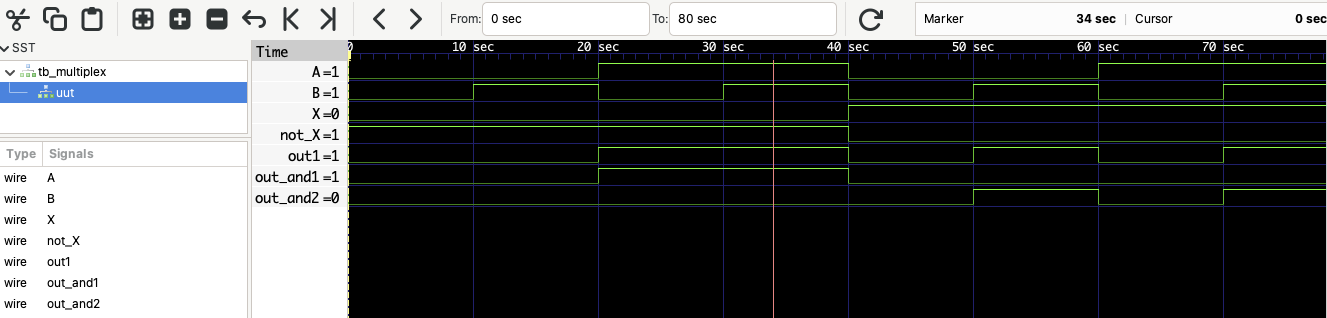
\includegraphics[scale=0.3]{img/multiplexor_gtk.png}
      \caption{View in GTKwave. You want to take a signal name in the bottom left and add it to the viewer by either double clicking on it or clicking ``append.''}
    \end{figure}
  \end{example}



\section{Instruction Sets} 

  \begin{definition}[Instruction Set]
    The \textbf{instruction set} of a CPU is ...
  \end{definition}

  Note that it only makes sense to talk about the instruction set architecture of some processing unit (e.g. CPU, GPU), and nothing more/less. It does not make sense to talk about the ISA of a computer, and it is usually implied that we are talking about the CPU residing \textit{in} the computer. 

\subsection{Addressing Modes}

  Registers being 8 bytes mean that we can store memory addresses, and if we can store memory addresses, we can access memory, i.e. the values at those memory addresses. There are 4 ways to do this, called \textbf{addressing modes}: immediate, normal, displacement, and indexed. When we parse an instruction, its operands are either 
  \begin{enumerate}
    \item Constant (literal) values 
    \item Registers 
    \item Memory forms
  \end{enumerate}

  \begin{definition}[Immediate Addressing]
    Immediate addressing is when the operand is a constant value, used with a \$ sign. 
    \begin{equation}
      \texttt{\$val}
    \end{equation}
  \end{definition}

  \begin{definition}[Normal Addressing]
    Normal addressing is when the operand is a register, used with a \% sign and the following syntax. The parentheses are used to dereference the memory address like dereferencing a pointer in C. 
    \begin{equation}
      \texttt{(R) = Mem[Reg[R]]}
    \end{equation}
    where \texttt{R} is the register name, \texttt{Reg[R]} is the value in the register, and \texttt{Mem[Reg[R]]} is the value in the memory address pointed to by the register. 
  \end{definition}

  \begin{definition}[Displacement Addressing]
    When we have a memory address stored in a register, we can add an offset to it to access a different memory address. 
    \begin{equation}
      \texttt{D(R) = Mem[Reg[R] + D]}
    \end{equation}
    where \texttt{R} is the register name and \texttt{D} is a constant displacement that specifies offset. 
  \end{definition}

  \begin{definition}[Indexed Addressing]
    Indexed addressing gives us more flexibility, allowing us to multiply the value in the register by a constant and add it to the value in another register. The general formula is shown as the top, but there are special cases: 
    \begin{align*}
      \texttt{D(Rb, Ri, S)} && = \texttt{Mem[Reg[Rb] + S*Reg[Ri] + D]} \\ 
      \texttt{D(Rb, Ri)} && = \texttt{Mem[Reg[Rb] + Reg[Ri] + D]} \\
      \texttt{(Rb, Ri, S)} && = \texttt{Mem[Reg[Rb] + S*Reg[Ri]]} \\ 
      \texttt{(Rb, Ri)} && = \texttt{Mem[Reg[Rb] + Reg[Ri]]} \\
      \texttt{(, Ri, S)} && = \texttt{Mem[S*Reg[Ri]]} 
    \end{align*}
    where \texttt{D} is a constant displacement of 1, 2, or 4 bytes, \texttt{Rb} is the base register (can be any of 8 integer registers), \texttt{Ri} is the index register (can be any register except \texttt{rsp}), and \texttt{S} is the scale factor (1, 2, 4, or 8). 
  \end{definition}

\subsection{Instructions}

    Now let's talk about how functions work on a deeper level. When we write a command, like \texttt{int x = 4}, we are manually looking for an address (in the stack, global, or heap) and rewriting the bits that are at that address. Functions are just an automated way to do this, and all these modifications and computations are done by the CPU. 

    \begin{definition}[Central Processing Unit]
      The CPU is responsible for taking instructions (data) from memory and executing them. 
      \begin{enumerate} 
        \item The CPU is composed of \textbf{registers} (different from the cache), which are small, fast storage locations. These registers can either be \textbf{general purpose} (can be used with most instructions) or \textbf{special purpose} (can be accessed through special instructions, or have special meanings/uses, or are simply faster when used in a specific way).
        \item The CPU also has an \textbf{arithmetic unit} and \textbf{logic unit}, which is responsible for performing arithmetic and logical operations. 
        \item The CPU also has a \textbf{control unit}, which is responsible for fetching instructions from memory through the \textbf{databus}, which is literally a wire connecting the CPU and RAM, and executing them. 
      \end{enumerate}
      It executes instructions from memory one at a time and executes them, known as the \textbf{fetch-execute cycle}. It consists of 4 main operations. 
      \begin{enumerate} 
        \item \textbf{Fetch}: The \textbf{program counter}, which holds the memory address of the next instruction to be executed, tells the control unit to fetch the instruction from memory through the databus. 
        \item \textbf{Decode}: The fetched data is passed to the \textbf{instruction decoder}, which figures out what the instruction is and what it does and stores them in the registers.
        \item \textbf{Execute}: The arithmetic and logic unit then carries out these operations. 
        \item \textbf{Store}: Then it puts the results back on the databus, and stores them back into memory.
      \end{enumerate} 
      The CPU's \textbf{clock cycle} is the time it takes for the CPU to execute one instruction. More specifically, the clock cycle refers to a single oscillation of the clock signal that synchronizes the operations of the processor and the memory (e.g. fetch, decode, execute, store), and decent computers have clock cycles of at least $2.60$GHz (2.6 billion clock cycles per second). 
    \end{definition}

    Therefore, in order to actually do computations on the data stored in the memory, the CPU must first fetch the data, perform the computations, and then store the results back into memory. This can be done in two ways.

    \begin{enumerate}
      \item Load and Store Operations: CPUs use load instructions to move data from memory to registers (where operations can be performed more quickly) and store instructions to move the modified data back into memory.
      \item If the data is too big to fit into the registers, the CPU will use the \textbf{cache} to store the data, and in worse cases, the actual memory itself. Compilers optimize code by maximizing the use of registers for operations to minimize slow memory access. This is why you often see assembly code doing a lot in registers.
    \end{enumerate}

    To clarify, let us compare registers and memory. Memory is addressed by an unsigned integer while registers have names like \texttt{\%rsi}. Memory is much bigger at several GB, while the total register space is much smaller at around 128 bytes (may differ depending on the architecture). The memory is much slower than registers, which is usually on a sub-nanosecond timescale. The memory is dynamic and can grow as needed while the registers are static and cannot grow.

    The specific structure/architecture of the CPU is determined by the instruction set architecture (ISA), which can be thought of as a subset of the general computer architecture. 

    \begin{definition}[Instruction Set Architecture]
      The \textbf{ISA} or just \textbf{architecture} of a CPU is a high level description of what it can do. Some differences are listed here: 
      \begin{enumerate} 
        \item What instructions it can execute. 
        \item The instruction length and decoding, along with its complexity. 
        \item The performance vs power efficiency. 
      \end{enumerate}
      ISAs can be classified into two types. 
      \begin{enumerate} 
        \item The \textbf{complex instruction set computer} (CISC) is characterized by a large set of complex instructions, which can execute a variety of low-level operations. This approach aims to reduce the number of instructions per program, attempting to achieve higher efficiency by performing more operations with fewer instructions.
        \item The \textbf{reduced instruction set computer} (RISC) emphasizes simplicity and efficiency with a smaller number of instructions that are generally simpler and more uniform in size and format. This approach facilitates faster instruction execution and easier pipelining, with the philosophy that simpler instructions can provide greater performance when optimized.
      \end{enumerate}
    \end{definition}

  \subsection{Instructions} 

      Now that we've gotten a sense of what these registers are and some commonalities between them, let's do some operations on them with instructions. 

      \begin{definition}[Instruction]
        An instruction is a single line of assembly code. It consists of some instruction followed by its (one or more) operands. The instruction is a mnemonic for a machine language operation (e.g. \texttt{mov}, \texttt{add}, \texttt{sub}, \texttt{jmp}, etc.). The \textbf{size specifier} can be appended to this instruction mnemonic to specify the size of the operands. 
        \begin{enumerate} 
          \item \textbf{b} (byte) for 1 byte 
          \item \textbf{w} (word) for 2 bytes
          \item \textbf{l} (long) for 4 bytes 
          \item \textbf{q} (quad word) for 8 bytes
        \end{enumerate}
        Note that due to backwards compatibility, word means 2 bytes in instruction names. Furthermore, the maximum size is 8 bytes since that is the size of each register in x86\_64. An operand can be of 3 types, determined by their \textbf{mode of access}:
        \begin{enumerate} 
          \item \textbf{Immediate addressing} is denoted with a \texttt{\$} sign, e.g. a constant integer data \texttt{\$1}. 
          \item \textbf{Register addressing} is denoted with a \texttt{\%} sign with the following register name, e.g. \texttt{\%rax}.
          \item \textbf{Memory addressing} is denoted with the hexadecimal address in memory, e.g. \texttt{0x034AB}.
        \end{enumerate}
      \end{definition}

      Like higher level programming languages, we can perform operations, do comparisons, and jump to different parts of the code. Instructions can be generally categorized into three types: 
      \begin{enumerate} 
        \item \textbf{Data Movement}: These instructions move data between memory and registers or between the registery and registery. Memory to memory transfer cannot be done with a single instruction. 
          \begin{lstlisting} 
            %reg = Mem[address]     # load data from memory into register
            Mem[address] = %reg     # store register data into memory
          \end{lstlisting}
        \item \textbf{Arithmetic Operation}: Perform arithmetic operation on register or memory data. 
          \begin{lstlisting} 
            %reg = %reg + Mem[address]     # add memory data to register
            %reg = %reg - Mem[address]     # subtract memory data from register
            %reg = %reg * Mem[address]     # multiply memory data to register
            %reg = %reg / Mem[address]     # divide memory data from register
          \end{lstlisting}
        \item \textbf{Control Flow}: What instruction to execute next both unconditional and conditional (if statements) ones. With if statements, loops can then be defined. 
          \begin{lstlisting} 
            jmp label     # jump to label
            je label      # jump to label if equal
            jne label     # jump to label if not equal
            jg label      # jump to label if greater
            jl label      # jump to label if less
            call label    # call a function
            ret           # return from a function
          \end{lstlisting}
      \end{enumerate}

      Now unlike compiled languages, which are translated into machine code by a compiler, assembly code is translated into machine code through a two-step process. First, we \textbf{assemble} the assembly code into an \textbf{object file} by an \textbf{assembler}, and then we \textbf{link} the object file into an executable by a \textbf{linker}. Some common assemblers are \textbf{NASM} (Netwide Assembler) and \textbf{GAS/AS} (GNU Assembler), and common linkers are \textbf{ld} (GNU Linker) and \textbf{lld} (LLVM Linker), both installable with \textbf{sudo pacman -S nasm ld}. 

    \subsubsection{Moving and Arithmetic} 

      Again, it is more important to have a general feel of what instructions every assembly language should  and get the ideas down rather than the syntax. We list them here, beginning with simply moving. 


      \begin{definition}[Moving]
        
      \end{definition}

      Next we want to have some sort of arithmetic to do calculations and to compare values. 

      \begin{definition}[Arithmetic Operations]
        
      \end{definition}

    \subsubsection{Conditionals}

      \begin{definition}[Conditionals]
        
      \end{definition}

    \subsubsection{Control Transfer on Stack}

      These are really the three basic functions needed to do anything in assembly, but let's talk about an important implementation called the \textbf{control transfer}. Say that you want to compute a function. 
      \begin{enumerate}
        \item Then we must retrieve the data from the memory. 
        \item We must load it into our registers in the CPU and perform some computation. 
        \item Then we must store the data back into memory. 
      \end{enumerate}

      Let’s begin with a refresher on how the call stack is managed. Recall that \texttt{\%rsp} is the stack pointer and always points to the top of the stack. The register \texttt{\%rbp} represents the base pointer (also known as the frame pointer) and points to the base of the current stack frame. The stack frame (also known as the activation frame or the activation record) refers to the portion of the stack allocated to a single function call. The currently executing function is always at the top of the stack, and its stack frame is referred to as the active frame. The active frame is bounded by the stack pointer (at the top of stack) and the frame pointer (at the bottom of the frame). The activation record typically holds local variables for a function.

      \begin{figure}[H]
        \centering 
        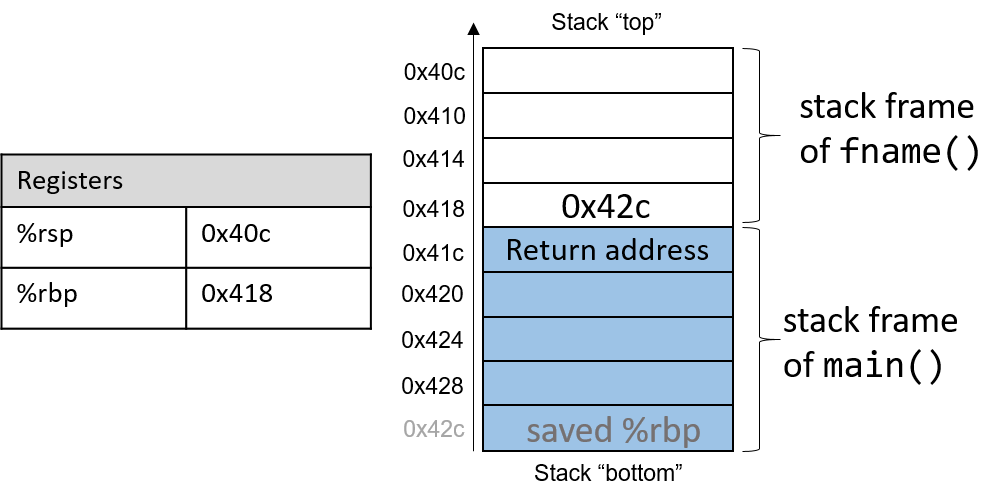
\includegraphics[scale=0.6]{img/stackFrame.png}
        \caption{The current active frame belongs to the callee function (fname). The memory between the stack pointer and the frame pointer is used for local variables. The stack pointer moves as local values are pushed and popped from the stack. In contrast, the frame pointer remains relatively constant, pointing to the beginning (the bottom) of the current stack frame. As a result, compilers like GCC commonly reference values on the stack relative to the frame pointer. In Figure 1, the active frame is bounded below by the base pointer of fname, which is stack address 0x418. The value stored at address 0x418 is the "saved" \texttt{\%rbp} value (0x42c), which itself is an address that indicates the bottom of the activation frame for the main function. The top of the activation frame of main is bounded by the return address, which indicates where in the main function program execution resumes once the callee function fname finishes executing. }
        \label{fig:stack_frame_management}
      \end{figure}


      Once we have done this we are really done. Formally, this is called Turing complete (?). 

      \begin{definition}[Control Transfers]
        We list some. 
        \begin{enumerate}
          \item Push 
          \item Pop 
          \item Call to call a function 
          \item Return to return from a function 
          \item Continue 
          \item Get out of stack with leave.  
        \end{enumerate}
      \end{definition}

      \begin{example}[Control Transfer Example]
        We show this with a minimal example with psuedocode. 
      \end{example}

    \subsubsection{Multiple Functions}

      Now what happens if there are multiple functions calling each other? Take a look at the following example with two functions. 

      \begin{example}[Multiple Functions Example]
        
      \end{example}

      There is a bit of a concern here from the previous example. The main function had two functions that returned two values. As the subfunction stack frame is removed from the stack, the return value is stored in the \texttt{\%rax} register. If another function is called right after, then the return value of the second function will overwrite that of the previous one. This was not a problem in the previous example since the return value of the \texttt{assign} function was not used. However, if it was, then the return value of the \texttt{adder} function would have overwritten it. This is known as register saving. 
      \begin{enumerate}
        \item For \textbf{caller-saved registers}, the caller function is responsible for saving the value of the register before calling a function and restoring it after the function returns. The caller should save values in its stack frame before calling the callee function, e.g. by pushing all the return values of each callee in the caller stack frame. Then it will restore values after the call. 

        \begin{center}
          \textit{Therefore, if we have a set of registers $\{\texttt{\%reg}\}$, the caller must take everything and push them in the caller stack frame. Then it will restore them after the call.}
        \end{center}

        \item For \textbf{callee-saved registers}, it is the callee's responsibility to save any data in these registers before using the registers. 

          \begin{center} 
            \textit{Therefore, if we have a set of registers $\{\texttt{\%reg}\}$, then inside the callee stack frame, the callee must take everything and push them in the callee stack frame. Once it computes the final return value, then it will restore all the saved register values from the callee stack frame back into the registers for the caller to use.}
          \end{center}
      \end{enumerate}

      Ideally, we want \textit{one} calling convention to simply separate implementation details between caller and callee. In general, however, neither is best. If the caller isn't using a register, then caller-save is better, and if callee doesn't need a register, then callee-save is better. If we do need to save, then callee save generally makes smaller programs, so we compromise and use a combination of both caller-save and callee-save. 




\section{Caches} 

  In order to actually do computations on the data stored in the memory, the CPU must first fetch the data, perform the computations, and then store the results back into memory. This can be done in two ways.

  \begin{enumerate}
    \item Load and Store Operations: CPUs use load instructions to move data from memory to registers (where operations can be performed more quickly) and store instructions to move the modified data back into memory.
    \item If the data is too big to fit into the registers, the CPU will use the \textbf{cache} to store the data, and in worse cases, the actual memory itself. Compilers optimize code by maximizing the use of registers for operations to minimize slow memory access. This is why you often see assembly code doing a lot in registers.
  \end{enumerate}

\subsection{Locality}

  So far, we have abstracted away most of these memory types as a single entity with nearly instantaneous access, but in practice this is not the case. The most simple way is to simply have RAM and our CPU registers, but by introducing more intermediate memory types, we can achieve greater efficiency. 

  \begin{definition}[Locality]
    \textbf{Locality} is a principle that generally states that a program that accesses a memory location $n$ at time $t$ is likely to access memory location $n + \epsilon$ at time $t + \epsilon$. This principle motivates the design of efficient caches. 
    \begin{enumerate}
      \item \textbf{Temporal locality} is the idea that if you access a memory location, you are likely to access it again soon. 
      \item \textbf{Spatial locality} is the idea that if you access a memory location, you are likely to access nearby memory locations soon.
    \end{enumerate}
    This generally means that if you access some sort of memory, the values around that address is also likely to be accessed and therefore it is wise to store it closer to your CPU. In CPUs, both the instructions and the data are stored in the cache, which exploits both kinds of locality (repeated operations for temporal and nearby data for spatial). 
  \end{definition}

  \begin{example}[Locality]
    Consider the following code. 
    \begin{lstlisting}
      int sum_array(int *array, int len) {
        int i;
        int sum = 0;

        for (i = 0; i < len; i++) {
          sum += array[i];
        }

        return sum;
      }
    \end{lstlisting}
    \begin{enumerate}
      \item \textbf{Temporal Locality}
        \begin{enumerate}
          \item We cycle through each loop repeatedly with the same add operation, exploiting temporal locality.  
          \item The CPU accesses the same memory (stored in variables \texttt{i}, \texttt{len}, \texttt{sum}, \texttt{array}) within each iteration and therefore at similar times. 
        \end{enumerate}
      \item \textbf{Spatial Locality}
        \begin{enumerate}
          \item The spatial locality is exploited when the CPU accesses memory locations from each element of the array, which are contiguous in memory. 
          \item Even though the program accesses each array element only once, a modern system loads more than one \texttt{int} at a time from memory to the CPU cache. That is, accessing the first array index fills the cache with not only the first integer but also the next few integers after it too. Exactly how many additional integers get moved depends on the cache's \textbf{block size}. For example, a cache with a 16 byte block size will store \texttt{array[i]} and the elements in \texttt{i+1}, \texttt{i+2}, \texttt{i+3}. 
        \end{enumerate}
    \end{enumerate}
  \end{example}

  We can see the differences in spatial locality in the following example. 

  \begin{example}
    One may find that simply changing the order of loops can cause a significant speed up in your program. Consider the following code. 
    \begin{figure}[H]
      \centering 
      \noindent\begin{minipage}{.5\textwidth}
      \begin{lstlisting}[]{Code}
        float averageMat_v1(int **mat, int n) {
          int i, j, total = 0;

          for (i = 0; i < n; i++) {
            for (j = 0; j < n; j++) {
              // Note indexing: [i][j]
              total += mat[i][j];
            }
          }
          return (float) total / (n * n);
        }
      \end{lstlisting}
      \end{minipage}
      \hfill
      \begin{minipage}{.49\textwidth}
      \begin{lstlisting}[]{Output}
        float averageMat_v2(int **mat, int n) {
          int i, j, total = 0;

          for (j = 0; j < n; j++) {
            for (i = 0; i < n; i++) {
              total += mat[i][j];
            }
          }
          return (float) total / (n * n);
        }
        .
      \end{lstlisting}
      \end{minipage}
      \caption{Two implementations of taking the total sum of all elements in a matrix.} 
      \label{fig:matrix_sum}
    \end{figure}
    It turns out that the left hand side of the code executes about 5 times faster than the second version. Consider why. When we iterate through the \texttt{i} first and then the \texttt{j}, we access the values \texttt{array[i][j]} and then by spatial locality, the next few values in the array, which are \texttt{array[i][j+1]}, ... are stored in the cache. 
    \begin{enumerate}
      \item In the left hand side of the code, these next stored values are exactly what is being accessed, and the CPU can access them in the cache rather than having to go into memory. 
      \item In the right hand side of the code, these next values are \textit{not} being accessed since we want to access \texttt{array[i+1][j]}, .... Unfortunately, this is not stored in the cache and so for every $n^2$ loops we have to go back to the memory to retrieve it. 
    \end{enumerate}
  \end{example}

\subsection{Caches}

  In theory, a cache should know which subsets of a program's memory it should hold, when it should copy a subset of a program's data from main memory to the cache (or vice versa), and how it can determine whether a program's data is present in the cache. Let's talk about the third point first. It all starts off with a CPU requesting some memory address, and we want to determine whether it is in the cache or not. To do this, we need to look a little deeper into memory addresses. 

  \begin{definition}[Portions of Memory Addresses]
    A memory address is a $m$-bit number.\footnote{64 in 64-bit machines.} It is divided up into three portions. 
    \begin{enumerate}
      \item The \textbf{tag} field with $t$ bits at the beginning.
      \item The \textbf{index} field with $i$ bits in the middle. 
      \item The \textbf{offset} field with $o$ bits at the end.
    \end{enumerate}
    The tag plus the index together refers to the \textbf{block number}. 
    \begin{figure}[H]
      \centering 
      \begin{tikzpicture}
        \node[draw, rectangle, minimum width=2cm, minimum height=0.8cm, fill=green!20] (tag_header) at (0,0) {Tag};
        \node[draw, rectangle, minimum width=2cm, minimum height=0.8cm, fill=blue!20] (index_header) at (2,0) {Index};
        \node[draw, rectangle, minimum width=2cm, minimum height=0.8cm, fill=red!20] (offset_header) at (4,0) {Offset};

        \node[draw, rectangle, minimum width=2cm, minimum height=0.8cm, fill=green!10] (tag_value) at (0,-0.8) {1010};
        \node[draw, rectangle, minimum width=2cm, minimum height=0.8cm, fill=blue!10] (index_value) at (2,-0.8) {0000011};
        \node[draw, rectangle, minimum width=2cm, minimum height=0.8cm, fill=red!10] (offset_value) at (4,-0.8) {00100};
      \end{tikzpicture}
      \caption{Portions of a 16 bit memory address with $t = 4, i = 7, o = 5$. } 
      \label{fig:memory_portions}
    \end{figure}
  \end{definition}

  Before we see why we do this, we should also define the portions of a CPU. 

  \begin{definition}[CPU Cache]
    A \textbf{CPU cache} divides its storage space as follows. A cache is essentially an array of sets, where $S$ is the number of sets. Each set is divided into $E$ units called \textbf{cache lines/rows}, with each cache line independent of all others and contains two important types of information. 
    \begin{enumerate}
      \item The \textbf{cache block} stores a subset of program data from main memory, of size $2^o$.\footnote{In Intel computers, it is typically 64 bytes long and for Mac Silicon, it is 128 bytes.} Sometimes, the block is referred to as the cache line. Note that is the cache block size is $2^o$ bytes, then the block offset field has length $\log_2 2^o = o$.
      \item The \textbf{metadata} stores the \textbf{valid bit} (which tells us if the actual data in memory is valid), and the \textbf{tag} of length $t$ (the same as the tag length of the memory address) which tells us the memory address of the data in the cache. 
    \end{enumerate}
    Therefore, the \textbf{cache size} is defined to be $C = S \cdot E \cdot B$ (the metadata is not included). 
    \begin{figure}[H]
      \centering 
      \begin{tikzpicture}
        % Headers
        \node[anchor=east] at (-0.2, 0.5) {Line};
        \node[anchor=center] at (0.3, 0.5) {V};
        \node[anchor=center] at (1.5, 0.5) {Tag};
        \node[anchor=center] at (4, 0.5) {Cache Data Block};

        % Table structure
        \foreach \i in {0,1,2,3,4,5,6,7} {
            \pgfmathsetmacro{\y}{-\i * 0.5}
            
            % Line numbers
            \node[anchor=east, gray] at (-0.2, \y) {\i};
            
            % V column
            \draw[thick] (0, \y + 0.25) rectangle (0.6, \y - 0.25);
            
            % Tag column  
            \draw[thick] (0.6, \y + 0.25) rectangle (2.4, \y - 0.25);
            
            % Data block column
            \draw[thick] (2.4, \y + 0.25) rectangle (5.6, \y - 0.25);
        }

        % Highlighted row 3
        \fill[yellow!30] (0, -1.5 + 0.25) rectangle (5.6, -1.5 - 0.25);
        \draw[thick] (0, -1.5 + 0.25) rectangle (0.6, -1.5 - 0.25);
        \draw[thick] (0.6, -1.5 + 0.25) rectangle (2.4, -1.5 - 0.25);
        \draw[thick] (2.4, -1.5 + 0.25) rectangle (5.6, -1.5 - 0.25);

        % Content for row 3
        \node[anchor=center] at (0.3, -1.5) {1};
        \node[anchor=center] at (1.5, -1.5) {01110010...};
      \end{tikzpicture}
      \caption{Diagram of a direct-mapped cache.} 
      \label{fig:direct_mapped_cache}
    \end{figure}
    CPU caches are built-in fast memory (SRAM) that stores stuff. There are two types: 
    \begin{enumerate}
      \item \textbf{i-cache} stores copies of instructions. 
      \item \textbf{d-cache} stores copies of data from commonly referenced locations. 
    \end{enumerate}
    We saw that caches come in different levels, they all just hold words retrieved from a higher level of memory. 
    \begin{enumerate}
      \item CPU registers hold words retrieved from L1 cache. 
      \item L1 holds cache lines retrieved from L2 cache. 
      \item L2 cache holds cache lines retrieved from L3 cache or the main memory.  
      \item Main memory holds disk blocks retrieved from local disks. 
      \item Local disks hold blocks retrieved from remote disks or network servers. 
    \end{enumerate}

    \begin{figure}[H]
      \centering 
      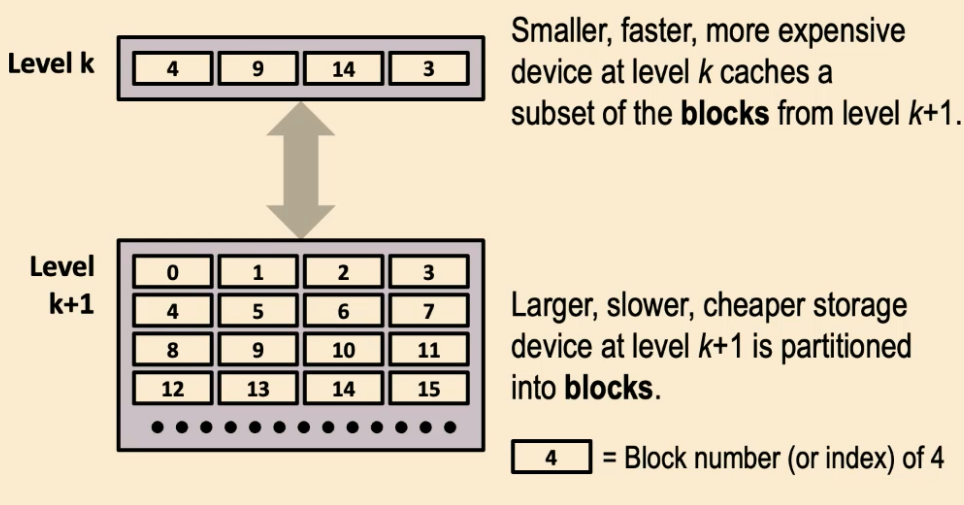
\includegraphics[scale=0.4]{img/cache_retrieve.png}
      \caption{How caches retrieve data from higher levels of memory.} 
      \label{fig:cache_retrieve}
    \end{figure}
  \end{definition}

  \begin{example}[Simple Calculations]
    Given a direct-mapped cache specified by a block size of 8 bytes and a cache capacity of 4 KB, 
    \begin{enumerate}
      \item the cache can hold 512 blocks. 
      \item the block offset field is $\log_2 8 = 3$ bits wide. 
      \item the address \texttt{0x1F = 0b00011111} is in block number $3$ since the last three bits are the offset, and whatever is left (passed through the hashamp, which is simply modulo), is the block number. 
    \end{enumerate}
  \end{example}

  In \textbf{I/O caches}, software keeps copies of cached items in memory, indexed by name via a hash table.

  At the lowest level, registers are explicitly program-controlled, but when accessing any sort of higher memory, the CPU doesn't know whether some data is in the cache, memory, or the disk. That is, 

  \begin{figure}[H]
    \centering 
    \begin{tabular}{|l|l|l|}
      \hline
      \textbf{Level} & \textbf{Storage Type} & \textbf{Management} \\
      \hline
      CPU Registers & Registers & Explicitly program-controlled \\
       & & (e.g., refer to \%rax, \%rbx) \\
      \hline
      L1 Cache & On-chip L1 cache (SRAM) & \multirow{2}{*}{\begin{tabular}[c]{@{}l@{}}Program sees main memory \\ hardware manages caching \end{tabular}} \\
      \cline{1-2}
      L2/L3 Cache & On-chip L2/off-chip L3 & \\
       & cache (SRAM) & \\
      \hline
      Main Memory & Main memory (DRAM) & \multirow{2}{*}{\begin{tabular}[c]{@{}l@{}}Explicitly managed by software \\ (e.g., OS, web browser)\end{tabular}} \\
      \cline{1-2}
      Local Storage & Local secondary storage & \\
       & (local disks) & \\
      \cline{1-2}
      Remote Storage & Remote secondary storage & \\
       & (distributed file systems, web servers) & \\
      \hline
    \end{tabular}
    \caption{} 
    \label{fig:hierarchy2}
  \end{figure}

  Finally, let's compare software vs hardware caches. 

  \begin{definition}[Software Caches]
    When implementing caches in software, there are large time differences (DRAM vs disk, local vs remote), and they can be tailored to specific uses cases. They also have flexible and sophisticated approaches with data structures (like trees) and can perform complex computation. 
  \end{definition}

  Theoretically, when implementing hash tables, you never actually have to evict something. You can have the values of the table to be a linked list where we add to the head. If there is unlimited chaining, we have a full associative cache, and if we have limited chaining (e.g. 5), it is like a 5-way set associative cache. If it goes out of bound, we can implement LRU by removing the tail of the linked list. 

  \begin{definition}[Hardware Caches]
    In hardware caches, there are smaller time differences, needs to be as fast as possible, and parallelization is emphasized. 
  \end{definition}

  There are slightly different implementations of caching, and for each implementation, we will describe 
  \begin{enumerate}
    \item how to load data from memory into the cache, 
    \item how to retrieve data from the cache, 
    \item how to write data to the cache. 
  \end{enumerate}

\subsection{Direct Mapped Cache} 

  A direct mapped cache is a caching implementation when we assume that $E = 1$, which means that for any given memory address, there is only one possible cache line that can store this data at that memory address. That is, the cache is really just a bunch of sets with one cache line each, and each cache line is completely isolated from the others. Whether we load data from memory into cache or try to retrieve data from the cache, it's really the same process. 

  \begin{theorem}[Placement]
    To load data from memory into the cache, which happens when there is a \textbf{cache miss}, we do the following. 
    \begin{enumerate}
      \item The CPU requests a memory address $M = (T, I, O)$. 
      \item There exists a hashmap $H$ that maps the index $I$ to a cache line. 
      \item At line $H(I)$, we can get a cache miss and must load from memory into this cache. 
      \item We wait until the memory has retrieved the data from the portion of the memory. i.e. we wait for the $2^o$ bytes located at addresses $(T, I, 0\ldots 0)$ to $(T, I, 1\ldots 1)$. Call this data $D$. 
      \item The $2^o$ byte string $D$ is stored in the cache data block at line $M(I)$,ready to be used. 
    \end{enumerate}
  \end{theorem}

  \begin{theorem}[Lookup]
    To see whether a requested memory address is in the cache, we do the following. 
    \begin{enumerate}
      \item The CPU requests a memory address $M = (T, I, O)$. 
      \item There exists a hashmap $H$ that maps the index $I$ to a cache line. 
      \item At line $H(I)$, check the cache line's valid bit. If it is not valid, then this is a cache miss and we must go to the memory to retrieve the data, leading to the above process. 
      \item Since there could be multiple $I$ that maps to the same cache line, there will be overlap. But this is where the tag portion comes in. At cache line $H(I)$, the CPU checks the cache tag to see if it matches the memory tag $T$. 
      \item If it does, then we have just found a way to identify the first $t + i$ bits of the requested memory address, and we have gotten a cache hit. Now, we know that the cache's data block holds the data that the program is looking for. We use the low-order offset bits of the address to extract the program's desired data from the stored block. 
    \end{enumerate}
    \begin{figure}[H]
      \centering 
      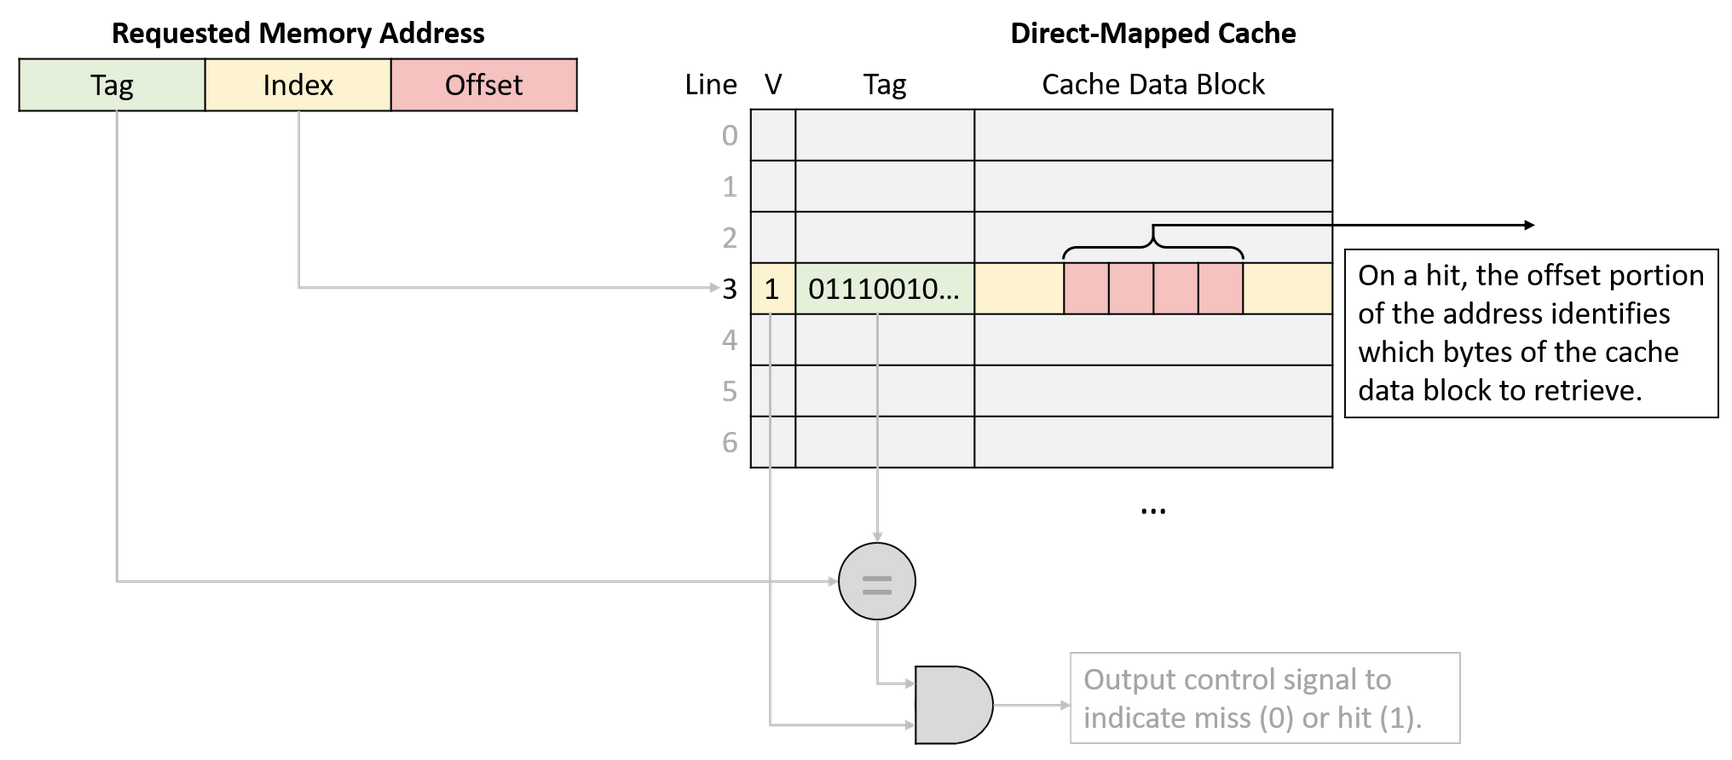
\includegraphics[scale=0.4]{img/cache_request.png}
      \caption{Diagram of a cache request. Note that since the entire data in the memory block stored in the cache, we can take advantage of spatial locality.}  
      \label{fig:cache_request}
    \end{figure}
  \end{theorem}

  So far, we've talked about reading operations, but what about writing to the cache? It is generally implemented in two ways. 

  \begin{definition}[Write-Through, Write-Back Cache]
    Note that when we write data to cache, it does not need to be immediately written to memory, but rather it can be flushed to memory at a later time. This is efficient since if we have repeated operations on a single memory address, we don't have to go back and forth between the CPU and memory. 
    \begin{enumerate}
      \item In a \textbf{write-through cache}, a memory write operation modifies the value in the cache and simultaneously writes the value to the corresponding location in memory. It is always synchronized. 
      \item In a \textbf{write-back cache}, a memory write operation modifies the value stored in the cache's data block, but does \textit{not} update main memory. Instead, the cache sets a \textbf{dirty bit} in the metadata to indicate that the cache block has been modified. The modified block is only written back to memory when the block is replaced in the cache. 

      \begin{figure}[H]
        \centering 
        \begin{tikzpicture}
          % Headers
          \node[anchor=east] at (-0.2, 0.5) {Line};
          \node[anchor=center] at (0.25, 0.5) {V};
          \node[anchor=center] at (0.75, 0.5) {D};
          \node[anchor=center] at (1.5, 0.5) {Tag};
          \node[anchor=center] at (4, 0.5) {Cache Data Block};

          % Table structure
          \foreach \i in {0,1,2,3} {
              \pgfmathsetmacro{\y}{-\i * 0.6}
              
              % Line numbers
              \node[anchor=east, black] at (-0.2, \y) {\i};
              
              % V column
              \draw[thick] (0, \y + 0.3) rectangle (0.5, \y - 0.3);
              
              % D column
              \draw[thick] (0.5, \y + 0.3) rectangle (1.0, \y - 0.3);
              
              % Tag column  
              \draw[thick] (1.0, \y + 0.3) rectangle (2.0, \y - 0.3);
              
              % Data block column
              \draw[thick] (2.0, \y + 0.3) rectangle (6.0, \y - 0.3);
          }
        \end{tikzpicture}
        \caption{A dirty bit (labeled with $D$) is a one bit flag that indicates whether the data stored in a cache line has been modified. When set, the data in the cache line is out o sync with main memory and must be written back (flushed) back to memory before eviction. } 
        \label{fig:dirty_bit}
      \end{figure}
    \end{enumerate}
    As usual, the difference between the designs reveals a trade-off. Write-through caches are less complex than write-back caches, and they avoid storing extra metadata in the form of a dirty bit for each line. On the other hand, write-back caches reduce the cost of repeated writes to the same location in memory.
  \end{definition}

  \begin{theorem}[Replacement]
    Replacement occurs exactly the same way as if we just did a placement and is trivial. We retrieve the data block from the memory and store it in the cache. Direct-mapping conveniently determines which cache line to evict when loading new data. Given new memory $M = (T, I, O)$, you \textit{must} evict the cache line at $H(I)$. 
  \end{theorem}

\subsection{N way Set-Associative Cache}

  Note that for both examples, given a fixed hashmap $H$ it is not possible to store data in two memory addresses $M_1$ and $M_2$ where both $H(I_1) = H(I_2)$. Therefore, the choice of hashing must be done so that it minimizes the number of collisions. So far, we have only considered memory read operations for which a CPU performs lookups on the cache. Caches must also allows programs to store values. However, there is a better way to do this: just construct it so that each set has more than one cache line, and so data in index portions of different memory addresses can be stored in different cache lines.

  In here, we deal with $E \neq 1$, and so there are multiple set each with multiple lines. This means that the cache is more like a 2D array, and when we want to retrieve an index, we must look through the $H(I)$th line in \textit{each} set to see if the tag matches. 

  \begin{theorem}[Lookup]
    To see whether a requested memory address is in the cache, we do the following. 
    \begin{enumerate}
      \item The CPU requests a memory address $M = (T, I, O)$. 
      \item We iterate through each of the $S$ sets in the cache, looking at cache line $M(I)$. 
      \item For each line, we check if it is valid and if so, whether the line tag matches the memory tag. If we get a hit, then we have found the data in the cache. 
    \end{enumerate}

    \begin{figure}[H]
      \centering 
      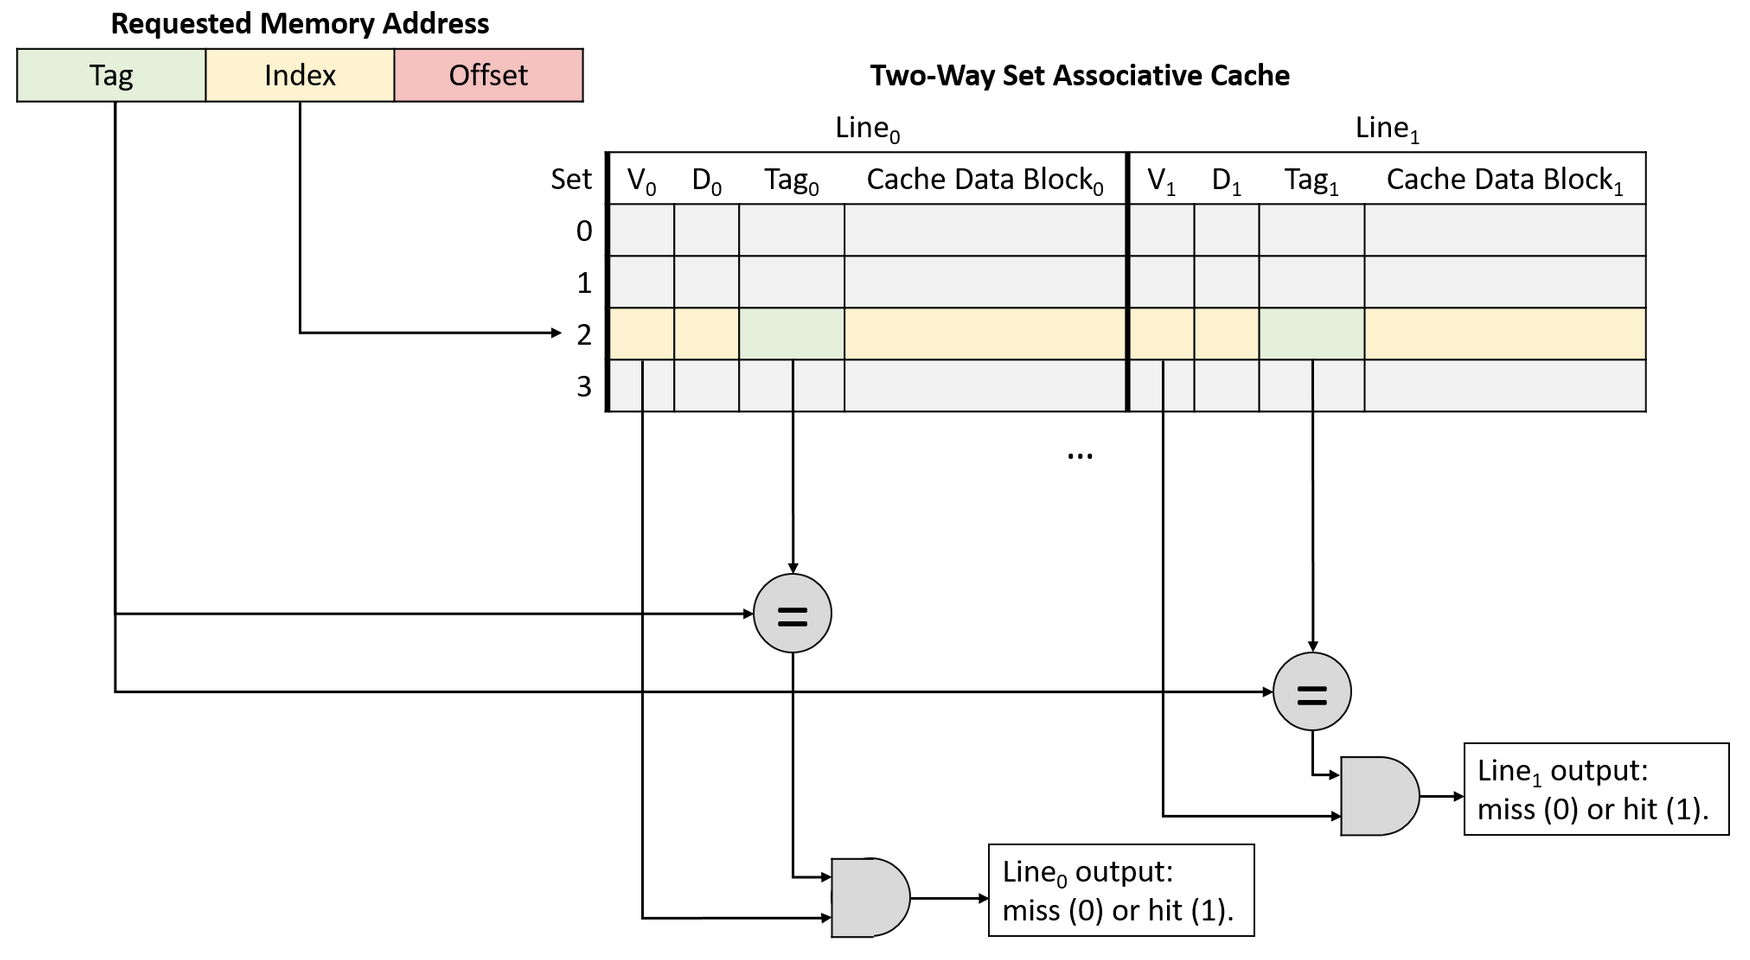
\includegraphics[scale=0.4]{img/retrieve_set_associative.png}
      \caption{Diagram of a 2 set-associative cache.} 
      \label{fig:retrieve_set_associative}
    \end{figure}
  \end{theorem}

  If you have a \textbf{fully associative cache}, then you have one set with $E = C/B$ lines. Therefore, you can really put any memory address data in any cache line. There is a clear tradeoff here. As we increase $N$, we can get more flexibility in using all of our cache space, but the time complexity of retrieving and writing data scales linearly. In fact, this linear scan is too slow for a cache, which is why you need to implement some parallel tag search, but this turns out to be quite expensive to build.\footnote{You have to copy the request tag with a circuit and compare it to all the tags in the cache, which turns out to be a much larger circuit.}

  Though we have a more robust implementation with associative mapping, placement and replacement now face the problem of \textit{which} set to place the data in or evict existing data. 

  \begin{theorem}[Placement]
    To load data from memory into the cache this is trivial since we can just go through the sets, find one where the valid bit is $0$, and just place the data there.  
  \end{theorem}

  In replacement, this is a bit trickier, but using the principle of temporal locality, we can try and replace the least recently used cache. This tries to minimize cache misses, but not slow down the lookup too much. 

  \begin{theorem}[Replacement]
    To replace data on the cache, we use the \textbf{least recently used (LRU)} algorithm. This matches temporal locality, but it also requires some additional state to be kept. 
  \end{theorem}

\subsection{Cache Misses} 

  There are three types of cache misses. 

  \begin{definition}[Cold (Compulsory) Miss]
    A \textbf{cold miss} occurs when the cache is empty and the CPU requests a memory address. This is the first time the CPU is requesting this memory address, and so it must go to the memory to retrieve the data.
  \end{definition}
  
  \begin{definition}[Capacity Miss]
    A \textbf{capacity miss} occurs when the cache is full and the CPU requests a memory address that is not in the cache. This is because the cache is full and so the CPU must evict some data to make space for the new data.
  \end{definition}

  \begin{definition}[Conflict Miss]
    A \textbf{conflict miss} occurs from premature eviction of a warm block. 
  \end{definition}

  Valgrind's cachegrind mode. 



\section{Input Output}

There are 3 file descriptors: STDIN, STDOUT, STDERR

Memory mapped IO. Port mapped IO. 


\section{Disk}

\subsection{Expanding on von Neumann Architecture} 

  So far, our model of the computer has been a simple von Neumann architecture which consists of a CPU and memory. However, there are many other intricacies that are extremely important in practice, and we'll expand on each one by one. 
  
  \begin{definition}[Computer Architecture]
    In our elaborated computer architecture, a computer consists of the components. 
    \begin{enumerate}
      \item A \textbf{CPU} that consists of an arithmetic logic unit (ALU), registers, and a \textbf{bus interface} that controls the input and output. 
      \item The \textbf{IO bridge} that handles communication between everything. 
      \item The \textbf{system bus} that connects the CPU to the IO bridge. 
      \item The \textbf{memory bus} that connects the memory to the IO bridge. 
      \item The \textbf{IO bus} that connects the IO devices and disk to the IO bridge. 
      \item \textbf{IO devices} like mouse, keyboard, and monitor. 
      \item The \textbf{disk controller and disk} that stores data. 
    \end{enumerate} 
    \begin{figure}[H]
      \centering 
      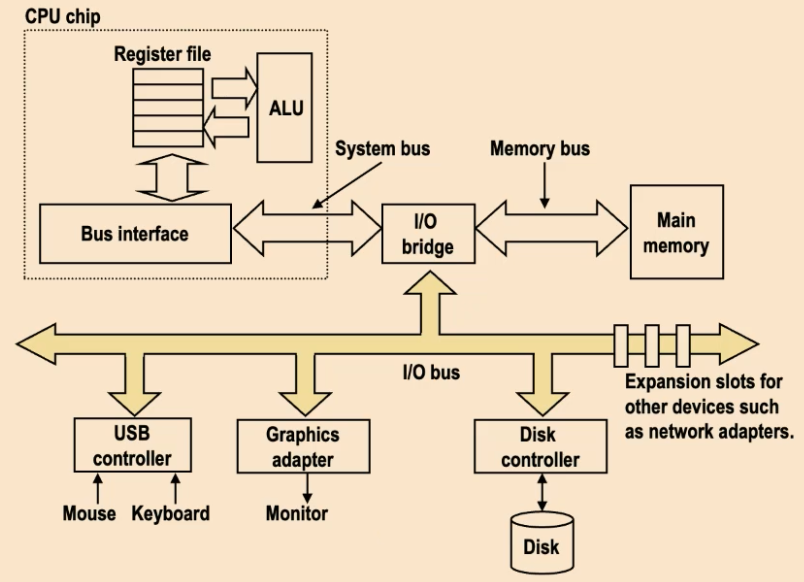
\includegraphics[scale=0.4]{img/io.png}
      \caption{Diagram of the IO bus.} 
      \label{fig:io}
    \end{figure}
  \end{definition}

  We can see from the diagram above that the CPU can directly access registers (since it's in the CPU itself) and the main memory (since it's connected to the memory bus). However, to access something like the disk, it must go through the disk controller. This gives us our first categorization of memory. 

  \begin{definition}[Primary Storage]
    \textbf{Primary storage devices} are directly accessible by the CPU and are used to store data that is currently being processed. This includes CPU registers, cache memory, and RAM. In memory, the basic storage unit is normally a \textbf{cell} (one bit per cell), which is the physical material that holds information. A \textbf{supercell} has address and data widths (number of bits), which is analogous to a lock number and the lock capacity, respectively. It is called random access since it takes approximately the same amount of time to access any cell in memory. There are two primary ways that this is implemented:  
    \begin{enumerate}
      \item \textbf{Static RAM (SRAM)} stores data in small electrical circuits (e.g. latches) and is typically the fastest type of memory. However, it is more expensive to build, consumers more power, and occupies more space, limiting the SRAM storage. 
      \item \textbf{Dynamic RAM (DRAM)} stores data using electrical components (e.g. capacitors) that hold an electrical charge. It is called \textit{dynamic} because a DRAM system must frequently refresh the charge of its capacitors to maintain a stored value. It also requires error correction which introduces redundancy. 
    \end{enumerate}

    \begin{table}[H]
      \centering
      \begin{tabular}{|l|l|l|l|}
      \hline
      \textbf{Device} & \textbf{Capacity} & \textbf{Approx. latency} & \textbf{RAM type} \\ \hline
      Register & 4 - 8 bytes & < 1 ns & SRAM \\ \hline
      CPU cache & 1 - 32 megabytes & 5 ns & SRAM \\ \hline
      Main memory & 4 - 64 gigabytes & 100 ns & DRAM \\ \hline
      \end{tabular}
      \caption{Memory hierarchy characteristics}
      \label{tab:memory_hierarchy}
    \end{table}
  \end{definition}

  \begin{definition}[Secondary Storage]
    \textbf{Secondary storage devices} are not directly accessible by the CPU and are used to store data that is not currently being processed. This includes hard drives, SSDs, and magnetic tapes. There are two primary ways: 
    \begin{enumerate}
      \item \textbf{Spinning disks} store data on a magnetic surface that spins at high speeds.
      \item \textbf{Solid state drives (SSDs)} store data on flash memory chips.
    \end{enumerate}
  \end{definition}

  There are three key components of memory that we should think about: 
  \begin{enumerate}
    \item The \textbf{capacity}, i.e. amount of data, it can store (how large the water tank is). 
    \item The \textbf{latency}, i.e. amount of time it takes for a device to respond with data after it has been instructed to perform a data retrieval operation (how fast the data flows). 
    \item The \textbf{transfer rate} or \textbf{thoroughput}, i.e. amount of data that can be moved between the device and main memory (how wide the pipe is). Naively, with one channel and sequential transfer the transfer rate is one over the latency. 
  \end{enumerate}

  We must provide a good balance of these three qualities, and also note that there are some physical limitations (i.e. latency cannot be faster than speed of light), and this is more effectively done through a hierarchical memory system.

  \begin{figure}[H]
    \centering 
    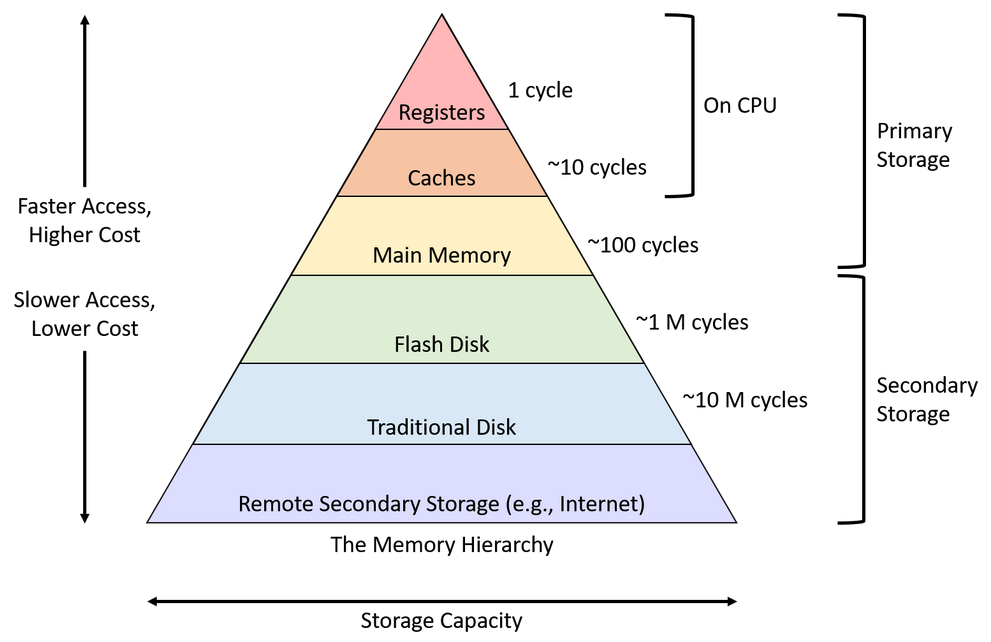
\includegraphics[scale=0.4]{img/memory_hierarchy.png}
    \caption{Memory hierarchy.} 
    \label{fig:memory_hierarchy}
  \end{figure}

  For example when we want to read from the disk, the CPU must request to the bus interface, which travels through the bus interface, I/O bridge, I/O bus, disk controller, and to the disk itself. Then the data goes back through the disk controller, I/O bus, I/O bridge, through the memory bus, and resides in the main memory. Note that disks are block addressed, so it will transfer the entire block of data into the memory. It must specify a \textbf{destination memory address (DMA)}. When the DMA completes, the disk controller notifies the CPU with an \textit{interrupt} (i.e. asserts a special interrupt pin on the CPU), letting it know that the operation has finished. This signal goes through the disk controller to the IO bridge to the CPU. From now on, the CPU knows that there is memory that it can access to run an application loaded in memory. 

\subsection{Disk} 

  \begin{definition}[Hard Disk Drives]
    Back then, there were \textbf{hard disk drives (HDDs)} that literally had a spinning wheel and a needle head that read the data. 
    \begin{figure}[H]
      \centering 
      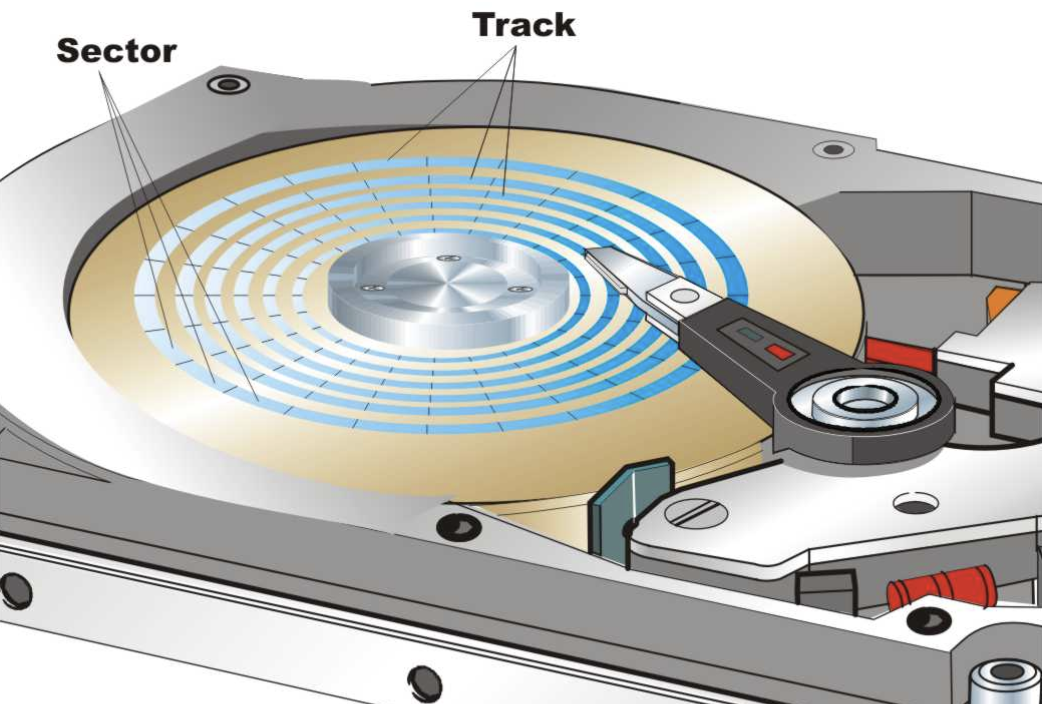
\includegraphics[scale=0.4]{img/hdd.png}
      \caption{Visual diagram of hard disk drive with its sectors. } 
      \label{fig:hdd}
    \end{figure}
    \begin{enumerate}
      \item HDDs are not random access since the data must be sequentially read. This was disadvantageous since the spinning wheel had to spin to the correct location, which took time. The needle also had to move to the correct location, which also took time and therefore read and write speeds were dominated by the time it took to move the needle.
      \item The smallest unit of data that can be read is a complete disk sector (not a single byte like RAM). 
    \end{enumerate}
  \end{definition}

  \begin{definition}[Solid State Drives]
    Now, we have \textbf{solid state drives (SSDs)} that store data on flash memory chips. This is advantageous since there are no moving parts, so the latency is much lower and the latency is not dominated by the time it takes to move the needle. 
    \begin{enumerate}
      \item SSDs are random access. 
      \item The smallest unit of data is a \textbf{page}, which is usually 4KB and maybe for high scale computers 2-4 MB (but on ``Big Data'' applications big but computers, it can be up to 1GB). 
      \item A collection of pages, usually 128 pages, is called a \textbf{block}, making is 512KB. 
    \end{enumerate}
  \end{definition}

  While virtually all RAM and primary storage devices are \textbf{byte addressable} (i.e. you can access any byte in memory), secondary storage devices are \textbf{block addressable} (i.e. you can only access a block of memory at a time). Therefore, to access a single byte in secondary storage, you must first load the entire block into memory, calculate which byte from that block you want, and then access it. Therefore, you need both the block number $x$ and the offset $o$ to access a byte in secondary storage, which is why it is even slower than accessing RAM. 

  \begin{figure}[H]
    \centering 
    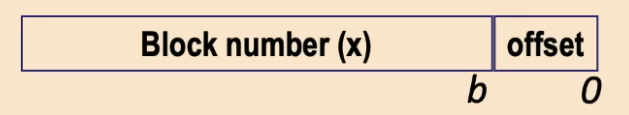
\includegraphics[scale=0.4]{img/block_offset.png}
    \caption{Block offset.} 
    \label{fig:block_offset}
  \end{figure}

  Therefore, you can think of raw data in units of blocks of size $2^b$ for some $b$ bits. 
  \begin{enumerate}
    \item Take the low order $b$ bits of a byte address as an integer, which is the offset of the addressed byte in the block. 
    \item THe rest of the bits are the block number $x$, which is an unsigned long. 
    \item You request the block number $x$, receive the block contents, and then extract the requested byte at offset in $x$ i.e. calculate \texttt{block[x][offset]}. 
  \end{enumerate}



\end{document}
